%%%%%%%%%%%%%%%%%%%%%%%%%%%%%%%%%%%%%%%%%%%%%%%%%%%%%%%%%%%%%%%%%%%%%%%%%%%%%%%
% bt_balazond.tex - Bachelor thesis                                           %
% Subject: bc_emu - portable video game emulator                              %
% Author: Ondrej Balaz <ondra@blami.net>                                      %
%%%%%%%%%%%%%%%%%%%%%%%%%%%%%%%%%%%%%%%%%%%%%%%%%%%%%%%%%%%%%%%%%%%%%%%%%%%%%%%

% Based on K336 template by: Pavel Tvrdik, Daniel Sykora, Michal Valenta

%\documentclass[11pt,twoside,a4paper]{book}
\documentclass[11pt,oneside,a4paper]{book}

% LaTeX packages
\usepackage[czech, english]{babel}
\usepackage[T1]{fontenc}
\usepackage[utf8]{inputenc}
\usepackage{ae,aecompl}
%\usepackage{CJKutf8}
\usepackage{graphicx}
\usepackage{indentfirst}
\usepackage{url}
\usepackage{verbatim}

% local packages
\usepackage{macros_k336}
\usepackage{macros_balazond}

% -----------------------------------------------------------------------------
% Settings
% -----------------------------------------------------------------------------
\newcommand\Department{Katedra počítačů}
\newcommand\Faculty{Fakulta elektrotechnická}
\newcommand\University{České vysoké učení technické v Praze}
\newcommand\labelSupervisor{Vedoucí práce}
\newcommand\labelStudProgram{Studijní program}
\newcommand\labelStudBranch{Obor}

\newcommand\TypeOfWork{Bakalářská práce}
\newcommand\StudProgram{Softwarové technologie a management, Bakalářský}
\newcommand\StudBranch{Softwarové inženýrství}
\newcommand\WorkTitle{Emulátor systému NEC PCEngine}
\newcommand\FirstandFamilyName{Ondřej Baláž}
\newcommand\Supervisor{Ing. Tomáš Davidovič}

% PDF settings
\usepackage[
	pdftitle={\WorkTitle},
	pdfauthor={\FirstandFamilyName},
	bookmarks=true,
	colorlinks=true,
	breaklinks=true,
	urlcolor=red,
	citecolor=blue,
	linkcolor=blue,
	unicode=true,
]
{hyperref}

% -----------------------------------------------------------------------------
% Main document / begin
% -----------------------------------------------------------------------------

\begin{document}

\selectlanguage{czech}

%{
%\pagenumbering{roman} \cleardoublepage \thispagestyle{empty}
%\chapter*{PLACEHOLDER}
%\begin{itemize}
%\item Zadání podepsané děkanem a vedoucím katedry.
%\end{itemize}
%\newpage
%}

% Cover page
\coverpage

% Acknowledgements
\acknowledgements
\noindent
Na tomto místě bych chtěl poděkovat svým přátelům za jejich podporu, trpělivost
a dávky sebevědomí, kterými jsem byl zahrnut v období kdy jsem tuto práci psal.
Slova díku též patří mému zaměstnavateli, který vycházel vstříc mým časovým
potřebám týkajícím se této práce. \\

% Declaration
\declaration{V~Praze dne \today}

% Abstract
\abstract
This thesis describes emulation of video gaming system NEC PCEngine and
implementation of basic functionality of the emulator, with focus on modularity
and portability of source code. In first chapter we present system
specification compiled from various sources, then existing emulators of this
system are reviewed. Then we introduce basic ideas and algorithms used in our
implementation. In last chapter we summarize our results and discuss options
for further improvements, like adding support for other video gaming system
emulators or user interfaces.

\vglue 60mm
\noindent{\Huge \textbf{Abstrakt}}
\vskip 2.75\baselineskip
Bakalářská práce se zabývá problematikou emulace videoherního systému NEC
PCEngine a implementací základní funkčnosti emulátoru s ohledem na modularitu a
přenositelnost kódu. Čtenář je v úvodní části seznámen se zpracovanou
specifikací systému, dále jsou představena existující řešení v oblasti emulace
tohoto systému a rozebrány postupy využívané při implementaci emulátorů.
Následně jsou nastíněny základní myšlenky a postupy využíté při implementaci
modulárního přenositelného emulátoru. Závěrečná část pak pojednává o dosažených
výsledcích a věnuje se možnostem rozšíření navrženého programu o další funkce,
emulátory dalších videoherních systémů a uživatelská rozhraní.

% Table of contents
\setcounter{tocdepth}{2}
\tableofcontents

% List of figures

\listoffigures

% List of tables

\listoftables

% Typographic conventions

%%%%%%%%%%%%%%%%%%%%%%%%%%%%%%%%%%%%%%%%%%%%%%%%%%%%%%%%%%%%%%%%%%%%%%%%%%%%%%%
% bc.tex - Bachelor thesis                                                    %
% Subject: bc_emu - portable video game emulator                              %
% Chapter: Typograficke konvence                                              %
% Author: Ondrej Balaz <ondra@blami.net>                                      %
%%%%%%%%%%%%%%%%%%%%%%%%%%%%%%%%%%%%%%%%%%%%%%%%%%%%%%%%%%%%%%%%%%%%%%%%%%%%%%%

\cleardoublepage
\noindent
\chapter*{Typografické konvence}

V následujícím textu se vyskytuje řada významných klíčových slov. Pro vyšší
přehlednost jsou použity následující typografické konvence:

\begin{itemize}
\item identifikátory a názvy funkcí budou sázeny {\it kurzívou}

\item adresy, offsety a datové konstanty budou uvedeny v hexadecimální soustavě
	sázeny {\tt strojopisem} s použitím prefixu {\tt \$} (v souladu s
	assemblerem pro procesory WDC 65c02 a HuC6280)

\item názvy registrů budou sázeny {\sf groteskem}

\item jména instrukcí budou sázena {\sc kapitálkami}

\item názvy souborů budou sázeny {\tt strojopisem}, v případě uvedení cesty,
	v UNIXové notaci vzhledem ke kořenovému adresáři projektu
\end{itemize}


% -----------------------------------------------------------------------------
% Main document / main
% -----------------------------------------------------------------------------

\mainbodystarts
\normalfont
\parskip=0.2\baselineskip plus 0.2\baselineskip minus 0.1\baselineskip

%%%%%%%%%%%%%%%%%%%%%%%%%%%%%%%%%%%%%%%%%%%%%%%%%%%%%%%%%%%%%%%%%%%%%%%%%%%%%%%
% bc.tex - Bachelor thesis                                                    %
% Subject: bc_emu - portable video game emulator                              %
% Chapter: Uvod                                                               %
% Author: Ondrej Balaz <ondra@blami.net>                                      %
%%%%%%%%%%%%%%%%%%%%%%%%%%%%%%%%%%%%%%%%%%%%%%%%%%%%%%%%%%%%%%%%%%%%%%%%%%%%%%%

\chapter{Úvod}\label{chap:intro}

Neuvěřitelné tempo, kterým se v dnešní době vyvíjejí nové technologie v oblasti
výpočetní techniky, nechává mnohem rychleji, než v jiných oblastech, zestárnout
ty včerejší. Čekání s vývojem software na finální verzi hardware dnes téměř
implikuje vývoj pro zastaralý hardware a v některých odvětvích, jako je třeba
videoherní průmysl, může mít pro autora kritické následky. Emulace je postup,
který pomáhá vývojářům software udržet krok s vývojáři hardware a umožňuje jim
snadno vytvářet software pro hardware, který ještě ve finální podobě
neexistuje. Kromě toho, že je díky emulaci paralelní vývoj software a hardware
běžnou praxí, už i někteří výrobci zpřístupňují ve svých nejmodernějších
výrobcích emulaci těch starších, které si jejich zákazníci
oblíbili.
%\footnote{Největší současní výrobci videoherních konzolí, firmy Sony a
%Nintendo, poskytují službu, v rámci které je možné pomocí emulátorů
%nainstalovaných v konzolích Sony Playstation 3 a Portable, nebo Nintendo Wii
%přehrávat i několik desítek let staré herní tituly.}.

Emulace ale není jen nástroj, který nám pomáhá dostat se s vývojem rychle
kupředu. Můžeme se díky ní ohlédnout i do minulosti, což je jistě zajímavé
právě v oblasti zmíněného herního průmyslu. Za posledních 40 let vznikl
nespočet herních titulů pro 7 generací videoherních konzolí, které si díky
nízkým pořizovacím nákladům a jednoduchosti používání našly své neohrozitelné
místo na trhu. Většina z těchto titulů dávno upadla do zapomění nahrazena
novějšími a emulace videoherních konzolí je tak, vzhledem k nedostupnosti
potřebného hardware, jedinný způsob jak si tyto tituly připomenout.

Jednou z herních konzolí, pro kterou některé z těchto titulů vznikly je NEC
PCEngine. Jedná se o poměrně revoluční koznoli 3. generace, která použitím
16-ti bitové technologie pro obrazový výstup a velice kvalitním zvukovým
výstupem předčila technické možnosti své konkurence. Snad vlivem špatného
marketingu společnosti NEC se nikdy nestala tak populární jako ostatní konzole
této generace, což je společně s tím, že společnost NEC šla cestou použití
komponent navržených výhradně pro tento systém (např. procesoru)
důvodem, proč existuje pouze omezené množství emulátorů této konzole. Právě
zajímavá architektura tohoto systému a poměrně malý počet dostupných emulátorů
jsou hlavním důvodem, proč se tento systém stal předmětem této práce.

Cílem této práce je prostudování architektury videoherního systému NEC
PCEngine, její shrnutí do ucelené technické specifikace (pravděpodobně jedinné
v českém jazyce) a následná analýza, návrh a implementace emulátoru tohoto
systému na jejím základě. Výsledný emulátor by měl, na rozdíl od většiny
existujících implementací, umožňovat snadné rozšíření o podporu dalších
videoherních systémů a být jednoduše přenositelný i na jiné platformy, než
jsou operační systémy osobních počítačů.

\begin{comment}

Vznik a existence videoherního průmyslu jsou přirozenou reakcí výrobců
elektronických zařízení na lidskou potřebu bavit se. Historie videoher sahá až
do roku 1947, kdy bylo patentováno první \uv{zařízení} tohoto druhu - analogový
obvod implementující jednoduchou hru promítanou na stíntko osciloskopu. K
prvním komerčním úspěchům v této oblasti však vedla ještě dlouhá cesta, než v
roce 1972 společnost Atari začala vyrábět legendární videohru {\em PONG}, která
svým jednoduchým principem, provedením umožňujícím provoz na běžném televizoru
a nízkou cenou zpřístupnila tento nový druh zábavy široké veřejnosti.

Popularita a úspěch videohry {\em PONG} byly důležitým impulzem pro vznik
konceptu videoherní konzole, elektronického zařízení pro domácí zábavu. Díky
jednoduchosti obsluhy, nízkým pořizovacím nákladům a rozmanité škále žánrů
herních programů si v průběhu uplynulých 40-ti let vybudovalo 7
generací\footnote{Dělení videoherních konzolí na generace se odvíjí od velkých
technických kroků v této oblasti, jako je přechod od 8-mi bitů k 16-ti atd.,
více viz.~\cite{wwwWikiConsole}} videoherních konzolí neotřesitelné místo na
trhu.

V průběhu těchto 40-ti let také vzniklo nesčetné množství více či méně
populárních herních programů, které s příchodem nových technologií, a tedy i
videoherních konzolí nových generací, zastárly. Původní hardware nutný ke
spuštění těchto programů je v dnešní době prakticky nesehnatelný a jedinnou
možností jak se k těmto programům vrátit je emulace videoherní konzole, pro
kterou byly určeny.

Cílem této práce je nastudovat architekturu videoherní konzole NEC PCEngine a
na základě 

Vrcholu své popularity dosáhly videoherní konzole v letech 1983-1995, tedy v
době, kdy už byla běžně dostupná osobní výpočetní technika, ale v případě, že
by měla sloužit pouze jako zdroj zábavy, byla její cena stále příliš vysoká.
Dostupné technologie společně s důmyslným návrhem však umožnily přinést na
trh levné, ale přesto výkonné videoherní konzole 3. generace, které se
vyznačovaly detailní a propracovanou grafikou ve vysokém rozlišení, kvalitním
zvukovým výstupem a novými způsoby ovládání.

Příchod videoherních konzolí 3. generace měl za následek nové možnosti při
vývoji herních programů, díky čemuž právě v této době vznikla řada
nezapomenutelných titulů (např. {\em Final Fantasy}, {\em Super Mario Bros.},
{\em The Legend of Zelda}, {\em Castlevania}, {\em Contra}), které možná byly
nebo budou překonány po stránce technického zpracování, ale nikoliv po stránce
originality a nápadu, o čemž svědčí i fakt, že velké množství dnešních
videoherních titulů z nich čerpá, nebo je jejich kopií oblečenou do \uv{nového
kabátu}.

Právě do 3. generace videoherních konzolí patří systém NEC PCEngine. Jeho
unikátní architektura založená na 8-mi bitovém hlavním procesoru a 16-ti
bitovém grafickém subsystému


\end{comment}

%%%%%%%%%%%%%%%%%%%%%%%%%%%%%%%%%%%%%%%%%%%%%%%%%%%%%%%%%%%%%%%%%%%%%%%%%%%%%%%
% bc.tex - Bachelor thesis                                                    %
% Subject: bc_emu - portable video game emulator                              %
% Chapter: Specifikace                                                        %
% Author: Ondrej Balaz <ondra@blami.net>                                      %
%%%%%%%%%%%%%%%%%%%%%%%%%%%%%%%%%%%%%%%%%%%%%%%%%%%%%%%%%%%%%%%%%%%%%%%%%%%%%%%

\chapter{NEC PCEngine}\label{chap:spec}

Znalost principů fungování emulovaného systému a systému samotného je jedním z
klíčových předpokladů pro úspěšnou implementaci emulátoru. U videoherních
systémů je získání technické specifikace většinou obtížné, protože se jedná o
uzavřené produkty a jejich výrobci mají komerční a jiné důvody, proč oficiální
dokumentaci nezveřejňovat a to dokonce i v době, kdy pro ně konkrétní systém už
nemá žádný komerční význam.

Autoři emulátorů jsou tak odkázání na metody reverzního
inženýrství\footnote{Snaha o odkrytí principu na kterém funguje zařízení, např.
za účelem jeho chování napodobit.}, přičemž vzniká často používaná neoficiální
dokumentace, která, i přes svůj přínos, může být neúplná nebo nepřesná. V
případě systému NEC PCEngine tento proces navíc komplikuje malá popularita a
tedy i malý počet zainteresovaných vývojářů a fakt, že jeho výrobce šel cestou
použití zcela specifického hardware (ostatní systémy téže generace byly téměř
bez výhrady postaveny na dobře zdokumentovaných procesorech MOS 6502 či Zilog
Z80).

Sekce~\ref{chap:spec_history}, která otevírá tuto kapitolu, stručně představuje
videoherní systém NEC PCEngine a stručně pojednává o jeho historii.

Protože pravděpodobně neexistuje žádný dokument, který by shrnoval dostupné
technické specifikace základní verze systému NEC PCEngine na jednom místě, ale
jen dílčí dokumenty specializující se na technickou specifikaci určité částí
systému NEC PCEngine, je v sekci~\ref{chap:spec_hw} předložena co možná
nejkompletnější\footnote{Z hlediska specifik systému NEC PCEngine, pro
přehlednost není uvedena např. kompletní specifikace procesoru WDC 65c02 z nějž
vychází procesor HuC6280 použitý v systému NEC PCEngine, ale jen odlišnosti
použitého procesoru HuC6280.} specifikace tohoto systému, která je založena
nejen na zmiňovaných dokumentech~\cite{Ormston06, MacDonald02, Schleussinger98,
Clifford, Woodford94, LaMothe05, www65c02}, ale také na studiu zdrojových kódů
existujících emulátorů \cite{wwwMednafen, wwwOotake} a konečně i vlastních
zkušenostech nabytých při implementaci emulátoru.

Poslední sekce~\ref{chap:spec_sw} této kapitoly pak stručně pojednává o
software dostupném pro systém NEC PCEngine.

% -----------------------------------------------------------------------------
% Historie
% -----------------------------------------------------------------------------

\section{Historie}\label{chap:spec_history}

NEC PCEngine je hybridní videoherní konzole vyvinutá japonskými společnostmi
HudsonSoft a NEC v roce 1987. Hybridní je nazývána proto, že ačkoliv hlavní
procesor je 8-mi~bitový, jako u většiny herních konzolí 3. generace
(Nintendo Famicom, Sega Master System, Atari 7800), grafický systém je plně
16-ti bitový. Vzhledem k tomu, že NEC PCEngine bylo uvedeno do prodeje v roce
1987, NEC předběhl své hlavní rivaly v použití 16-ti bitové technologie a z ní
vyplývajících výhod o celou jednu generaci herních konzolí. Pokročilý 6-ti
kanálový zvukový subsystém dovoloval kromě přehrávání samplů i jednoduchou
zvukovou syntézu a modulaci zvuku. Je jen s podivem, že tak pokročilý systém,
jakým bezesporu ve své době NEC PCEngine byl, zdaleka nedosáhl světové obliby
na alespoň stejné úrovni jako ostatní videoherní konzole téže
generace.~\cite{wwwClassicGaming, wwwWikiTurboGrafx}

\begin{figure}[ht]
\begin{center}
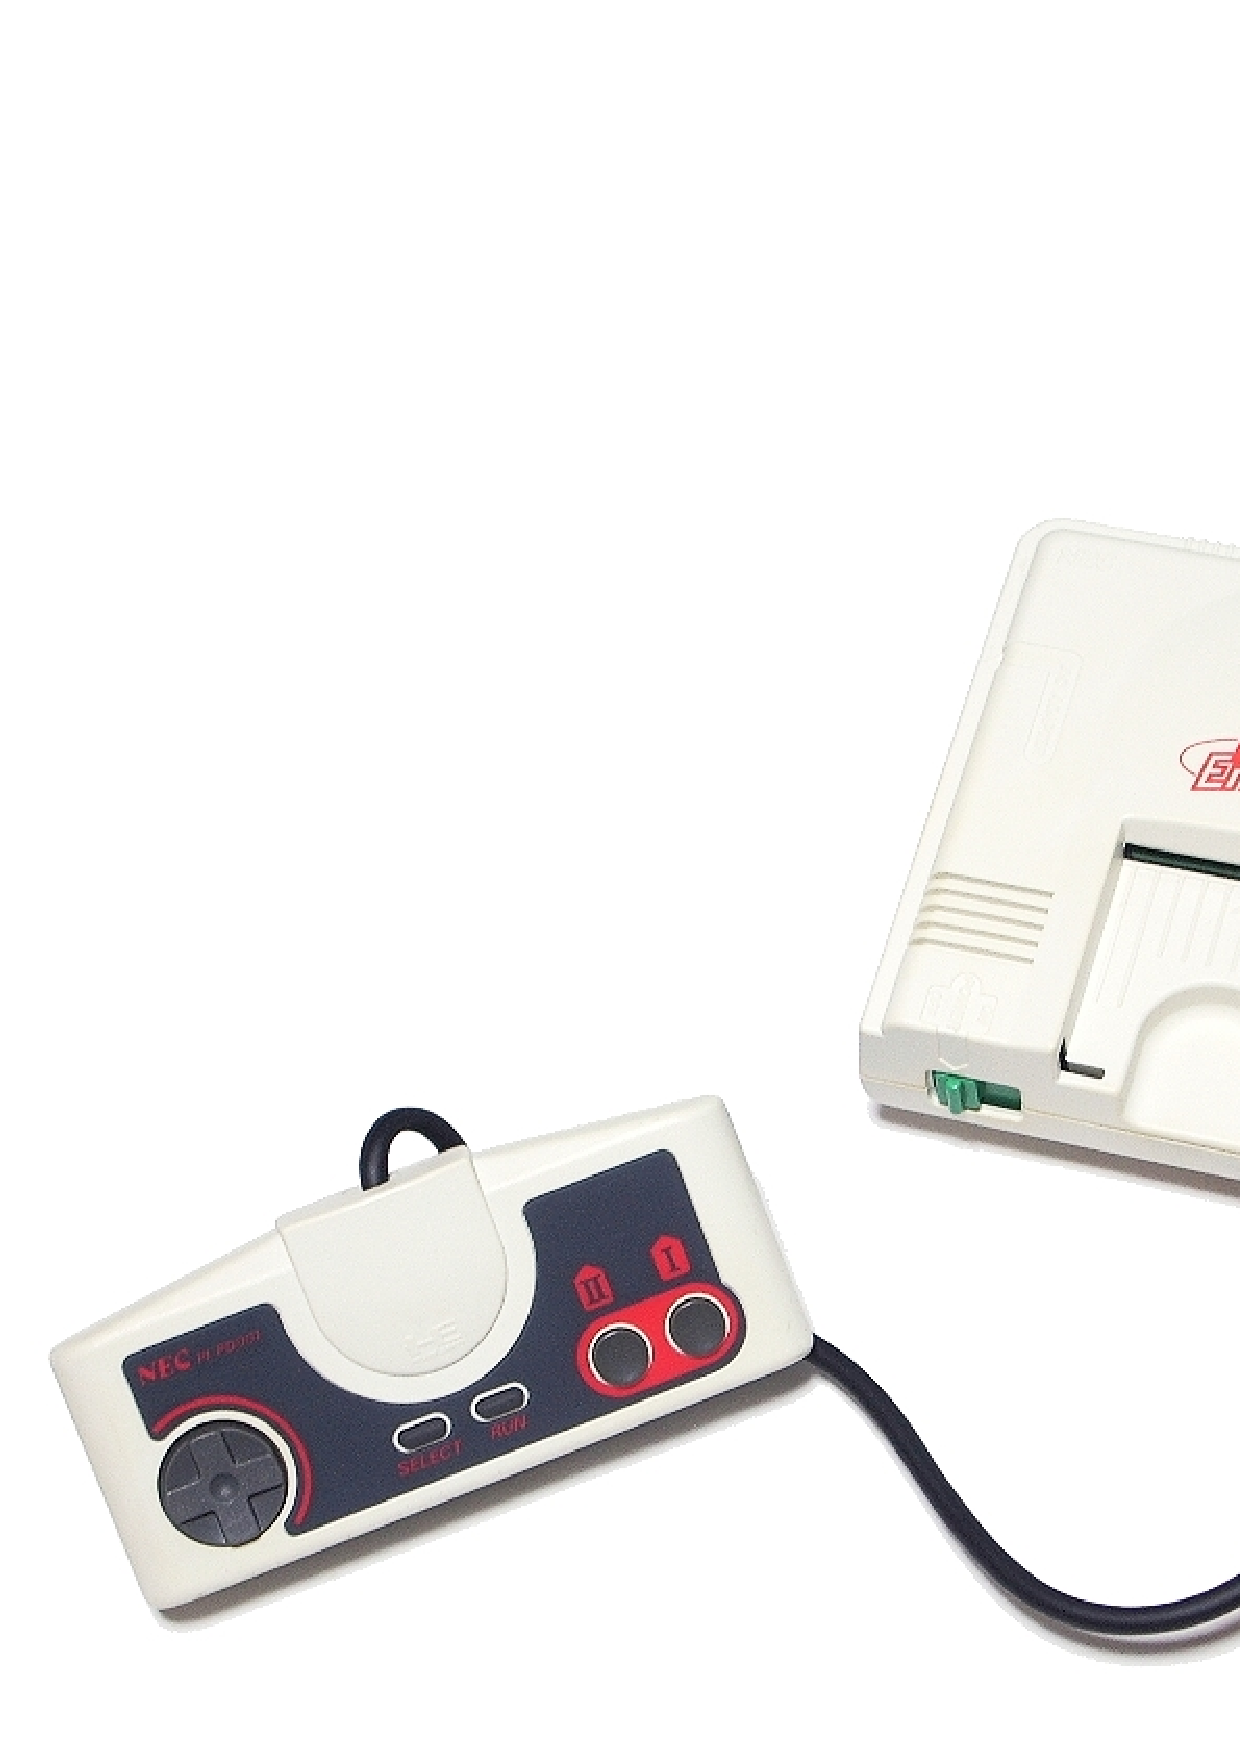
\includegraphics[width=6cm]{fig/pce_photo}
\caption{Systém NEC PCEngine, základní varianta\label{fig:pce_photo}}
\end{center}
\end{figure}

Systém NEC PCEngine byl firmou NEC postupně inovován. Kromě rozšíření paměti a
přidání vstupního portu pro další herní ovladač(e) se v následujících verzích
dočkala i rozšíření (jako první videoherní konzole na světě) o CD-ROM jednotku
a další grafický koprocesor. Mírně modifikovaný systém byl od roku 1989 v malém
nákladu exportován z Japonska do Severní Ameriky a Evropy pod názvem NEC
TurboGrafx 16, kde se ale vůbec neprosadil vlivem špatného marketingu a
nedostatku vývojářů her. {\em Pozn.: popsaná rozšíření ani modifikace nejsou v
práci uvažovány.}~\cite{wwwClassicGaming, BartonLoguidice09}

S příchodem plně 16-ti bitových herních konzolí 4. generace (Sega Genesis,
Super Nintendo Entertainment System) v roce 1991 přišel systém NEC PCEngine o
své místo na trhu a po neúspěších s dalším systémem (PC FX32) opouští NEC
videoherní průmysl.~\cite{wwwWikiTurboGrafx}

Zajímavostí pro doplnění je, že svými fyzickými rozměry 14cm x 14cm x 3.8cm se
NEC PCEngine zapsalo do Guinnessovy knihy rekordů jako nejmenší nepřenosná
videoherní konzole.~\cite{Guinness08}

% -----------------------------------------------------------------------------
% Hardware NEC PCEngine
% -----------------------------------------------------------------------------

\section{Hardware}\label{chap:spec_hw}

Základní verze NEC PCEngine je vybavena 8~KB operační paměti (RAM) a 64~KB
videopaměti (VRAM). Hlavní procesor HuC6280 řídí zpracování programu uloženého
v paměti určené pouze pro čtení (ROM) na výměnné čipové kartě
HuCard\footnote{Čipové karty HuCard měly formát kreditní karty, čímž se zásadně
lišily od podstatně větších zásuvných modulů rivalských systémů od společností
Nintendo a Sega.}. Dále zajišťuje ozvučení programu pomocí programovatelného
generátoru zvuků (Programmable Sound Generator, PSG) o 6ti kanálech a
zpracování vstupu z portu herního ovladače.

O obrazový výstup se stará dvojice 16-ti bitových grafických pomocných
procesorů, konkrétně kontrolér pro zobrazování (Video Display Controller, VDC)
HuC6270 a enkodér barev (Video Color Encoder, VCE) HuC6260. Ty společně
zajišťují zobrazení v rozlišeních až 512x240 pixelů v 9-ti bitové barevné
hloubce (512 barev celkem, na obrazovce zobrazitelných maximálně 482 barev)
pomocí RF (anténního) výstupu na televizní set ve standardu NTSC.~\cite{wwwWikiTurboGrafx}

%
% CPU
%

\subsection{CPU}\label{chap:spec_hw_cpu}

Hlavní procesor celého systému (Central Processing Unit, CPU) nese označení
HuC6280 a vychází z mikroprocesoru WDC 65c02 společnosti Western Digital, jehož
specifikaci~\cite{www65c02} rozšiřuje o řadu instrukcí a adresních módů a
přidává některá, pro účely videoherního systému, specifická periferní zařízení.
Jedná se o 8-mi bitový procesor schopný operovat na frekvencích 3.58~MHz a
7.16~MHz (lze libovolně měnit za běhu programu vykonáním dvou speciálních
instrukcí {\sc csl} a {\sc csh}). Architektura systému je znázorněna na
obr.~\ref{fig:pce_arch}.

\begin{figure}[ht]
\begin{center}
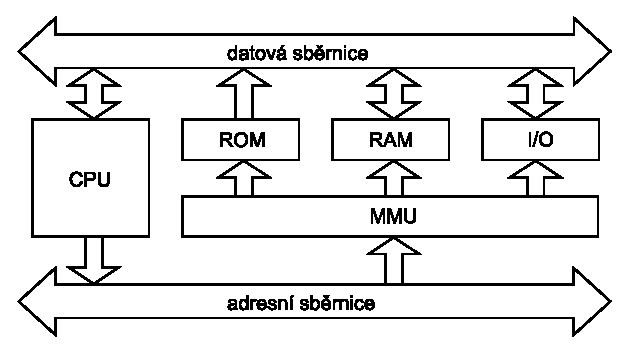
\includegraphics[width=10cm,height=5.3cm]{fig/pce_arch}
\caption{Architektura systému NEC PCEngine\label{fig:pce_arch}}
\end{center}
\end{figure}

Z hlediska endianity je CPU HuC6280 \uv{little-endian}\footnote{Při práci s
vícebajtovými položkami je nejméně významný bajt je v paměti uložen na nejnižší
adrese.}. Tento fakt se pochopitelně týká i obou grafických pomocných procesorů
VDC HuC6270 a VCE HuC6260. V následujícím textu se s touto skutečností mlčky
počítá.

Jak již bylo zmíněno, oproti WDC 65c02 disponuje CPU HuC6280 řadou periferních
zařízení: jednotkou obsluhy přerušení, 8-mi bitovým paralelním I/O portem (pro
herní ovladač), jednotkou správy paměti (mapovačem), časovačem a
programovatelným generátorem zvuku (PSG).

% Registry

\subsubsection{Registry}\label{chap:spec_hw_cpu_reg}

\begin{description}
\item[{\sf A}] Střadač (Accumulator) \\
	Bezpochyby nejdůležitější registr CPU HuC6280. Slouží jako zdrojový, cílový
	nebo oba operandy pro většinu instrukcí. Je to jedinný registr, který lze
	použít s řadou insturkcí pro provádění matematických výpočtů. Délka
	registru {\sf A} je 8 bitů.

\item[{\sf X}] Indexový registr X (Index X) \\
	Jedná se o registr obecného použití často využívaný při některých adresních
	módech s nepřímou adresou. Je též používán jako vnitřní čítač pro cykly.
	Délka registru {\sf X} je 8 bitů.

\item[{\sf Y}] Indexový registr Y (Index Y) \\
	Jedná se opět o registr obecného použítí s podobným využitím a vlastnostmi
	jako má registr {\sf X}. Délka registru {\sf Y} je 8 bitů.

\item[{\sf PC}] Čítač programu (Program counter) \\
	Obsahuje adresu instrukce, která se má vykonat. Ve chvíli kdy dojde k
	vykonání instrukce je hodnota čítače automaticky
	zvýšena/změněna\footnote{Ke změnám, které nemusí být inkrementací dochází
	např. při použití instrukcí skoku nebo volání podprogramu.}. Délka registru
	{\sf PC} je 16 bitů.

\item[{\sf S}] Ukazatel na zásobník (Stack pointer) \\
	Obsahuje adresu prvního volného místa v zásobníku\footnote{Místo v paměti
	určené k dočasným odložení hodnot programem.}. Délka registru {\sf S} je 8
	bitů.

\item[{\sf P}] Příznakový registr (Program flags) \\
	Tento velice významný registr obsahuje bitové pole s příznaky indikujícími
	aktuální stav procesoru po poslední provedené operaci. Některé z těchto
	příznaků mohou být i nastaveny z programu. Jednotlivé příznaky jsou uvedeny
	v tabulce~\ref{tab:cpu_flags}. Význam jednotlivých příznaků následuje.

	\begin{table}[ht]
	\begin{center}
	\begin{tabular}{|c|c|c|c|c|c|c|c|c|}
	\hline
	\textbf{Bit} & 7 & 6 & 5 & 4 & 3 & 2 & 1 & 0 \\
	\hline
	\textbf{Příznak} & N & O & T & B & D & I & Z & C \\
	\hline
	\end{tabular}
	\end{center}
	\caption{Příznaky indikované registrem P CPU HuC6280\label{tab:cpu_flags}}
	\end{table}

	\begin{description}
	\item[N] Záporný výsledek (Negative) \\
		Stav \uv{1} tohoto příznaku indikuje,
		že poslední operace nastavila nejvyšší bit výsledku.

	\item[O] Přetečení (Overflow) \\
		Stav \uv{1} tohoto příznaku indikuje přetečení (nesprávný přenos
		nejvyššího bitu). Používá se hlavně při aritmetických operacích, kde
		záleží na znaménku.

	\item[T] Set režim (Set mode) \\
		Speciální akumulátorový režim, souvisí s instrukcí {\sc set}. Více o
		tomto režimu lze nalézt např. v~\cite{MacDonald02}.

	\item[B] Přerušení (Break) \\
		Stav \uv{0} tohoto příznaku indikuje hardwarové přerušení. Slouží k
		rozlišení hardwarových přerušení od použití instrukce {\sc
		brk}\footnote{Instrukce {\sc brk} způsobí softwarové přerušení.}.

	\item[D] Decimální mód (Decimal mode) \\
		Stav \uv{1} tohoto příznaku indikuje, že některé matematické instrukce
		počítají v BCD kódu namísto binárního. Tento příznak lze přímo
		nastavit.

	\item[I] Zákaz přerušení (Interrupt disable) \\
		Stav \uv{1} tohoto příznaku indikuje zákaz všech běžných přerušení (s
		vyjímkou Non-maskable interrupt (NMI). Tento příznak lze přímo
		nastavit.

	\item[Z] Nula (Zero) \\
		Nastavení tohoto příznaku indikuje, že výsledek poslední operace byl
		\uv{nula}.

	\item[C] Přenos (Carry) \\
		Stav \uv{1} tohoto příznaku indikuje přenos bitu z poslední vykonané
		operace.
	\end{description}

	Délka registru {\sf P} je 8 bitů.

\item[{\sf MPR0-7}] Registr paměťové stránky (Memory page register) \\
	Každý z 8 {\sf MPR} registrů obsahuje index paměťové stránky, ze kterého se
	počítá výsledná 21-bitová adresa. Délka registru {\sf MPR0-7} je 8x8 bitů.

\item[{\sf CS}] Rychlost hodin (Clock speed) \\
	Skrytý jednobitový registr ovládaný pomocí dvou instrukcí ({\sc csl} a {\sc
	csh}). Pokud je hodnota tohoto registru \uv{1}, frekvence procesoru je
	7.16~MHz. V případě, že je hodnota registru \uv{0}, pak je frekvence
	procesoru poloviční (tedy 3.58~Mhz). Délka registru {\sf CS} je 1 bit.
	\cite{Ormston06}
\end{description}

% Pamet

\subsubsection{Paměť}\label{chap:spec_hw_cpu_memory}

Hlavní změnou oproti WDC 65c02 je způsob práce s pamětí. CPU HuC6280 je schopný
adresovat 64~KB paměti logickou adresou z fyzického paměťového prostoru 2~MB.
Adresa je oproti původním 16-ti bitům dlouhá 21 bitů a pro přístup k paměti se
využívá 8 mapovacích registrů {\sf MPR0-7}, z nichž každý obsahuje index 8~KB
velké stránky z fyzického paměťového prostoru. Specifikace příslušného {\sf
MPR} registru je prováděna pomocí tří horních bitů logické adresy. Práce s
těmito registry probíha pomocí speciálních instrukcí: {\sc tam} a {\sc tma}.
Rozdělení logické paměti do stránek je znázorněno v tabulce~\ref{tab:cpu_mem}.

\begin{table}[hb]
\begin{center}
\begin{tabular}{|c|l|}
\hline
\textbf{Stránka} & \textbf{Logický adresní prostor} \\
\hline
0 & {\tt \$0000} - {\tt \$1FFF}\\
1 & {\tt \$2000} - {\tt \$3FFF}\\
2 & {\tt \$4000} - {\tt \$5FFF}\\
3 & {\tt \$6000} - {\tt \$7FFF}\\
4 & {\tt \$8000} - {\tt \$9FFF}\\
5 & {\tt \$A000} - {\tt \$BFFF}\\
6 & {\tt \$C000} - {\tt \$DFFF}\\
7 & {\tt \$E000} - {\tt \$FFFF}\\
\hline
\end{tabular}
\end{center}
\caption{Rozdělení logické paměti CPU HuC6280 do stránek\label{tab:cpu_mem}}
\end{table}

Pro dokončení představy o způsobu adresace paměti je v
tabulce~\ref{tab:cpu_banks} znázorněno rozdělení fyzického adresního
prostoru (2~MB) na 256 8~KB velkých bank.

\begin{table}[ht]
\begin{center}
\begin{tabular}{|c|l|}
\hline
\textbf{Banky} & \textbf{Význam} \\
\hline
{\tt \$00} - {\tt \$7F} & paměť ROM výměnného modulu HuCard
	(viz.~\ref{chap:spec_hw_rom})\\
{\tt \$80} - {\tt \$F7} & {\em nevyužito}\\
{\tt \$F8} - {\tt \$FB} & RAM (pouze 8~KB 4x zrcadlených)\\
{\tt \$FC} - {\tt \$FE} & {\em nevyužito}\\
{\tt \$FF} & vstupně-výstupní banka (tzv. \uv{I/O page},
	viz.~\ref{chap:spec_hw_cpu_peripheral})\\
\hline
\end{tabular}
\end{center}
\caption{Rozdělení fyzické paměti CPU HuC6280 do bank\label{tab:cpu_banks}}
\end{table}

Výpočet 21-bitové adresy probíhá tak, že pomocí horních 3 bitů 16-ti bitové
logické adresy je zvolen jeden z {\sf MPR} registrů. Z něj je načten 8-mi
bitový index banky, který je posléze posunut o 13 bitů vlevo a sečten se
zbývajícími 13ti bity logické adresy (offsetem ve stránce). Výsledkem je
fyzická 21-bitová adresa~\cite{Ormston06}. Postup výpočtu fyzické
adresy je znázorněn na obr.~\ref{fig:cpu_addr}.

Ve výchozím stavu je pomocí {\sf MPR} registrů banka {\tt \$FF} mapována
jako stránka 0, banka {\tt \$F8} jako stránka 1 a konečně banka {\tt \$00}
jako stránka 7. {\bf Následující text s tímto mapováním počítá při uvádění
logických adres.}

Jen pro kompletnost a lepší orientaci v dalším textu (zejména pak v sekci
\ref{chap:spec_hw_cpu_instr}) uvádíme fakt, že veškeré operace se zásobníkem a
stránkou nula\footnote{První stránka adresního prostoru.} vždy pracují v
rozsahu logických adres {\tt \$2000} - {\tt \$2FFF}, což odpovídá použití
mapovacího registru {\sf MPR1} a fyzickým adresám {\tt \$1F0000} pro počátek
stránky nula a {\tt \$1F0100} pro dno zásobníku.

\begin{figure}[hb]
\begin{center}
\vspace{1.2cm}
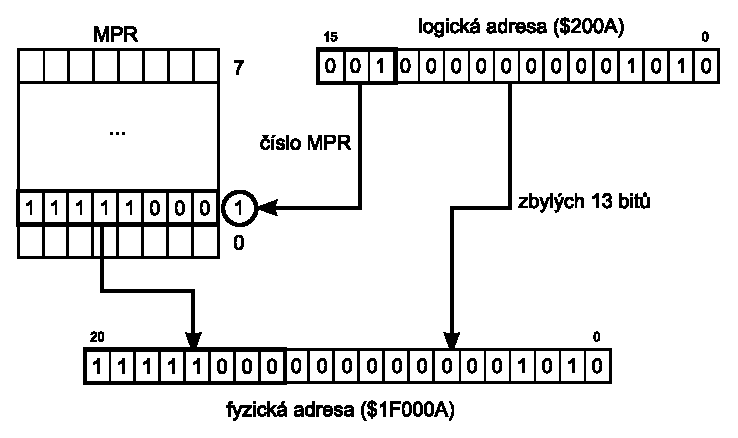
\includegraphics[width=12cm,height=7cm]{fig/pce_banks}
\caption{Výpočet fyzické adresy\label{fig:cpu_addr}}
\end{center}
\end{figure}

\newpage

% Instrukcni sada

\subsubsection{Instrukční sada}\label{chap:spec_hw_cpu_instr}

CPU HuC6280 rozšiřuje instrukční sadu WDC 65c02 (která je podrobně popsána,
včetně možnosti adresace operandů a vlivu na příznakový registr pro každou
instrukci, např. v \cite{www65c02}) o několik specifických instrukcí a způsobů
adresace operandů.

Jedná se o následující výčet instrukcí. Počty cyklů, možnosti adresace operandů
a vliv na příznakový registr pro jednotlivé instrukce lze nalézt v
\cite{Ormston06}.

\begin{description}
\item[{\sc bsr}] (Branch To Subroutine) \\
	Uloží absolutní adresu následující instrukce sníženou o jedna na zásobník a
	skočí do subrutiny.

\item[{\sc cla}] (Clear Accumulator) \\
	Nastaví hodnotu střadače na \uv{0}.

\item[{\sc clx}] (Clear Index X) \\
	Nastaví hodnotu indexového registru {\sf X} na \uv{0}.

\item[{\sc cly}] (Clear Index Y) \\
	Nastaví hodnotu indexového registru {\sf Y} na \uv{0}.

\item[{\sc csh}] (Clock Select High) \\
	Slouží ke změně obsahu skrytého registru {\sf CS} na \uv{1}. Procesor se přepne
	na kmitočet 7.16~MHz.

\item[{\sc csl}] (Clock Select Low) \\
	Slouží ke změně obsahu skrytého registru {\sf CS} na \uv{0}. Procesor se přepne
	na kmitočet 3.58~MHz.

\item[{\sc sax}] (Swap Accumulator And Index X) \\
	Prohodí obsah střadače a indexového registru {\sf X}.

\item[{\sc say}] (Swap Accumulator And Index Y) \\
	Prohodí obsah střadače a indexového registru {\sf Y}.

\item[{\sc set}] (Set Decimal Memory Operation Flag) \\
	Přepne procesor do akumulátorového módu (decimálního) na jeden instrukční
	cyklus (nastaví příznak \uv{T} na \uv{1}).

\item[{\sc sxy}] (Swap Index X And Index Y) \\
	Prohodí obsah indexových registrů {\sf X} a {\sf Y}.

\item[{\sc st0}] (Store At VDC Address 1) \\
	Zapíše data pro VDC HuC6270 do hardwarového registru 0 (fyzická adr. {\tt \$1FE000}).

\item[{\sc st1}] (Store At VDC Address 2) \\
	Zapíše data pro VDC HuC6270 do hardwarového registru 1 (fyzická adr. {\tt \$1FE002}).

\item[{\sc st2}] (Store At VDC Address 3) \\
	Zapíše data pro VDC HuC6270 do hardwarového registru 2 (fyzická adr. {\tt \$1FE003}).

\item[{\sc tai}] (Transfer 'from' Alternate 'to' Increment) \\
	Přenese blok dat z adresy {\it from} na adresu {\it to} tak, že v každém cyklu
	zamění adresu {\it from} s obsahem paměti na této adrese a zvýší adresu
	{\it to} o \uv{1}.

\item[{\sc tam}] (Transfer Accumulator To MPR) \\
	Přenese obsah střadače do mapovacího registru.

\item[{\sc tdd}] (Transfer 'from' Decrement 'to' Decrement) \\
	Přenese blok dat z adresy {\it from} na adresu {\it to} tak, že v každém cyklu
	obě adresy sníží o \uv{1}.

\item[{\sc tia}] (Transfer 'from' Increment 'to' Alternate) \\
	Přenese blok dat z adresy {\it from} na adresu {\it to} tak, že v každém cyklu
	sníží adresu {\it from} o \uv{1} a zamění adresu {\it to} s obsahem paměti
	na této adrese.

\item[{\sc tii}] (Transfer 'from' Increment 'to' Increment) \\
	Přenese blok dat z adresy {\it from} na adresu {\it to} tak, že v každém cyklu
	obě adresy zvýší o \uv{1}.

\item[{\sc tin}] (Transfer 'from' Increment 'to' Does Nothing) \\
	Přenese blok dat z adresy {\it from} na adresu {\it to} tak, že v každém cyklu
	zvýší adresu {\it from} o \uv{1}.

\item[{\sc tma}] (Transfer MPR To Accumulator) \\
	Přenese obsah mapovacího registru do střadače.

\item[{\sc tst}] (Test Bits) \\
	Otestuje bity mezi dvěma operandy kde jeden je přímý a jeden z paměti.
	Nastaví příznakový registr tak, že indikuje stav horních dvou bitů hodnoty
	načtené z paměti pomocí příznaků \uv{N} a \uv{O} a shodu alespoň v jednom
	bitu pomocí příznaku \uv{Z}.
\end{description}

\newpage

% Rezimy adresace operandů

\subsubsection{Režimy adresace operandů}\label{chap:spec_hw_cpu_addr}

Režimy adresace operandů instrukcí CPU HuC6280 jsou uvedeny v
tabulce~\ref{tab:cpu_addrmodes}. Většina instrukcí je použitelná jen s
několika ze všech vyjmenovaných způsobů adresace operandů, které v jejím
případě dávají smysl (např. jedinná instrukce, která může použít nepřímou
adresaci nebo nepřímou adresaci s indexem je {\sc jmp}). Způsoby adresace
operandů specifické pro CPU HuC6280 jsou uvedeny ve spodní části
tabulky~\ref{tab:cpu_addrmodes} oddělené čarou a popsány v následujícím textu.
Podrobnosti o jednotlivých způsobech adresace operandů lze nalézt v
\cite{www65c02, Ormston06}.

\begin{table}[h!]
\begin{center}
\begin{tabular}{|l|l|}
\hline
\textbf{Adresa} & \textbf{Syntaxe} \\
\hline
Implicitní (Implicite) &
	- \\
Střadačová (Accumulator) & 
	{\tt INS A} \\
Přímá (Immediate) &
	{\tt INS \#\$10} \\
Stránka nula (Zero page) &
	{\tt INS \$10} \\
Stránka nula s indexem (Zero page, X/Y) &
	{\tt INS \$10,X} nebo {\tt INS \$10,Y} \\
Relativní (Relative) &
	{\tt INS *+1} \\
Absolutní (Absolute) &
	{\tt INS \$1000}  \\
Absolutní s indexem (Absolute, X/Y) &
	{\tt INS \$1000,X} nebo {\tt INS \$1000,Y} \\
Nepřímá (Indirect) &
	{\tt INS (\$1000)} \\
Nepřímá stránkou nula (Indirect zero page) &
	{\tt INS (\$10)} \\
Nepřímá s indexem (Indirect, X/Y) &
	{\tt INS (\$10, X)} nebo {\tt INS (\$10),Y} \\
Absolutní nepřímá s indexem (Absolute Indirect, X) &
	{\tt INS (TBL, X)} \\
\hline
Přenosová (Transfer) &
	{\tt INS \$1000, \$2000, \#\$3000} \\
Přímá a stránka nula (Immediate and Zero page) &
	{\tt INS \#\$10, \$20} \\
Přímá a stránka nula s indexem X & \\
	\hspace{0.5cm}(Immediate and Zero page, X) &
	{\tt INS \#\$10, \$20, X} \\
Přímá a absolutní (Immediate and Absolute) &
	{\tt INS \#\$10, \$1000} \\
Přímá a absolutní s indexem X & \\
	\hspace{0.5cm}(Immediate and Absolute, X) &
	{\tt INS \#\$10, \$1000, X} \\
\hline
\end{tabular}
\end{center}
Pozn.: Instrukce {\sc ins} je smyšlená stejně jako všechny použité adresy a
návěstí. Přehled má sloužit pouze pro demonstraci zápisu v assembleru pro
CPU HuC6280.
\caption{Možnosti adresace operandů CPU HuC6280\label{tab:cpu_addrmodes}}
\end{table}


Režimy specifické pro CPU HuC6280 jsou obvykle spjaty s některou konkrétní
instrukcí nebo jejich skupinou. Tyto instrukce vyžadují adresaci operandů právě
jedním konkrétním způsobem. Jedná se o režimy popsané v následujícím výčtu
(včetně uvedení instrukcí, se kterými mohou být použity):

\begin{description}
\item[Přenosová adresa] (Transfer) \\
	Používá se pouze ve spojení s instrukcemi blokových přenosů ({\sc tai},
	{\sc tdd}, {\sc tia}, {\sc tii} a {\sc tin}), které očekávají tři operandy
	- absolutní adresu zdroje {\it from}, absolutní adresu cíle {\it to} a
	délku bloku.\\
%	\textbf{Příklad:}  {\tt TAI \$1234, \$5678, \#\$9ABC}

\item[Přímá adresa a stránka nula] (Immediate and Zero page) \\
	Tento způsob adresace se využívá jen s instrukcí {\sc tst}. Operandem je
	přímá hodnota a offset ve stránce nula. 
%	\textbf{Příklad:}  {\tt TST \$\#12, \$34}

\item[Přímá adresa a stránka nula s indexem X] (Immediate and Zero page, X) \\
	Tento způsob adresace se opět využívá jen s instrukcí {\sc tst}. Operandem
	je přímá hodnota a offset ve stránce nula s indexem X (adresa ve stránce
	nula zvýšenou o hodnotu indexového registru {\sf X}). 
%	\textbf{Příklad:}  {\tt TST \$\#12, \$34, X}

\item[Přímá adresa a absolutní adresa] (Immediate and Absolute) \\
	Tento způsob adresace se opět využívá jen s instrukcí {\sc tst}. Operandem
	je přímá hodnota a absolutní adresa. 
%	\textbf{Příklad:}  {\tt TST \$\#12, \$3456}

\item[Přímá adresa a absolutní adresa s indexem X] (Immediate and Absolute, X) \\
	Tento způsob adresace se opět využívá jen s instrukcí {\sc tst}. Operandem
	je přímá hodnota a absolutní adresa s indexem X (absolutní adresa zvýšená o
	hodnotu indexového registru {\sf X}). 
%	\textbf{Příklad:}  {\tt TST \$\#12, \$3456, X}
\end{description}

% Preruseni

\subsubsection{Přerušení}\label{chap:spec_hw_cpu_irq}

Přerušení procesoru je stav kdy procesor vyskočí ze sekvenčního zpracování
programu na předem určené místo (toto místo určuje speciální odskoková adresa,
tzv. \uv{vektor přerušení}) a zahájí zpracování přerušení obslužnou rutinou.
Seznam dostupných přerušení a jejich vektorů je uveden v
tabulce~\ref{tab:cpu_irq}.

\begin{table}[ht]
\begin{center}
\begin{tabular}{|c|l|}
\hline
\textbf{Přerušení} & \textbf{Vektor} \\
\hline
RESET & {\tt \$FFFE}\\
NMI & {\tt \$FFFC}\\
TIMER & {\tt \$FFFA}\\
IRQ1 & {\tt \$FFF8}\\
IRQ2 & {\tt \$FFF6}\\
\hline
\end{tabular}
\end{center}
\caption{Přerušení CPU HuC6280 a jejich vektory\label{tab:cpu_irq}}
\end{table}

\begin{description}
\item[RESET] - Přerušení vyvolané při každém spuštění procesoru.

\item[NMI] - Nemaskovatelné přerušení. Toto přerušení nastává i v případě že je
	pomocí příznakového registru P zakázáno zpracování přerušení (příznak
	\uv{I}). Procesor HuC6280 přerušení umí obsloužit a má pro něj vyhrazen
	vektor, ale dle \cite{MacDonald02} neexistuje způsob (pin přerušení není
	fyzicky s ničím propojen), jak by bylo možné ho vyvolat.

\item[TIMER] - Přerušení vyvolané interním časovačem procesoru HuC6280. K
	přerušení dochází v okamžiku kdy čítač časovače přeteče na maximální
	hodnotu čítáním z hodnoty 0.

\item[IRQ1] - Přerušení vyvolané pomocným grafickým procesorem VDC (HuC6270).

\item[IRQ2] - Přerušení vyvolané instrukcí {\sc brk}. \cite{MacDonald02} uvádí,
	že pin přerušení IRQ2 je vyveden do portu pro čipové karty HuCard a
	přerušení je sdíleno s některými hardwarovými rozšířeními konzole NEC
	PCEngine. Zda-li bylo přerušení vyvoláno softwarově instrukcí {\sc brk},
	nebo hardwarově lze zjistit pomocí příznaku \uv{B} příznakového registru
	{\sf P}.
\end{description}

Adresy určené ke čtení vstupně-výstupní vyrovnávací paměti při obsluze
přerušení jsou {\tt \$1400} a {\tt \$1401}. Přerušení mohou být, s vyjímkou
NMI, zakázána (maskována) pomocí příznaku \uv{I} příznakového registru {\sf P}
nebo pomocí zápisu na spodní tři bity na adrese {\tt \$1402}.

Všechna přerušení musí být po zpracování potvrzena libovolným zápisem na adresu
{\tt \$1403}. Pokud se tak nestane, bude přerušení (v případě že není zakázano)
nastávat po provedení každé instrukce.

% Periferni zarizeni

\subsubsection{Periferní zařízení}\label{chap:spec_hw_cpu_peripheral}

Všechna zařízení připojená k řídící sběrnici procesoru HuC6280 (jak interní
periférie typu paralelní I/O port či časovač, tak externí podpůrné grafické
procesory VDC HuC6270 a VCE HuC6260) s procesorem komunikují pomocí
vstupně-výstupní banky (tzv. \uv{I/O page}) {\tt \$FF}, do které mapují regiony
své paměti (registry atd.). Mapa této banky je uvedena v
tabulce~\ref{tab:cpu_iopage}

\begin{table}[h]
\begin{center}
\begin{tabular}{|c|l|}
\hline
\textbf{Logická adresa} & \textbf{Význam} \\
\hline
{\tt \$0000} - {\tt \$03FF} & VDC HuC6270 (viz.~\ref{chap:spec_hw_vdc}) \\
{\tt \$0400} - {\tt \$07FF} & VCE HuC6260 (viz.~\ref{chap:spec_hw_vce}) \\
{\tt \$0800} - {\tt \$0BFF} & PSG (viz.~\ref{chap:spec_hw_psg}) \\
{\tt \$0C00} - {\tt \$0FFF} & časovač \\
{\tt \$1000} - {\tt \$13FF} & paralelní I/O port \\
{\tt \$1400} - {\tt \$17FF} & jednotka obsluhy přerušení
	(viz.~\ref{chap:spec_hw_cpu_irq}) \\
{\tt \$1800} - {\tt \$1BFF} & {\em nevyužito} \\
{\tt \$1C00} - {\tt \$1FFF} & {\em nevyužito} \\
\hline
\end{tabular}
\end{center}
\caption{Mapa vstupně-výstupní banky \$FF CPU HuC6280\label{tab:cpu_iopage}}
\end{table}

\begin{description}
\item[Časovač] - Jedná se o interní časovač implementovaný pomocí 7-mi bitového
	zachytávacího (latch) registru. Časovač je řízen stejným zdrojem hodinového
	signálu jako celý procesor v \uv{rychlém} režimu (7.16~MHz) a NENÍ ovlivněn
	použitím instrukcí {\sc csl} a {\sc csh} pro změnu kmitočtu procesoru.
	Čítač časovače dekrementuje svojí hodnotu každých 1024 cyklů.

	Časovač je ovládán pomocí dvojice logických adres kde {\tt \$0C00} slouží k
	nastavení výchozí hodnoty zachytávacího registru časovače (nižších 6 bitů
	0-127) a {\tt \$0C01} slouží k aktivaci časovače (nejnižší bit). Přerušení
	TIMER je vyvoláno při přetečení hodnoty zachytávacího registru z
	hodnoty 0 do hodnoty 127.

\item[Paralelní I/O port] - standardní 8-mi bitový vstupně-výstupní port pro
	herní ovladač. Informace o stavu herního ovladače jsou dostupná pomocí
	logické adresy {\tt \$1000} kde čtením nižších 4 bitů získáme data o stavu
	herního ovladače podle tabulky~\ref{tab:cpu_ioport}. 

	V případě zápisu jsou zajímavé nejnižší dva bity. Na nejnižší se zapisuje
	stav \uv{SEL}. Hodnota \uv{0} vybírá čtení stavu čtveřice akčních tlačítek,
	hodnota \uv{1} pak čtení stavu čtveřice směrovek. Na druhý nejnižší bit se
	zapisuje stav \uv{CLR}, který v případě nastavení na 1 způsobí ignoraci
	ovladače.

	\begin{table}[ht]
	\begin{center}
	\begin{tabular}{|c|c|l|}
	\hline
	\textbf{Bit} & \textbf{Stav SEL} & \textbf{Tlačítko} \\
	\hline
	3 & 0 & tlačítko \uv{Start} \\
	2 & 0 & tlačítko \uv{Select} \\
	1 & 0 & tlačítko \uv{I.} \\
	0 & 0 & tlačítko \uv{II.} \\
	3 & 1 & směrový kříž, doleva \\
	2 & 1 & směrový kříž, dolů \\
	1 & 1 & směrový kříž, doprava \\
	0 & 1 & směrový kříž, nahoru \\
	\hline
	\end{tabular}
	\end{center}
	\caption{Kódování stavu herního ovladače na paralelním I/O portu CPU
		HuC6280\label{tab:cpu_ioport}}
	\end{table}
\end{description}

%
% VDC
%

\subsection{VDC}\label{chap:spec_hw_vdc}

Video Display Controller (VDC), neboli kontrolér pro zobrazení nese označení
HuC6270. Je to plně 16-ti bitový procesor s 20-ti 16-ti bitovými registry a
schopností adresovat až 128~KB video paměti. K VDC HuC6270 se přistupuje
prostřednictvím tří speciálních instrukcí {\sc st0}, {\sc st1} a {\sc st2}, a
vstupně-výstupní banky {\tt \$FF}. VDC HuC6270 zajišťuje generování výsledného
obrazu z dlaždic pozadí a sprajtů\footnote{Grafických symbolů poskládaných
zpravidla do popředí větší scény. Více o \uv{sprites} viz.
\cite{wwwWikiSprite}.}. Pro získání informace o barvách a jejich uspořádání do
barevných palet využívá druhého z dvojice grafických pomocných procesorů, Video
Color Encoder (VCE) - enkodér barev HuC6260 (viz.~\ref{chap:spec_hw_vce}).

Vzhledem k povaze herního systému NEC PCEngine byl zobrazovací systém navržen
pro připojení k televiznímu setu pomocí RF (anténního) výstupu. Veškerý
zobrazovací mechanismus je tedy přizpůsoben zobrazování na televizoru a
vykreslování na obrazovku tedy probíhá po řádcích\footnote{V případě současných
digitálních televizorů s LCD/TFT displejem samozřejmě probíhá vykreslování
jinak, než pomocí katodového paprsku na CRT televizorech. Nicméně i tyto
televizory jsou kompatibilní se standardy PAL a NTSC a tudíž po připojení
systému k RF (anténního) vstupu televizoru bude vše fungovat jak má z důvodu
zpětné kompatibility s analogovým signálem (pokud touto funkčností televizor
disponuje). Následující dva odstavce jsou zde uvedeny záměrně pro osvětlení
pojmu vertikální synchronizace.} (scanlines).

Řádky na stínítku televizní obrazovky jsou tvořeny dopadáním elektronů
vyslaných katodou obrazovky na mřížku a předáváním energie luminoforu, který se
v místě dopadu rozzáří a vytvoří světelný bod. Paprsek elektronů vysílaný
katodou obrazovky pochopitelně vykresluje jednotlivé řádky s prodlevou pro
navrácení na začátek dalšího řádku (tato prodleva se nazývá {\em horizontal
blanking}). Stejně tak nastává prodlení při návratu paprsku z pravého dolního
rohu obrazovky do levého horního - tedy po vykreslení celého jednoho snímku
(tato prodleva se nazývá {\em vertical blanking}).~\cite{Vit02}

Dění na obrazovce je s děním uvnitř logiky programu synchronizováno právě
pomocí tohoto údaje. Televizor samozřejmě nijak systému nepředává informaci o
každém vykreslení jednoho celého snímku, ale vzhledem k tomu, že je zobrazení
na televizoru standardizováno do norem PAL a NTSC, kde je pevně dán počet
snímku zobrazených za sekundu a počet řádků tvořících jeden snímek, je možné
přesně vypočítat čas synchronizace. Tato synchronizace je zpravidla prováděna
vyvoláním přerušení (a nazývá se {\em vertikální synchronizace}, neboli {\em
vertical synchronization}).

NEC PCEngine pracuje v režimu NTSC, který je definován 60-ti zobrazenými
proloženými (vykreslují se jen liché, nebo jen sudé řádky) snímky za sekundu
při 263 řádcích na jeden snímek.~\cite{Vit02}

% Parametry zobrazeni

\subsubsection{Parametry zobrazení}\label{chap:spec_hw_vdc_display}

VDC HuC6270 dokáže pracovat ve variabilním rozlišení obrazu. To se může měnit
za běhu programu modifikací registrů VDC HuC6270. Maximální horizontální
rozlišení je 512 pixelů (lze snížit po násobcích 8 pixelů), maximální
vertikální rozlišení je 240 pixelů (opět lze snížit po násobcích 8 pixelů).
Většina herních programů využívá rozlišení 256x224 pixelů. Ačkoliv je barevná
hloubka zobrazení 9 bitů (512 barev rozděleno na dvě skupiny separátních palet
pro dlaždice pozadí a sprajty), dokáže systém NEC PCEngine zobrazit najednou
maximálně 482 barev.~\cite{wwwWikiTurboGrafx, Schleussinger98}

Jak již bylo naznačeno, VDC HuC6270 generuje výsledný obraz ze dvou skupin
grafických elementů. Každá tato skupina představuje jednu z následujících
rovin:

\begin{description}
\item[dlaždic pozadí] velkých 8x8 pixelů. Každá z těchto dlaždic může používat
	až 16 barev z jedné z 16-ti palet určených pro dlaždice pozadí. Jedna z
	barev je stejná napříč všemi paletami.

\item[sprajtů] ve velikostech od 16x16 pixelů až 32x64 pixelů. Sprajtů může být
	zároveň zobrazeno maximálně 64 a každý z nich může používat až 15 barev z
	jedné z 16-ti palet určených pro sprajty. Jedna barva ve všech paletách je
	vždy transparentní.
\end{description}

Vykreslování roviny sprajtů i roviny dlaždic pozadí může být potlačeno
prostřednictvím zápisu do jednoho z registrů VDC HuC6270
(viz.~\ref{chap:spec_hw_vdc_regs}).

% Organizace videopameti

\subsubsection{Organizace videopaměti}\label{chap:spec_hw_vdc_vram}

Protože je videopaměť (VRAM) systému NEC PCEngine velká jen 64~KB, nemůže být
výsledný obraz uložen v podobě bitové mapy jako je tomu např. u PC. Nebylo by
totiž možné dosáhnout tak vysokých rozlišení při celkovém počtu barev.

Při nejvyšším rozlišení 512x240 pixelů a využití 8-mi bitové barevné hloubky by
uložení výsledné bitové mapy do paměti znamenalo: $512 * 240 * 8b = 983 040b ~=
120~KB$, což je zhruba dvojnásobek paměti kterou máme k dispozici. Namísto toho
jsou obrazová data rozdělena do dlaždic pozadí a sprajtů, ze kterých je obraz
výsledné scény poskládán (u dlaždic pozadí je pevně dána velikost 8x8 pixelů, u
sprajtů je velikost odkrokována po 16-ti pixelech v rozsahu 16x16 pixelů až
32x64 pixelů).

Dlaždice pozadí a sprajty jsou definovány pomocí dvou atributových tabulek:
Background Attribute Table ({\it BAT}) a Sprite Attribute Table ({\it SAT}),
které vycházejí z rozdělení výsledného obrazu na rovinu dlaždic pozadí a rovinu
sprajtů (viz. výše).

Podstatným činitelem z hlediska snížení nároků na pamět je způsob práce s
barvami. Konkrétně rozdělením barev do dvou skupin po 16-ti 16-ti barevných
paletách, kde index každé barvy lze zákodovat do 4 bitů (přijatelnou nevýhodou
je možnost použít jen 16 barev v rámci jedné dlaždice pozadí nebo sprajtu).
Obrazová data jsou v paměti uložena {\em planárním} způsobem (viz. dále).

\begin{description}
\item[BAT] - tabulka atributů dlaždic pozadí\\
	Tabulka {\it BAT} je uložena na začátku videopaměti (adresa {\tt \$00}) a
	její velikost je závislá na rozlišení (tj. na počtu zobrazených dlaždic
	pozadí). Pokud je tabulka kratší, než je velikost obrazovky, dojde při
	zpracování k přetečení na začátek a opakování tabulky (čehož lze s výhodou
	využít). Délka tabulky {\it BAT} je nastavována pomocí jednoho z registrů
	VDC HuC6270 (viz.~\ref{chap:spec_hw_vdc_regs}). Nejmenší možná velikost
	tabulky {\it BAT} je 32x32 dlaždic, největší pak 128x64 dlaždic. Tabulky
	generující rovinu dlaždic pozadí větší, než je fyzické rozlišení televizní
	obrazovky jsou využívány pro skrolování pozadí (které výsledné scéně dodává
	hloubku).

	Každým prvkem tabulky {\it BAT} je ukazatel do videopaměti o délce jednoho
	slova, které se skládá z indexu použité palety (vybírá jednu z 16-ti palet
	určených pro dlaždice pozadí) a indexu vzoru dlaždice pozadí. Adresu vzoru
	dlaždice pozadí ve videopaměti získáme vynásobením indexu vzoru dlaždice
	pozadí číslem 32 (bitový posun o 5 vlevo).

	Ukazatel má tvar popsaný v tabulce~\ref{tab:vdc_batword}. Vzhledem k
	velikosti videopaměti by index vzoru dlaždice pozadí neměl překročit číslo
	2048 (VDC HuC6270 má v případě NEC PCEngine jen polovinu videopaměti,
	kterou je schopen adresovat).~\cite{Schleussinger98}

	Uspořádání ukazatelů v tabulce {\it BAT} je zleva doprava, shora dolů (tak,
	jak budou dlaždice vykresleny do roviny dlaždic pozadí).

	\begin{table}[ht]
	\begin{center}
	\begin{tabular}{|l|l|}
	\hline
	\textbf{Bit} & \textbf{Význam} \\
	\hline
	15-12 & index palety \\
	11-0 & index vzoru \\
	\hline
	\end{tabular}
	\end{center}
	\caption{Tvar ukazatele na dlaždici pozadí v tabulce BAT VDC HuC6270
		HuC6270\label{tab:vdc_batword}}
	\end{table}

\item[SAT] - tabulka atributů sprajtů\\
	Tabulka {\it SAT} nemá, narozdíl od tabulky {\it BAT}, pevnou pozici ve
	videopaměti. Ukazatel na její začátek je uložen v jednom z registrů VDC
	HuC6270 (viz.~\ref{chap:spec_hw_vdc_regs}). Maximalní počet sprajtů
	(ukazatelů v tabulce {\it SAT}) je 64.

	Princip je stejný jako u tabulky {\it BAT}. Narozdíl od \uv{jednoduchých}
	dlaždic pozadí mají ale sprajty řadu atributů a lze na ně aplikovat několik
	transformací (např. zrcadlové otočení v obou osách). Proto je každému prvku
	tabulky {\it SAT}, tedy ukazateli na sprajt, vyhrazen prostor
	4 slova, kde nejnižší dvě slova udávají souřadnice sprajtu v rámci výsledné
	scény, následující slovo (odspoda) udává index vzoru sprajtu ve videopaměti
	a nejvyšší slovo je bitové pole atributů sprajtu. Adresu vzoru sprajtu ve
	videopaměti získáme vynásobením indexu vzoru sprajtu číslem 64 (bitový
	posun o 6 vlevo).
	
	Ukazatel má tvar popsaný v tabulce~\ref{tab:vdc_sat4word}. Vzhledem k
	velikosti videopaměti by index vzoru sprajtu neměl překročit číslo 512 (VDC
	má v případě NEC PCEngine jen polovinu paměti, kterou je schopen
	adresovat).~\cite{Schleussinger98}

	Pozice jednotlivých sprajtů ve scéně je uvedena přímo v tabulce {\it SAT}
	hodnotou slov 0 a 1. Vzhledem k povaze sprajtů nemá, narozdíl od dlaždic
	pozadí, uspořádání tabulky {\it SAT} vliv na pozici při vykreslování.

	\begin{table}[ht]
	\begin{center}
	\begin{tabular}{|c|l|l|}
	\hline
	\textbf{Slovo} & \textbf{Bit} & \textbf{Význam} \\
	\hline
	0
		& 15-10 & {\em nevyužito} \\
		& 9-0 & pozice v ose Y \\
	\hline
	1
		& 15-10 & {\em nevyužito} \\
		& 9-0 & pozice v ose X \\
	\hline
	2
		& 15-11 & {\em nevyužito} \\
		& 10-0 & index vzoru \\
	\hline
	3
		& 15 & zrcadlení v ose Y \\
		& 14 & {\em nevyužito} \\
		& 13-12 & výška sprajtu (CGY) \\
		& 11 & zrcadlení v ose X \\
		& 10-9 & {\em nevyužito} \\
		& 8 & šířka sprajtu (CGX)\\
		& 7 & priorita (SPBG) \\
		& 6-4 & {\em nevyužito} \\
		& 3-0 & index palety \\
	\hline
	\end{tabular}
	\end{center}
	\caption{Tvar ukazatele na sprajt v tabulce SAT VDC
		HuC6270\label{tab:vdc_sat4word}}
	\end{table}

	Význam jednotlivých atributů sprajtu uložených v bitovém poli v nejvyšším
	slově každého prvku tabulky {\it SAT} je následující:

	\begin{description}
	\item[zrcadlení v ose Y] - pixely sprajtu budou vykresleny zrcadlově v ose Y.

	\item[výška sprajtu (CGY)] - dvoubitový kód udávající výšku sprajtu danou
		hodnotou tohoto atributu (decimálně): \uv{0} pro 16 pixelů,
		\uv{1} pro 32 pixelů a \uv{3} pro 64 pixelů).

	\item[zrcadlení v ose X] - pixely sprajtu budou vykresleny zrcadlově v ose X.

	\item[šířka sprajtu (CGX)] - jednobitový kód udávající šířku sprajtu. Pro
		hodnotu \uv{0} bude mít sprajt šířku 16 pixelů, pro hodnotu \uv{1} pak 32 pixelů.

	\item[priorita (SPBG)] - pokud je priorita nastavena na hodnotu 0, pak jsou
		pixely sprajtu vykresleny jen v místech překryvu s průhlednými pixely
		dlaždic pozadí v rovině dlaždic pozadí.

	\item[index palety] - index palety, vybírá jednu ze 16-ti palet určených
		pro sprajty.
	\end{description}
\end{description}

Kromě atributových tabulek videopamět samozřejmě obsahuje i samotná obrazová
data dostupná pomocí indexu vzoru (dlaždice pozadí nebo sprajtu). Pomocí tohoto
indexu lze snadno spočítat adresu vzoru ve videopaměti. Samotný vzor je pak
uložen {\em planárním} způsobem na této adrese.

Planární způsob uložení obrazových dat je způsob, při kterém se data výsledného
obrazu ukládají po bitových rovinách (bitplanes) jejichž spojením vznikne index
barvy v paletě. Namísto toho, aby byl ve videopaměti obraz uložen v podobě
sledu indexů barev jednotlivých bodů, je v paměti uložen sled bitových rovin
představujících vždy informaci pro celý obraz (viz.
obr.~\ref{fig:vdc_planar}). Spojením informací ze všech rovin v jednom místě
obrazu pak dostaneme index barvy v paletě pro toto místo. Z předchozího popisu
plyne, že do $n$ bitových rovin zakódujeme $2^n$ barev.

\begin{figure}[ht]
\begin{center}
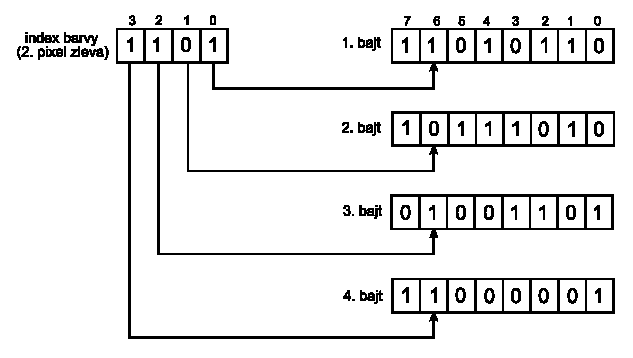
\includegraphics[width=10cm,height=5.4cm]{fig/pce_planar}
\caption{Planární způsob ukládání obrazových dat.\label{fig:vdc_planar}}
\end{center}
\end{figure}

V případě VDC HuC6270 systému NEC PCEngine index barvy uvádíme v rámci palety
určené ukazatelem v tabulce {\it BAT} nebo {\it SAT}. Každá z 16-ti palet (ať
už palet pro dlaždice pozadí, nebo palet pro sprajty) může obsahovat maximálně
16 barev, jejichž indexy zakódujeme pomocí 4 bitů. Pro uložení obrazových dat
zpracovávanhých VDC HuC6270 budou tedy potřeba 4 bitové roviny.

Vzory dlaždic pozadí jsou ve videopaměti reprezentovány jako 8 čtveřic bajtů
pro jednotlivé bitové roviny. Tyto čtveřice reprezentují jednotlivé řádky
vzoru. Každý vzor dlaždice pozadí ve videopaměti zabírá $8 * 8 * 4b = 256b / 8
= 32B$. VDC HuC6270 neočekává čtveřice bajtů ve videopaměti přímo za sebou, ale
proložené mezerou 16 bajtů (viz. obr.~\ref{fig:vdc_pat}). Více podrobností
lze nalézt např. v \cite{MacDonald02}.

\begin{figure}[ht]
\begin{center}
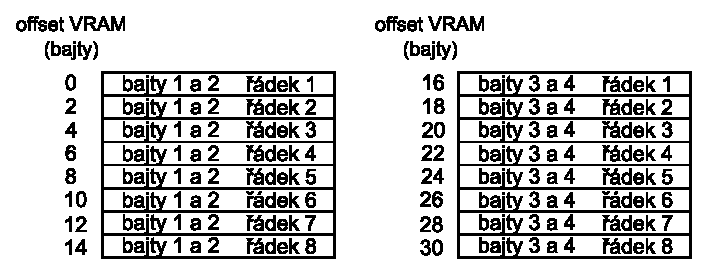
\includegraphics[width=11.5cm,height=4cm]{fig/pce_pixel}
\caption{Reprezentace vzoru dlaždice pozadí a vzoru sprajtu ve
videopaměti.\label{fig:vdc_pat}}
\end{center}
\end{figure}

Vzory sprajtů jsou ve videopaměti reprezentovány stejným způsobem jako vzory
dlaždic pozadí. Je však třeba vzít v úvahu několik drobných odlišností
týkajících se velikosti. Minimální velikost sprajtu je 16x16 pixelů, čtveřic
tedy není 8, ale 16 a pro jednotlivé řádky vzoru nejsou použity bajty ale
slova. Velikost jednoho vzoru sprajtu ve videopaměti je tedy $16 * 16 * 4b =
1024b / 8 = 128B$. VDC HuC6270 opět počítá s 16-ti bajtovým proložením ve
videopaměti (viz. obr.~\ref{fig:vdc_pat}).

Sprajty mohou navíc nabývat velikosti až 32x64 pixelů, což se řeší tak, že se
použijí sousední vzory sprajtů (ve skutečnosti se jedná přímo o maskování
pomocí atributů CGY a CGX). VDC HuC6270 se sprajtem větším než 16x16 pixelů
zachází z hlediska {\it SAT} úplně stejně, jako se sprajtem velkým 16x16 pixelů
(např. při použití atributu zrcadlového otočení v libovolné ose budou tedy
otočeny i příslušné okolní části sprajtu). Více podrobností lze nalézt např.
v~\cite{MacDonald02}.

% DMA

\subsubsection{Přímý přístup do paměti}\label{chap:spec_hw_vdc_dma}

VDC HuC6270 podporuje dva druhy přímého přístupu do paměti (Direct Memory
Access, DMA). Jedná se o:

\begin{itemize}
\item kopírování z videopaměti do videopaměti (dále jen VRAM/VRAM)
\item přesun z videopaměti do {\it SAT} (dále jen VRAM/{\it SAT})
\end{itemize}

Řízení DMA u VDC HuC6270 je prováděno pomocí čtveřice registrů {\sf DCR}, {\sf
SOUR}, {\sf DESR} a {\sf LENR}. Přenos je zahájen zápisem do registru {\sf
LENR}, který určuje délku bloku přenášeného z adresy uložené v registru {\sf
SOUR} na adresu uloženou v registru {\sf DESR}. Délka bloku může nabývat hodnot
0 pro 1B dlouhý blok, až po 65535 pro 64~KB dlouhý blok. Hodnoty jednotlivých
registrů slouží jako čítače a po dokončení se nenulují. Po ukončení libovolného
typu DMA přenosu může VDC HuC6270 vygenerovat přerušení IRQ1 (čtením ze
stavového registru VDC HuC6270 na logické adrese {\tt \$0000} jsme schopni
určit o jaký druh DMA se jednalo). Během DMA přenosu je stavový příznak VDC
HuC6270 \uv{čekání na CPU pro DMA (BSY)} nastaven na hodnotu \uv{1}.

% Registry

\subsubsection{Registry}\label{chap:spec_hw_vdc_regs}

VDC HuC6270 disponuje dvaceti registry o délce jednoho slova. K těmto registrům se
z CPU HuC6280 přistupuje pomocí tří speciálních instrukcí {\sc st0}, {\sc st1}
a {\sc st2} a vstupně-výstupní banky {\tt \$FF}
(viz.~\ref{chap:spec_hw_cpu_peripheral}). V té jsou namapovány tři důležité adresy
určené k čtení a zápisu do registrů VDC HuC6270. Jejich výčet a význam je uveden v
tabulce~\ref{tab:vdc_ffpage}. Detaily o významu jednotlivých bitů stavového
registru přístupného čtením log. adresy {\tt \$0000} lze nalézt např. v
\cite{MacDonald02}.

Zápis a čtení registrů VDC HuC6270 se provádí tak, že je zápisem spodních čtyř
bitů na logické adrese {\tt \$0000} nebo pomocí instrukce {\sc st0} zvolen
konkétní registr VDC HuC6270. Ten lze potom číst a zapisovat pomocí logických
adres {\tt \$0002} a {\tt \$0003}, nebo pomocí instrukcí {\sc st1} a {\sc st2}.
Dvojice adres pro zápis a čtení je použita, protože CPU HuC6280 je 8-mi bitový,
zatímco registry VDC HuC6270 jsou 16-ti bitové.

\begin{table}[ht]
\begin{center}
\begin{tabular}{|c|l|l|l|}
\hline
\textbf{Logická adresa} & \textbf{Operace} & \textbf{Bit} & \textbf{Význam} \\
\hline
	{\tt \$0000}
		& čtení
			& 7 & {\em nevyužito} \\
			& & 6 & čekání na CPU pro DMA (BSY) \\
			& & 5 & přerušení vertikální synchronizace (VD) \\
			& & 4 & přerušení \uv{konec DMA VRAM/VRAM} (DV) \\
			& & 3 & přerušení \uv{konec DMA VRAM/{\it SAT}} (DS) \\
			& & 2 & přerušení \uv{raster compare} (RR) \\
			& & 1 & přerušení přetečení sprajtů (OR) \\
			& & 0 & přerušení kolize sprajtu 0 (CR) \\
		& zápis
			& 7-5 & {\em nevyužito} \\
			& & 4-0 & offset registru VDC pro zápis/čtení \\
\hline
	{\tt \$0002}
		& čtení/zápis
		& 7-0 & méně významný bajt slova v registru VDC \\
\hline
	{\tt \$0003}
		& čtení/zápis
		& 7-0 & více významný bajt slova v registru VDC \\
\hline
\end{tabular}
\end{center}
	\caption{Adresy VDC HuC6270 ve vstupně-výstupní bance \$FF CPU
	HuC6280\label{tab:vdc_ffpage}}
\end{table}

Význam důležitých registrů je popsán v následujícím výčtu. Číslo uvedené za
slovem \uv{Registr} je offset registru, které se skutečně zapisuje na spodní
čtyři bity logické adresy {\tt \$0000}. Podrobné informace o jednotlivých
registrech lze nalézt např. v \cite{Schleussinger98}.

\begin{description}
\item[Registr {\tt \$00} {\sf MAWR}] (Memory Address Write) \\
	Čítač adresy při zápisu do videopaměti. Je nutné si uvědomit, že ačkoliv je
	VDC HuC6270 schopný adresovat 128~KB videopaměti, dostupných je v případě
	systému NEC PCEngine jen 64~KB, proto je poslední platnou adresou {\tt
	\$7FFF}.

\item[Registr {\tt \$01} {\sf MARR}] (Memory Address Read) \\
	Čítač adresy při čtení z videopaměti. Platí zde stejné adresní omezení jako
	v případě registru {\sf MAWR}.

\item[Registr {\tt \$02} {\sf VRR/VWR}] (VRAM Read/Write) \\
	Registr čtení/zápisu hodnoty z/do videopaměti na adrese udané hodnotou
	registru {\sf MARR}, příp. {\sf MAWR}. Při čtení více významného bajtu
	pomocí logické adresy {\tt \$0003} dochází k automatické inkrementaci
	registru {\sf MARR}. příp. {\sf MAWR}.

\item[Registr {\tt \$05} {\sf CR}] (Control Register) \\
	Konfigurační registr VDC HuC6270. Obsahuje bitové pole umožňující provádět
	řadu nastavení VDC HuC6270. Význam jednotlivých bitů (do kterého spadají
	příznaku) tohoto bitového pole je uveden v tabulce~\ref{tab:vdc_cr}. Význam
	jednotlivých příznaků uložených v tomto registru následuje:

	\begin{table}[ht]
	\begin{center}
	\begin{tabular}{|c|c|c|c|c|c|c|c|c|c|c|c|}
	\hline
	\textbf{Bit} & 15-13 & 12-11 & 10 & 9-8 & 7 & 6 & 5-4 & 3 & 2 & 1 & 0 \\
	\hline
	\textbf{Příznak} & ? & IW & ? & ? & BB & SB & ? & VB & RC & SO & SC \\
	\hline
	\end{tabular}
	\end{center}
		\caption{Význam bitů registru {\sf CR} VDC HuC6270\label{tab:vdc_cr}}
	\end{table}

	\begin{description}
	\item[IW] Hodnota těchto dvou bitů registru {\sf CR} určuje skok, o který
		se bude automaticky inkrementovat hodnota registru {\sf MAWR} po čtení
		významějšího slova (tj. čtení z logické adresy {\tt \$0003}). Hodnoty
		(decimálně):
		\begin{description}
		\item[{\tt 0}]: inkrementace o 1
		\item[{\tt 1}]: inkrementace o 32
		\item[{\tt 2}]: inkrementace o 64
		\item[{\tt 3}]: inkrementace o 128
		\end{description}

	\item[BB] Povolení/zákaz vykreslování roviny dlaždic pozadí.

	\item[SB] Povolení/zákaz vykreslování roviny sprajtů.

	\item[VB] Povolení/zákaz generování přerušení IRQ1 při \uv{vertical
		blanking}.

	\item[RC] Povolení/zákaz generování přerušení IRQ1 při \uv{raster
		compare}.

	\item[SO] Povolení/zákaz generování přerušení IRQ1 při překrytí sprajtů.

	\item[SC] Povolení/zákaz generování přerušení IRQ1 při kolizi sprajtu 0.
	\end{description}

\item[Registr {\tt \$06} {\sf RCR}] (Raster Compare) \\
	Obsah tohoto registru po součtu s číslem 64 určuje číslo řádku při kterém
	VDC HuC6270 vyvolá přerušení IRQ1 (pokud je toto povoleno 3 nejnižším bitem
	registru {\sf CR}).

\item[Registr {\tt \$07} {\sf BXR}] (Background Scroll X) \\
	Spodních deset bitů tohoto registru udává posun roviny dlaždic pozadí v ose
	X (je to offset v pixelech, nikoliv v počtu dlaždic jak mylně uvádí některé
	dokumenty).

\item[Registr {\tt \$08} {\sf BYR}] (Background Scroll Y) \\
	Spodních devět bitů tohoto registru udává posun roviny dlaždic pozadí v ose
	Y (opět jde o offset v pixelech).

\item[Registr {\tt \$09} {\sf MWR}] (Memory Width) \\
	Tento registr obsahuje bitové pole, které určuje velikost roviny dlaždic
	pozadí (ta může být větší než rozlišení obrazovky, čehož se často využívá
	při použití registrů {\sf BXR} a {\sf BYR}). Význam jednotlivých bitů v
	tomto bitovém poli je uveden v tabulce~\ref{tab:vdc_mwr}.

	\begin{table}[ht]
	\begin{center}
	\begin{tabular}{|l|l|l|l|}
	\hline
	\textbf{Bit} & \textbf{Význam} & \textbf{Hodnota} & \textbf{Šířka} \\
	\hline
	15-7 & {\em nevyužito} && \\
	6 & výška roviny dlaždic pozadí & 0 & 32 dlaždic \\
		& & 1 & 64 dlaždic \\
	5-4 & šířka roviny dlaždic pozadí & 00 & 32 dlaždic \\
		& & 01 & 64 dlaždic \\
		& & 10 & 128 dlaždic \\
		& & 11 & 128 dlaždic \\
	3-0 & {\em nevyužito} && \\
	\hline
	\end{tabular}
	\end{center}
		\caption{Význam bitů registru {\sf MWR} VDC HuC6270\label{tab:vdc_mwr}}
	\end{table}

\item[Registr {\tt \$0F} {\sf DCR}] (DMA Control) \\
	Tento registr slouží k řízení DMA přenosů. Význam jednotlivých bitů v tomto
	bitovém poli je uveden v tabulce~\ref{tab:vdc_dcr}. Bity 2 a 3 určují
	operaci na zdrojové/cílové adrese, která se bude vykonávat v každé iteraci
	blokového přenosu. Podrobnosti o DMA přenosech jsou uvedeny v
	sekci~\ref{chap:spec_hw_vdc_dma}.

	\begin{table}[ht]
	\begin{center}
	\begin{tabular}{|l|l|l|l|}
	\hline
	\textbf{Bit} & \textbf{Význam} & \textbf{Hodnota} & \textbf{Operace} \\
	\hline
	15-5 & {\em nevyužito} && \\
	4 & DSR DMA (opakování DMA přenosu z VRAM do {\em SAT}) && \\
	3 & Operace aplikovaná na cílovou adresu & 0 & snížení o 1 \\
		& & 1 & zvýšení o 1 \\
	2 & Operace aplikované na zdrojovou adresu & 0 & snížení o 1 \\
		& & 1 & zvýšení o 1 \\
	1 & Povolení/zákaz přerušení \uv{konec DMA VRAM/VRAM} && \\
	0 & Povolení/zákaz přerušení \uv{konec DMA VRAM/{\it SAT}} && \\
	\hline
	\end{tabular}
	\end{center}
		\caption{Význam bitů registru {\sf DCR} VDC HuC6270\label{tab:vdc_dcr}}
	\end{table}

\item[Registr {\tt \$10} {\sf SOUR}] (DMA Source Address) \\
	Tento registr slouží k nastavení zdrojové adresy DMA přenosu.

\item[Registr {\tt \$11} {\sf DESR}] (DMA Destination Address) \\
	Tento registr slouží k nastavení cílové adresy DMA přenosu.

\item[Registr {\tt \$12} {\sf LENR}] (DMA Block length Address) \\
	Tento registr slouží k nastavení délky přenášeného bloku při DMA přenosu.
	Zápis do tohoto registru automaticky zahajuje DMA přenos.

\item[Registr {\tt \$13} {\sf SATB}] (Sprite Attribute Table) \\
	Tento registr obsahuje ukazatel na počátek tabulky {\em SAT} ve
	videopaměti.
\end{description}

% Preruseni

\subsubsection{Přerušení}\label{chap:spec_hw_vdc_irq}

VDC HuC6270 může v závislosti na nastavení registrů {\sf CR} a {\sf DCR}
generovat přerušení IRQ1 v řadě případů. Tyto případy lze snadno odlišit pomocí
příznaků přerušení ve stavovém registru VDC HuC6270, který lze číst na logické
adrese {\tt \$0000}.

Významná přerušení, která může VDC HuC6270 generovat jsou uvedena v
následujícím výčtu. Pro přehlednost jsou přerušení uvedena pod názvem
příslušných příznaků stavového registru VDC HuC6270.

\begin{description}
\item[VD] (Vertical Blanking) \\
	Toto přerušení je generováno při {\em vertikální synchronizaci}. Používá se k
	jednoduchému synchronizování programového kódu a vykreslování obrazu.

\item[DV] (VRAM to VRAM DMA Transfer Completion) \\
	Toto přerušení je generováno při dokončení operace DMA kopírování z
	videopaměti do videopaměti (VRAM/VRAM).

\item[DS] (VRAM to SAT DMA Transfer Completion) \\
	Toto přerušení je generováno při dokončení operace DMA přesun z videopaměti
	do {\it SAT}.

\item[RR] (Raster Compare) \\
	Toto přerušení je generováno, když interní čítač řádek obrazovky nabyde
	hodnoty registru {\sf RCR} zvětšené o číslo 64. \cite{Schleussinger98}

\item[OR] (Sprite Overflow) \\
	Toto přerušení nastává pokud je v aktuálně vykreslované řádce více než 16
	sprajtů.

\item[CR] (Sprite 0 Collision) \\
	Toto přerušení nastává v případě, kdy se netransparentní pixel sprajtu s
	pořadovým číslem 0 (tj. prvního záznamu v tabulce {\it SAT}) překryje s
	netransparentním pixelem kteréhokoliv jiného sprajtu.
\end{description}

%
% VCE
%

\subsection{VCE}\label{chap:spec_hw_vce}

Video Color Encoder (VCE), neboli enkodér barev nese označení HuC6260 a
obstarává systému NEC PCEngine správu barev. Pomocí registrů VCE je možné měnit
barvy ve všech 32 paletách (16 palet pro dlaždice pozadí a 16 palet pro
sprajty).

% Palety

\subsubsection{Palety}\label{chap:spec_hw_vce_palette}

Jak již bylo uvedeno dříve, VDC HuC6270 a VCE HuC6260 pracují celkem s 512-ti
barvami uloženými v barevné tabulce. Prvních 256 záznamů je určeno výhradně pro
vykreslování dlaždic pozadí a zbývajících 256 záznamů, pak výhradně pro
vykreslování sprajtů. Logicky jsou barvy v tabulce uspořádány do dvou skupin
16-ti palet, kde každá paleta obsahuje 16 barev. Tyto palety jsou odkazovány
přímo v ukazatelích z atributových tabulek {\it BAT} a {\it SAT} spravovaných
VDC HuC6270.

Jednotlivé záznamy tabulky barev jsou slova obsahující barevnou informaci.
Tvar jednoho záznamu z barevné tabulky je uveden v tabulce~\ref{tab:vce_color}.
Indexace barev probíhá v rámci celé tabulky 9-ti bitovým indexem barvy (logické
rozdělení na palety a skupiny palet je vnímáno pouze při práci s tabulkami {\it 
BAT} a {\it SAT} v rámci VDC HuC620.

\begin{table}[ht]
\begin{center}
\begin{tabular}{|l|l|}
\hline
\textbf{Bit} & \textbf{Význam} \\
\hline
15-9 & {\em nevyužito} \\
8-6 & zelená \\
5-3 & červená \\
2-0 & modrá \\
\hline
\end{tabular}
\end{center}
\caption{Tvar záznamu v barevné tabulce VCE
	HuC6260\label{tab:vce_color}}
\end{table}

Palety obsahují několik speciálních barev, při jejichž použití musíme očekávat
jiné chování vykreslovacích mechanismů. Tyto speciální barvy jsou:

\begin{description}
\item[transparentní barva] - transparentní barvu mají pixely (dlaždice pozadí
	nebo sprajtu), které nemají být vykresleny. V případě dlaždice pozadí bude
	na jejich místě vykreslena {\em barva pozadí}, v případě sprajtu barva
	pixelu dlaždice pozadí ležícím v místě transparentního pixelu sprajtu
	(případně opět {\em barva pozadí}, pokud je i pixel dlaždice pozadí
	transparentní). Transparentní barva je umístěna na indexu 0 ve všech
	paletách dlaždic pozadí i sprajtů.

\item[barva pozadí] - barva, která je vykreslena na místě \uv{pod}
	transparentním pixelem dlaždice pozadí. Tato barva je umístěna v 0-té
	paletě pro dlaždice pozadí na indexu 0 (tato barva je vlastně transparentní
	barvou pro všechny palety dlaždic pozadí). Barvu na indexu 0 všech
	ostatních palet pro dlaždice pozadí není možné zobrazit.

\item[barva přesahu] - barva, která je vykreslována zpravidla mimo plochu
	aktivního obrazu. Jedinný případ, kdy je tato barva zobrazena na obrazovce
	je, když je pomocí registru {\sf CR} VDC HuC6270 zakázáno vykreslování obou
	rovin (dlaždic pozadí i sprajtů). Jedná se o barvu na indexu 0 v 0-té
	paletě pro sprajty. Barvu na indexu 0 barvu všech ostatních palet pro
	sprajty též není možné zobrazit.
\end{description}

% Registry

\subsubsection{Registry}\label{chap:spec_hw_vce_regs}

VCE mapuje své registry do adresního prostoru CPU HuC6280 pomocí čtveřice adres
v rámci stránky {\tt \$FF} (viz.~\ref{chap:spec_hw_cpu_peripheral}). Jejich výčet a
význam je uveden v tabulce~\ref{tab:vce_ffpage}. Práce s VCE HuC6260 je v
mnohém analogická s prací VDC HuC6270.

\begin{table}[ht]
\begin{center}
\begin{tabular}{|c|l|l|l|}
\hline
\textbf{Logická adresa} & \textbf{Význam} \\
\hline
	{\tt \$0402} & Index barvy v tabulce (méně významný bajt) \\
	{\tt \$0403} & Index barvy v tabulce (více významný bajt) \\
	{\tt \$0404} & Data (méně významný bajt) \\
	{\tt \$0405} & Data (více významný bajt) \\
\hline
\end{tabular}
\end{center}
	\caption{Adresy VCE HuC6260 ve vstupně-výstupní bance \$FF CPU
	HuC6280\label{tab:vce_ffpage}}
\end{table}

%
% PSG
%

\subsection{PSG}\label{chap:spec_hw_psg}

Programmable Sound Generator (PSG), tedy programovatelný generátor
zvuku, je jedno z periferních zařízení CPU HuC6280 osazené na stejném čipu.
Podrobně se jím zabývá např.~\cite{Clifford}.

PSG je vybaven šesti kanály, které jsou primárně určeny pro přehrávání 32
bajtových lineárních samplů s rozlišením 5 bitů. Některé kanály mohou být
využity k frekvenční modulaci\footnote{Možnost měnit aktuální nosnou frekvenci
přehrávaného signálu pomocí modulační amplitudy.} pomocí nízkofrekvenčního
oscilátoru (Low Frequency Oscillator, LFO), či generování bílého
šumu\footnote{Náhodný signál se stejným výkonem v pásmech se shodnou šířkou.
Využívá se k neumělé syntetizaci zvuku perkusí apod.} (White Noise). Každý z
kanálů může být také přepnut do módu přímého přístupu k datům (Direct Data
Access, DDA), kdy je zvuk programován přímo CPU HuC6280, což dovoluje např.
jednoduchou syntézu zvuku. Možnosti jednotlivých kanálů PSG jsou uvedeny v
tabulce~\ref{tab:psg_chan}.

V případě nastavení módu frekvenční modulace pro kanál 0 bude kanál 1 vždy
automaticky ztlumen.

\begin{table}[ht]
\begin{center}
\begin{tabular}{|c|l|}
\hline
\textbf{Kanál} & \textbf{Dostupné režimy} \\
\hline
	0 & samply, frekvenční modulace (podle kanálu 1), DDA \\
	1 & samply, frekvenční modulace (kanálu 0), DDA \\
	2 & samply, DDA \\
	3 & samply, DDA \\
	4 & samply, bílý šum, DDA \\
	5 & samply, bílý šum, DDA \\
\hline
\end{tabular}
\end{center}
	\caption{Možnosti jednotlivých kanálů PSG\label{tab:psg_chan}}
\end{table}

Ke zprocesování dat využívá PSG stejný zdroj hodin jako CPU HuC6280. Jedná se o
hodiny pevně nastavené na hodnotu 3.58~MHz nezávisle na stavu skrytého registru
{\sf CS} CPU HuC6280.

% Registry

\subsubsection{Registry}\label{chap:spec_hw_psg_regs}

Podobně jako VDC HuC6270, nebo VCE HuC6260 i PSG mapuje své registry do
adresního prostoru CPU HuC6280. Jedná se o deset adres v rámci stránky {\tt
\$FF} (viz.~\ref{chap:spec_hw_cpu_peripheral}). Jejich výčet a význam je uveden v
tabulce~\ref{tab:psg_ffpage}, kde jsou ve spodní části tabulky oddělené čarou
uvedeny registry ovlivněné hodnotou zapsanou na adresu {\tt \$8000}. Všechny
registry PSG jsou 8-mi bitové.

Nastavení hodnot registrů ovládajících režim (frekvenční modulace, generování
bílého šumu) u kanálu, kde tento režim není dostupný, bude PSG ignorováno.

\begin{table}[ht]
\begin{center}
\begin{tabular}{|c|l|l|l|}
\hline
\textbf{Logická adresa} & \textbf{Význam} \\
\hline
	{\tt \$0800} & Výběr kanálu (Channel Select) \\
	{\tt \$0801} & Globální vyvážení hlasitosti (Global Balance) \\
\hline
	{\tt \$0802} & Jemné nastavení frekvence (Fine Frequency Adjust) \\
	{\tt \$0803} & Hrubé nastavení frekvence (Rough Frequency Adjust) \\
	{\tt \$0804} & Režim kanálu (Channel Mode) \\
	{\tt \$0805} & Vyvážení hlasitosti (Channel Balance) \\
	{\tt \$0806} & Data \\
	{\tt \$0807} & Povolení a frekvence bílého šumu (Noise Control) \\
	{\tt \$0808} & Frekvence oscilátoru modulace (LFO Frequency) \\
	{\tt \$0809} & Povolení a ovládání oscilátoru modulace (LFO Control) \\
\hline
\end{tabular}
\end{center}
	\caption{Adresy PSG ve vstupně-výstupní bance \$FF CPU
	HuC6280\label{tab:psg_ffpage}}
\end{table}

\begin{description}
\item [Registr {\tt \$0800}] (Channel Select) \\
	Nastavením spodních 2 bitů se určuje, který z kanálů PSG bude použit
	při zápisech/čteních registrů {\tt \$0802} - {\tt \$0809}.

\item [Registr {\tt \$0801}] (Global Balance) \\
	Hodnota tohoto registru určuje globální hlasitost pro levý a pravý kanál v
	mezích hodnot 0-15. Pro nastavení globální hlasitosti pravého kanálu slouží
	spodní 4 bity, pro nastavení globální hlasitosti levého kanálu pak
	následující 4 bity. Tato hlasitost je aplikována až po smíšení všech kanálů
	v jejich konkrétních hlasitostech.

\item [Registry {\tt \$0802}] (Fine Frequency Adjust) a
	{\tt \$0803} (Rough Frequency Adjust) \\
	Frekvence je v případě PSG 12-ti bitové číslo. Spodní 4 bity registru {\tt
	\$0803} představují vrchní 4 bity a hodnota registru {\tt \$0802}
	zbývajících 8 bitů tohoto čísla. Pro převod na Hz lze použít následující
	vztah: $$ f = \frac{3580000}{32 * 12bit} Hz $$ což je dáno způsobem práce
	s frekvencí v režimu přehrávání samplů. V tomto režimu se jedná o ukazatel,
	který je dekrementován o 1 celkem 3580000-krát za sekundu a ukazuje přímo
	do dat samplu.

\item [Registr {\tt \$0804}] (Channel Control) \\
	Tento registr slouží jako bitové pole určené ke konfiguraci parametrů
	zvoleného kanálu. Význam jednotlivých bitů je popsán v
	tabulce~\ref{tab:psg_cr}.

	\begin{table}[ht]
	\begin{center}
	\begin{tabular}{|l|l|}
	\hline
	\textbf{Bit} & \textbf{Význam} \\
	\hline
		7 & Kanál zapnut/vypnut \\
		6 & DDA režim zapnut/vypnut \\
		5 & {\em nevyužito} \\
		4-0 & Celková hlasitost kanálu \\
	\hline
	\end{tabular}
	\end{center}
		\caption{Význam bitů registru {\tt \$0804} PSG\label{tab:psg_cr}}
	\end{table}

\item [Registr {\tt \$0805}] (Channel Balance) \\
	Tento registr slouží k nastavení vyvážení hlasitosti zvoleného kanálu.
	Pracuje analogicky s registrem {\tt \$0801}.

\item [Registr {\tt \$0806}] (Data) \\
	Spodních 5 bitů tohoto registru slouží k zápisu dat na zvolený kanál.
	Chování registru je rozdílné podle zvoleného režimu kanálu (viz. bity 7 a 6
	registru {\tt \$0804}).

	V běžném případě se do tohoto registru zapisují data samplu. V případě, že
	je na kanálu povoleno DDA, pak jsou data zapsaná do tohoto registu přímo
	mixována s ostatními kanály. V případě, že je zvolen kanál 1, je neaktivní
	a DDA je vypnuto, slouží tento registr k zápisu modulační vlny (více viz.
	\cite{Clifford}).

\item [Registr {\tt \$0807}] (Noise Control) \\
	Tento registr slouží k zapnutí a vypnutí generátoru bílého šumu a nastavení
	jeho frekvence. Použití tohoto registru má význam pouze v případě kanálů 4
	a 5. Registr je uspořádán jako bitové pole s bity významu popsaného v
	tabulce~\ref{tab:psg_noise}. Frekvence bílého šumu nastavovaná pomocí
	spodních 5-ti bitů je vyjádřena vzorcem (podrobnosti o původu vzorce lze
	nalézt v \cite{Clifford}): $$ f = \frac{3580000}{64 * 5bit} Hz $$

	\begin{table}[ht]
	\begin{center}
	\begin{tabular}{|l|l|}
	\hline
	\textbf{Bit} & \textbf{Význam} \\
	\hline
		7 & Bílý šum zapnut/vypnut \\
		6-5 & {\em nevyužito} \\
		4-0 & Frekvence šumu \\
	\hline
	\end{tabular}
	\end{center}
		\caption{Význam bitů registru {\tt \$0807} PSG\label{tab:psg_noise}}
	\end{table}

\item [Registr {\tt \$0808}] (LFO Frequency) \\
	V případě, že je kanál 0 v režimu frekvenční modulace, slouží tento registr
	u kanálu 1 k modelování frekvence modelovací vlny (definované registry {\tt
	\$0802} a {\tt \$0803} při vybraném kanálu 1. Frekvence daná tam uloženým
	12-ti bitovým číslem je vynásobena frekvencí LFO uloženou v tomto registru
	před dalším zpracováním.

\item [Registr {\tt \$0809}] (LFO Control) \\
	Tento registr slouží k ovládání parametrů frekvenční modulace kanálu 0
	kanálem 1. Jedná se o bitové pole, kde význam jednotlivých bitů je uveden v
	tabulce~\ref{tab:psg_lfo}. Více informací o programování oscilátoru
	frekvenční modulace je uvedeno v \cite{Clifford}.

	\begin{table}[ht]
	\begin{center}
	\begin{tabular}{|l|l|}
	\hline
	\textbf{Bit} & \textbf{Význam} \\
	\hline
		7 & Oscilátor modulace zapnut/vypnut \\
		6-2 & {\em nevyužito} \\
		1-0 & Režim oscilátoru modulace \\
	\hline
	\end{tabular}
	\end{center}
		\caption{Význam bitů registru {\tt \$0809} PSG\label{tab:psg_lfo}}
	\end{table}

\end{description}

%
% ROM
%

\subsection{Obraz ROM}\label{chap:spec_hw_rom}

Obraz ROM je binární otisk obsahu paměti v paměťovém modulu na čipové kartě
HuCard do souboru. Lze jej pořídit pomocí speciálního zařízení (např. PCE Pro
32M na obr.~\ref{fig:pce_pcepro32}), které sekvenčně adresuje a čte jednotlivé
bloky paměti připojené čipové karty HuCard a pomocí speciálního software
komunikujícího se zařízením pomocí standardního rozhraní (USB, paralelní port)
je ukládá do souboru na disku PC.

\begin{figure}[ht]
\begin{center}
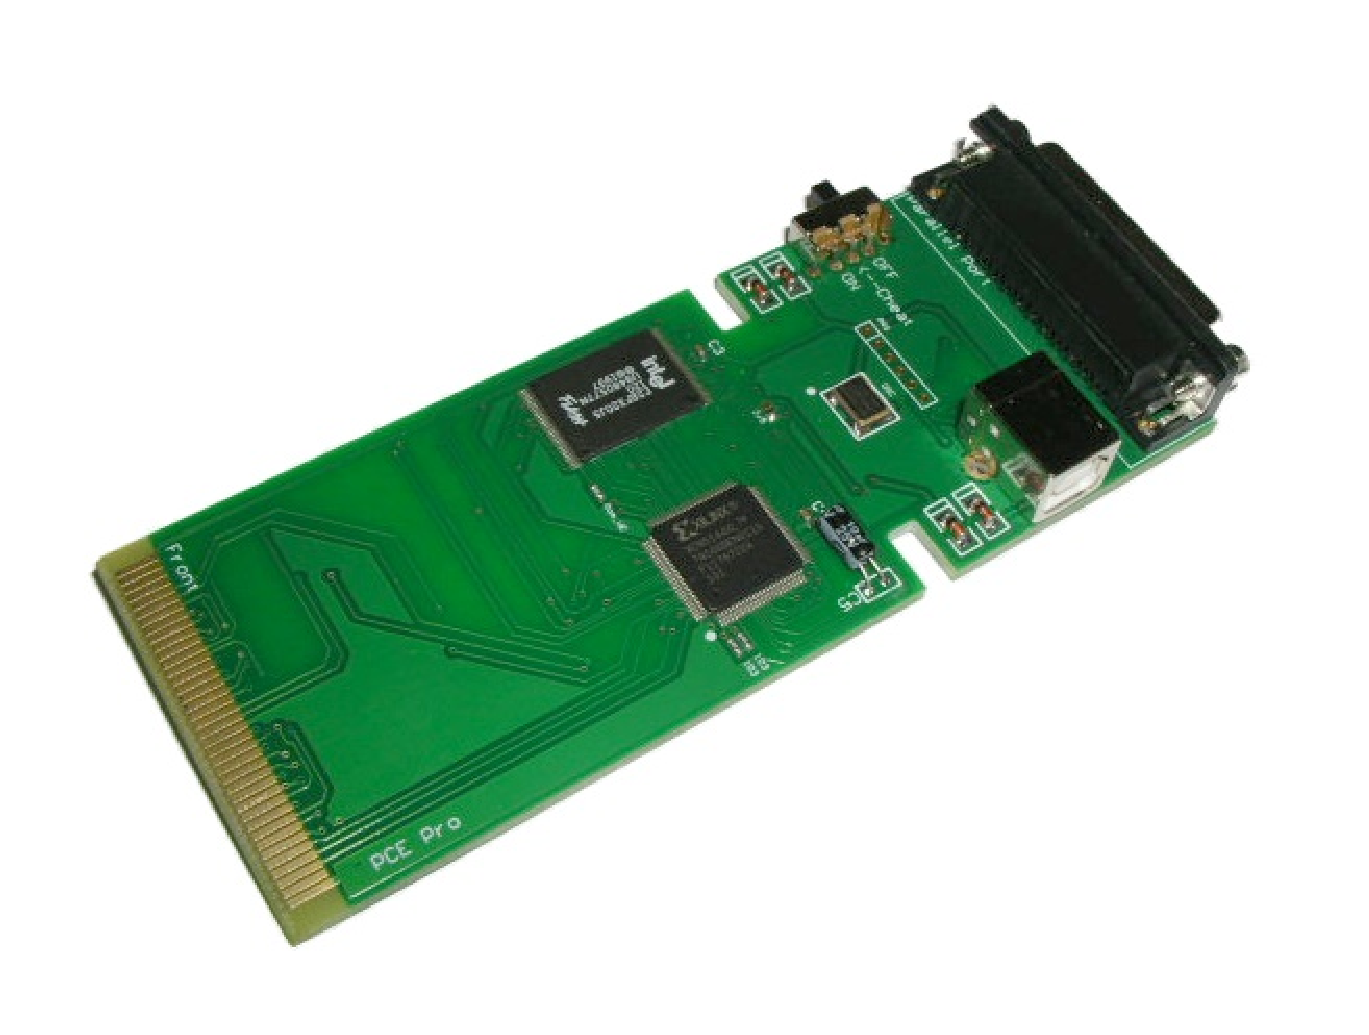
\includegraphics[width=6cm]{fig/pce_pcepro32}
\caption{PCE Pro 32M\label{fig:pce_pcepro32}}
\end{center}
\end{figure}

V nepříliš široké komunitě zabývající se emulací systému NEC PCEngine se
ustálil formát souboru s obrazem ROM použitý prvním emulátorem tohoto systému
(MagicEngine,~\cite{wwwMagicEngine}). Tento formát se vyznačuje absencí
jakýchkoliv metadat, kromě volitelné 512 bajtové hlavičky v úvodu souboru,
kterou lze snadno detekovat lichým počtem 512 bajtových bloků v souboru s
obrazem ROM.

Speciálním případem obrazu ROM jsou poměrně často používané obrazy o velikosti
384~KB. Tyto obrazy musí být rozděleny na dvě části umístěné v paměti ROM podle
schématu naznačeného v tabulce~\ref{tab:rom_split}.

\begin{table}[h!]
\begin{center}
\begin{tabular}{|l|l|l|}
\hline
\textbf{Offset v souboru} & \textbf{Délka} & \textbf{Offset v ROM} \\
\hline
	{\tt \$00000} & {\tt \$40000} & {\tt \$00000} \\
	{\tt \$40000} & {\tt \$20000} & {\tt \$80000} \\
\hline
\end{tabular}
\end{center}
	\caption{Schéma rozdělení 384~KB obrazů ROM\label{tab:rom_split}}
\end{table}

Maximální velikost paměťového modulu v čipové kartě HuCard je v základní
specifikaci omezena na 1~MB, minimální velikost není určena.

% -----------------------------------------------------------------------------
% Software NEC PCEngine
% -----------------------------------------------------------------------------

\section{Software}\label{chap:spec_sw}

Za dobu působení společnosti NEC v oblasti videoherního průmyslu, od roku 1987
do roku 1998, vznikla pro systém NEC PCEngine řada titulů. Jak samotný účel
systému předurčuje, majoritní většina byly herní programy. Kromě původních
titulů se společnost NEC snažila získat uživatele videoherních systémů na svou
stranu vydáním některých titulů, které se proslavily na systému Nintendo NES,
jako např. {\em Castlevania} nebo {\em StreetFighter}. Řada titulů vydaných
právě pro NEC PCEngine je přehledně katalogizována na~\cite{wwwPceCP}.

%%%%%%%%%%%%%%%%%%%%%%%%%%%%%%%%%%%%%%%%%%%%%%%%%%%%%%%%%%%%%%%%%%%%%%%%%%%%%%%
% bc.tex - Bachelor thesis                                                    %
% Subject: bc_emu - portable video game emulator                              %
% Chapter: Existujici implementace                                            %
% Author: Ondrej Balaz <ondra@blami.net>                                      %
%%%%%%%%%%%%%%%%%%%%%%%%%%%%%%%%%%%%%%%%%%%%%%%%%%%%%%%%%%%%%%%%%%%%%%%%%%%%%%%

\chapter{Existující implementace}\label{chap:exist}

I přes to, že systém NEC PCEngine nikdy nedosáhl podobné popularity a rozšíření
ve světe, jako jiné videoherní konzole stejné generace (Nintendo Famicom, Sega
Master System, Atari 7800), vzniklo několik jeho emulátorů. Jejich existence
značně usnadňuje vývoj a lazení nového emulátoru. Kromě toho, že mohou být
použity jako prostředek pro ověření funkčnosti v případě absence skutečného,
dnes již nedostupného, hardware systému NEC PCEngine, je řada z nich šířena i
ve zdrojové podobě jako svobodný software, což umožňuje studovat jak
specifikaci systému, tak i způsob jakým jejich autoři vyřešili vlastní
implementaci jeho jednotlivých částí.

V úvodní sekci~\ref{chap:exist_listing} této kapitoly je nastíněna situace v
oblasti emulace systému NEC PCEngine a jsou představeny některé existující
implementace emulátorů. Sekce~\ref{chap:exist_summary} shrnuje přednosti a
nedostatky těchto implementací a na jejich základě nastiňuje směr pro další
analýzu, návrh a implementaci vlastního emulátoru.

% -----------------------------------------------------------------------------
% Přehled emulátorů NEC PCEngine
% -----------------------------------------------------------------------------

\section{Přehled emulátorů NEC PCEngine}\label{chap:exist_listing}

Většina emulátorů systému NEC PCEngine vznikla v letech 1995-2001, hlavně pro
osobní počítače s operačními systémy Microsoft DOS a Microsoft Windows. V
následujícím přehledu jsou uvedeny pouze tři nejpoužívanější, aktivně udržované
a vyvíjené emulátory. Další, které většinou nejsou zdaleka tak kompletní z
hlediska funkčnosti a kompatibility se zveřejněnými čipovými kartami HuCard,
nebo je jejich kód zastaralý a jsou v dnešních podmínkách nepoužitelné, lze
nalézt např. na~\cite{wwwEmulatorZone}.

% MagicEngine

\subsection{MagicEngine}

MagicEngine~\cite{wwwMagicEngine} je komerční emulátor systému NEC PCEngine.
Podporuje emulaci všech verzí systému včetně řady rozšíření (např. CD-ROM
mechanika). Emulace je v podání tohoto emulátoru velice přesná, rychlá a bez
problému je možné spustit většinu obrazů zveřejněných na čipových kartách
HuCard, včetně těch, které využívají nestandardního chování systému.

Podporovány jsou platformy Microsoft DOS (jen starší verze emulátoru),
Microsoft Windows a Apple MacOS X. Program disponuje vlastním jednoduchým
grafickým uživatelským rozhraním. Nároky na hardware jsou poměrně vysoké a při
použití pod operačním systémem Windows vyžaduje MagicEngine grafickou
akceleraci pomocí DirectX nebo OpenGL. V současné době se jedná o
nejpopulárnější emulátor NEC PCEngine pro Microsoft Windows.

Přesto, že autoři MagicEngine významným dílem přispěli ke zdokumentování
architektury NEC PCEngine a zveřejnili řadu nástrojů pro vývoj programů s tímto
systémem kompatibilních, zdrojový kód MagicEngine není otevřený, což znemožňuje
zásahy kýmkoliv jiným než autory.

\subsubsection*{Klíčové vlastnosti}

\begin{itemize}
\item vysoká přensnost emulace
\item podpora všech verzí a rozšíření systému
\item kompatibilita s většinou čipových karet HuCard
\end{itemize}

% Ootake

\subsection{Ootake}

Ootake~\cite{wwwOotake} je emulátor systému NEC PCEngine od japonského autora
Nakamura Kitao. Podobně jako MagicEngine podporuje Ootake všechny verze systému
včetně řady rozšíření. Autor se speciálně věnuje problematice dosažení stejného
pocitu ze hry\footnote{Např. poměrně složitě implementuje zpracování vstupu
z herního ovladače tak, aby bylo kompenzováno zpoždění způsobené obsluhami
operačního systému.} jako na originálním hardware, takže je emulátor velice
přesný i po stránce zpracování vstupu apod. Množina podporovaných titulů je o
něco menší než v případě MagicEngine.

Ootake je napsán výhradně pro platformu Microsoft Windows v jejímž duchu se
také nese uživatelské rozhraní programu. Hardwarové nároky Ootake jsou poměrně
vysoké, emulátor vyžaduje grafickou akceleraci pomocí DirectX a procesor s
rychlostí cca 1.6GHz pro plynulý běh herních programů.

Zdrojový kód emulátoru Ootake je veřejně přístupný a šířen pod licencí GNU/GPL.
Vzhledem k tomu, že je program vyvíjen bez ohledu na přenositelnost kódu, na
řadě míst se prolíná kód zajišťující logiku emulace a specifický kód pro
uživatelské rozhraní v Microsoft Windows. Kód je z důvodu přesnosti emulace
protkán řadou optimalizací a jeho čitelnost navíc ztěžuje fakt, že veškeré
komentáře jsou psány v japonštině.

\subsubsection*{Klíčové vlastnosti}

\begin{itemize}
\item vysoká přesnost emulace s ohledem na pocit ze hry
\item podpora všech verzí a rozšíření systému
\item otevřený zdrojový kód
\end{itemize}

% Mednafen

\subsection{Mednafen}

Mednafen~\cite{wwwMednafen} je emulátor několika populárních videoherních
systémů mezi nimiž je i systém NEC PCEngine. Emulace NEC PCEngine v rámci
tohoto programu využívá několika společných komponent s emulátorem systému NEC
PC FX32, který je nástupcem NEC PCEngine. Stejně jako v předchozích případech
je podporována řada rozšíření. I přes některé nepřesnosti časování v emulaci je
celková přesnost emulace vysoká. Součástí programu je podpora hry více hráčů na
jedné konzoli přes TCP/IP (vzdálený herní ovladač), nebo vestavěný ladicí
nástroj, který umožňuje krokovat běžící herní program a sledovat obsah
významných oblastí paměti a registrů.

Program je psán přenositelně a je prokazatelně možné ho sestavit a používat na
platformách GNU/Linux, FreeBSD, Apple MacOS X a Microsoft Windows. Uživatelské
rozhraní programu je zajištěno pomocí přenositelné knihovny pro uživatelská
rozhraní libSDL. Hardwarové nároky na plynulou emulaci jsou oproti předchozím
řešením nižší.

Mednafem má otevřený zdrojový kód šířený pod licencí GNU/GPL. Je psán v jazyce
C++ s důrazem na přenositelnost, hlavně mezi platformami GNU/Linux a Microsoft
Windows. Nepočítá se však s přenositelností na platformy, kde není dostupná
knihovna libSDL, která je pevnou součástí programového kódu. Stejně tak
jednotlivé emulátory podporovaných systémů nepoužívají žádné společné rozhraní,
které by umožňovalo program jednoduše rozšířit.

\subsubsection*{Klíčové vlastnosti}

\begin{itemize}
\item podpora dalších videoherních systémů
\item integrovaný nástroj pro lazení emulovaných programů
\item podpora hry více hráčů po síti TCP/IP
\item otevřený zdrojový kód
\item přenositelnost
\end{itemize}

% -----------------------------------------------------------------------------
% Shrnuti
% -----------------------------------------------------------------------------

\section{Shrnutí}\label{chap:exist_summary}

Většina existujících implementací emulátoru NEC PCEngine (včetně řady těch,
které nejsou v předchozím výčtu uvedeny) jsou jednoúčelové programy soustředící
se výhradně na emulaci tohoto systému, případně jeho dalších variant a
rozšíření.

Jistě pozitivní stránkou tohoto přístupu je v některých případech vysoká
přesnost a kvalita emulace, protože se autor nemusí soustředit na řadu dalších
podporovaných videoherních systémů. Na druhou stranu je množina opravdu
nezapomenutelných a populárních herních titulů pro jednotlivé videoherní
systémy poměrně malá\footnote{Velice populární japonská série herních titulů
Final Fantasy vydávaná společnosti Square Enix má v současné době více než 13
dílů, které vyšly střídavě pro 12 různých typů videoherních systémů s průměrnou
bilancí 1-2 díly na jeden typ videoherního systému.} a uživatelé často
používají více emulátorů několika různých systému. Jsou tak nuceni používat
více jednoúčelových programů s různým způsobem ovládání a chováním i přesto, že
jejich úkol je z uživatelského pohledu stejný.

\uv{Slabinou} existujících implementací je také poměrně malá množina
podporovaných platforem. Jak již bylo uvedeno, většina emulátorů systému NEC
PCEngine vznikla v letech 1995-2001, tedy v období kdy poměrně vysokým nárokům
na výkon při provádění emulace dostačovaly prakticky jen osobní počítače a v
oblasti operačních systémů nebyl např. GNU/Linux zdaleka tak populární jako
Microsoft DOS nebo Microsoft Windows.

V současné době existuje řada videoherních handheldů\footnote{Přenosné kapesní
videoherní konzole vybavené displejem a ovládacími prvky herního ovladače,
často napájené z baterií, např. Sony Playstation Portable, Nintendo DS nebo
Gamepark Wiz.}, chytrých mobilních telefonů\footnote{Mobilní telefony vybavené
operačním systémem umožňujícím instalaci a spouštění dalších programů, např.
Nokia Series60 s operačním systémem Symbian nebo telefony HTC s operačními
systémy Google Android nebo Microsoft Windows Mobile} a kapesních počítačů,
které mohou výkonem směle konkurovat tehdejším osobním počítačům, nikoliv však
těm dnešním, což je jeden z důvodů proč právě tato zařízení jsou zajímavou,
platformou pro emulátory starších videoherních systémů. Většina existujících
emulátorů ale stěží počítá s přenositelností na jiné operační systémy než je
Microsoft Windows, natož na tato zařízení.

Kromě slabin existujících implmentací ale existují i jejich přednosti. Nejvíce
inspirativní je v této oblasti poslední zmíněný emulátor Mednafen, který
implementuje přenositelné uživatelské rozhraní pomocí knihovny libSDL a
obsahuje podporu pro lazení emulovaného programu, nebo hru více hráčů po síti
TCP/IP.

Při následující analýze a návrhu vlastního emulátoru je kladen důraz na
potlačení uvedených nedostatků při zachování předností existujících řešení.

Emulátor bude navržen modulárně, aby bylo v budoucnu snadné ho rozšířit
o podporu emulace dalších videoherních systémů při zachování společného
ovladání. Stejně tak podpora platforem nebude způsobem implementace omezena
pouze na operační systémy osobních počítačů.

%%%%%%%%%%%%%%%%%%%%%%%%%%%%%%%%%%%%%%%%%%%%%%%%%%%%%%%%%%%%%%%%%%%%%%%%%%%%%%%
% bc.tex - Bachelor thesis                                                    %
% Subject: bc_emu - portable video game emulator                              %
% Chapter: Analyza a navrh                                                    %
% Author: Ondrej Balaz <ondra@blami.net>                                      %
%%%%%%%%%%%%%%%%%%%%%%%%%%%%%%%%%%%%%%%%%%%%%%%%%%%%%%%%%%%%%%%%%%%%%%%%%%%%%%%

\chapter{Analýza a návrh}\label{chap:anal}

Analýza a návrh, jimž se věnuje tato kapitola, jsou obecně nejdůležitější fází
vývojového procesu. V sekcích~\ref{chap:anal_emulation}
a~\ref{chap:anal_techniques} jsou popsány nejčastější používané techniky emulace
jednotlivých součástí videoherních systémů s ohledem na specifikaci systému NEC
PCEngine (viz. kapitola~\ref{chap:spec}).

Na jejich základě a v závislosti na požadavcích vyplývajících z rešerše
existujících implementací (viz. kapitola~\ref{chap:exist}), shrnutých v
sekci~\ref{chap:anal_requirements}, byla pro následnou implementaci
modulárního, přenositelného emulátoru navržena architektura, kterou popisuje
sekce~\ref{chap:anal_architecture}.

% -----------------------------------------------------------------------------
% Emulace
% -----------------------------------------------------------------------------

\section{Emulace}\label{chap:anal_emulation}

Emulace je v oblasti počítačové vědy proces, kdy program zvaný emulátor co
nejpřesněji napodobuje interní chování emulovaného zařízení. Z hlediska
uživatele tak navozuje dojem práce s tímto zařízením. Hlavní výhodou emulace je
fakt, že v případě skutečného zařízení můžeme očekávat velmi podobné až stejné
chování jako v emulátoru.

Ačkoliv Church-Turingova teze\footnote{Hypotéza, která říka, že ke každému
algoritmu splňujícímu určité podmínky lze najít ekvivalentní Turingův stroj.}
říká, že jsme schopni v libovolném výpočetním prostředí emulovat libovolný
algoritmus, je nutno brát v potaz výpočetní a paměťovou náročnost tohoto
procesu. Jinými slovy, nevýhodou emulace může být výkon emulátoru, a to od
stavu, kdy je emulované zařízení pomalejší než jeho skutečná varianta až po
stav, kdy emulace postrádá smysl, nebo je z hlediska poměru výkonů
neproveditelná.~\cite{Knuth97}

Emulace je často zaměňována se simulací, což je proces, kdy je prostřednictvím
programu zvaného simulátor napodobeno chování simulovaného zařízení z hlediska
uživatele, nikoliv však z hlediska interního chování tohoto zařízení. Hlavní
výhodou simulace je vysoký výkon a často i jednoduchost z důvodu použití
nativních vlastností platformy při implementaci simulátoru. Nevýhodou je pak
nízká přesnost až odlišné chování na různých platformách.

% -----------------------------------------------------------------------------
% Techniky používané při emulaci
% -----------------------------------------------------------------------------

\section{Techniky používané při emulaci}\label{chap:anal_techniques}

V oblasti emulace existuje řada rozdílných technik a přístupů, jejichž volba má
významný dopad nejen na výkon a přesnost, ale také na obtížnost implementace,
způsob lazení, přenositelnost, nebo na výkonové a paměťové nároky výsledného
emulátoru.

Následující text představuje základní z těchto technik a nastiňuje způsob
emulace jednotlivých částí emulovaného systému NEC PCEngine (vzhledem k tomu,
že je architektura většiny videoherních systémů podobná, lze je považovat za
obecné). Více informací o těchto a dalších technikách lze najít např.
v~\cite{Barrio01, Boris99}.

% Zpracování instrukcí

\subsection{Zpracování instrukcí}

Základním stavebním kamenem emulátoru videoherního systému je emulátor hlavního
procesoru, který zpracovává instrukce herního programu. Podle způsobu, jakým
emulátor nakládá s načtenými instrukcemi nebo jejich bloky, rozlišujeme dva
základní typy emulace zpracování instrukcí:

\begin{description}
\item[interpretační] - emulátory založené na tomto principu pracují tak, že
	načítají jednotlivé instrukce kódu emulovaného programu a interpretují je
	na datové struktuře představující procesor. Tento přístup je velmi
	jednoduchý na implementaci a lazení, lehce přenositelný, ale náročný na
	výkon a paměť.

\item[rekompilační] - emulátory, které provádějí rekompilaci (nebo také binární
	translaci) načítají logické celky instrukcí kódu emulovaného programu a
	překládají je na ekvivalentní celky nativních instrukcí. Tento přístup je
	sice velmi náročný na implementaci, ale umožňuje dosažení vysokého výkonu
	díky tomu, že se naplno využije potenciál nativního procesoru (včetně
	instrukční cache apod.). Pokud dochází k rekompilaci celého programu při
	načtení do emulátoru, mluvíme o {\em statické rekompilaci}, v případě že k
	rekompilaci dochází až při volání kódu, nebo jeho načtení do paměti v průběhu
	vykonávání programu, jedná se o {\em rekompilaci dynamickou}.
\end{description}

Vzhledem k požadavku na přenositelnost, rychlosti a schopnostem CPU HuC6280 v
porovnání s dnešními procesory, bude pro účely návrhu a implementace emulátoru
systému NEC PCEngine použita metoda interpretační emulace.

Celý proces emulace pomocí interpretačního emulátoru je tvořen smyčkou, ve
které emulátor načte z paměti instrukci, interpretuje ji na datové struktuře
představující procesor a provede případné další obsluhy (např. přerušení).
Tato smyčka je zhruba znázorněna diagramem na obr.~\ref{fig:anal_interpreter}.

%TODO zivotni cyklus%
\begin{figure}[ht]
\begin{center}
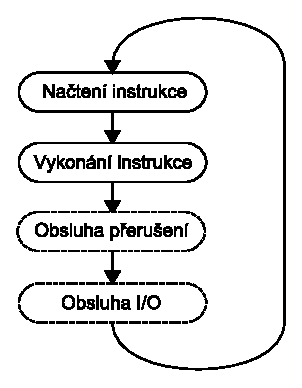
\includegraphics[width=4.5cm,height=6cm]{fig/anal_interpret}
\caption{Interpretační emulace\label{fig:anal_interpreter}}
\end{center}
\end{figure}

% Pamet

\subsection{Paměť}

Instrukce zpracovávané hlavním procesorem obvykle pracují s daty uloženými v
paměti, která je dalším významnou součástí emulovaného systému NEC PCEngine,
stejně jako mapovač, který procesoru umožňuje přistupovat k paměti v celém
rozsahu.

Emulovaná pamět je většinou realizována jako pre-alokované bloky paměti v rámci
platformy, na které emulátor běží. Tyto bloky jsou využívany v situaci, kdy
emulátor v emulovaném programu odchytí pokus o přístup do některého z regionů
paměti jako je RAM, ROM nebo vstupně-výstupní pamět namapovaná zařízeními.
Jednotlivé regiony paměti pak mají nastarost funkce emulující mapovač, které
zajišťují přepočet adresy a aplikaci případných restrikcí přístupu do paměti.

%TODO ukazka kodu?%

% Periferni zarizeni

\subsection{Periferní zařízení}

Systém NEC PCEngine je kromě samotného CPU HuC6280 vybaven řadou periferních
zařízení. Způsob emulace těchto zařízení je závislý na jejich účelu a druhu
činnosti.

Periferní zařízení jsou obvykle představována svým vnitřním stavem (obsah
interní paměti, registrů apod.) a případně uživatelským rozhraním. Často jsou
stejně jako procesor reprezentována datovou strukturou obsahující informace o
vnitřním stavu zařízení, nad kterou operují funkce volané emulačním kódem
procesoru. U zařízení, která disponují zmiňovaným uživatelským rozhraním, je
třeba funkčně zajistit propojení s uživatelským rozhraním emulátoru a patřičnou
konverzi vstupu/výstupu.

V případě systému NEC PCEngine je nutno brát v potaz zejména uživatelské
rozhraní následujících periferních zařízení:

\begin{itemize}
\item port herního ovladače
\item PSG
\item VDC HuC6270, VCE HuC6260
\end{itemize}

U řady zařízení je nutné si uvědomit, že prostředky použité k jejich emulaci
fungují diametrálně odlišně a proto nemusí být vždy nutné emulovat zařízení
zcela přesně. Např. systém vykreslování obrazu pomocí VDC HuC6270 a VCE HuC6260
na obrazovku je v případě emulátoru zcela odlišný (do bitové mapy) než u
původního hardware (na televizní obrazovku) a emulování videovýstupu až po
modulaci analogového signálu vhodného pro RF vstup televizního setu by bylo
zbytečné.

%TODO ukazka kodu?%

% Casovani

\subsection{Časování}

Ve skutečném hardware je časování a synchronizace jednotlivých komponent
zajišťena generátorem hodinových pulzů, který generuje pulzy o konstantní
frekvenci. Hodinový signál je pak vhodně předdělen a dodán jednotlivým
zařízením v systému. Z hlediska emulace existují dva základní přístupy k
časování s ohledem na:

\begin{description}
\item[přesnost] - kód emulátoru zpravidla odpočítává cykly procesoru během
	provádění emulovaného programu a jednotlivé zdroje časových pulzů jsou
	přímo emulovány pomocí služeb platformy, na které emulátor běží. To
	zaručuje dosažení věrohodné rychlosti emulace, pokud to dovolují prostředky
	této platformy. Tento přístup je vhodný spíše tam, kde je kladen důraz na
	průběh emulovaného programu a čas získání výsledku není kritický.

\item[rychlost] - původní zdroje hodinového signálu jsou zcela ignorovány a
	veškerá emulace probíhá maximální možnou rychlostí, kterou udává platforma,
	na které emulátor běží. Tento přístup se často používá při emulaci, kde je
	kladen důraz spíše na výsledek než průběh emulovaného programu.
\end{description}

V případě videoherních konzolí je rychlost provádění programu důležitým
faktorem. Většina herních programů je závislá na postřehu a zručnosti hráče a
rychlost provádění programu je častokrát přímo závislá na taktu procesoru,
protože narozdíl od různorodých konfigurací osobních počítačů je u videoherní
konzole tento parametr pro vývojáře konstantní. Provádění programu určeného pro
procesor s taktovací frekvencí 7.16MHz plnou rychlostí na procesoru s taktovací
frekvencí 2.0GHz bude, i přes výkonostní srážku způsobenou režií emulace, tak
rychlé, že bude program nepoužitelný.

Také je nutné vzít v úvahu fakt, že pro synchronizaci kódu a dění na obrazovce
se u videoherních systémů ve většině případů používá \uv{vertikální
synchronizace}. Do výpočtu časování tedy vstupuje další element - televizní
standard (NTSC nebo PAL), který přesně určuje počet řádků tvořících jeden
snímek, a kolikrát za vteřinu dojde k překreslení celého snímku.

% -----------------------------------------------------------------------------
% Pozadavky na program
% -----------------------------------------------------------------------------

\section{Požadavky na program}\label{chap:anal_requirements}

Úkolem výsledného programu je emulace videoherního systému NEC PCEngine v
rozsahu jeho základní verze, popsané specifikací uvedenou v
kapitole~\ref{chap:spec}, za použití výše popsaných technik a závěrů plynoucích
z rešerše existujících implementací v kapitole~\ref{chap:exist}.

%
% Funkcni pozadavky
%

\subsection{Funkční požadavky}

Výsledný program bude provádět následující činnosti:
\begin{itemize}
	\item načtení obrazu ROM pro NEC PCEngine \\
		\--- načte obraz ROM s programem ze souboru \\
		\--- provede potřebné úpravy obrazu ROM (rozdělení, ořez hlavičky)

	\item emulace zpracování programu \\
		\--- zpracuje interpretačním způsobem program v načteném obrazu ROM

	\item podpora emulace jednotlivých součástí NEC PCEngine \\
		\--- bude emulovat CPU HuC6280 a jeho interní periferní zařízení \\
		\--- bude emulovat základní funkce VDC HuC6270 a VCE HuC6260 \\
		\--- bude emulovat základní funkce PSG\footnote{PSG je fakticky
		součástí CPU HuC6280, ale jedná se o tak rozsáhlou a specifickou
		součást, že ji narozdíl od časovače nebo vstupně-výstupního paralelního
		portu uvádíme separátně.}

	\item interakce s uživatelem \\
		\--- vykreslí aktuální snímek generovaný VDC a VCE \\
		\--- přehraje zvuk generovaný PSG \\
		\--- zpracuje vstup z klávesnice jako vstup z herního ovladače
\end{itemize}

%
% Nefunkcni pozadavky
%

\subsection{Nefunkční požadavky}

Výsledný program bude mít následující vlastnosti:
\begin{itemize}
	\item přenositelnost kódu \\
		\--- bude možné ho sestavit a použít na platformách GNU/Linux a
			Microsoft Windows \\
		\--- bude možné ho jednoduše přenést na další platformy

	\item modularita \\
		\--- bude možné ho jednoduše rozšířit o další emulátory videoherních
			systémů \\
		\--- bude možné ho jednoduše rozšířit o další uživatelská
			rozhraní\footnote{Uživatelským rozhraním je zde myšlena vrstva
			využívající služeb platformy a zprostředkovávající vstup a výstup
			emulátoru uživateli.}

	\item implementační prostředí \\
		\--- bude napsán v jazyce C nebo C++
\end{itemize}

% -----------------------------------------------------------------------------
% Architektura programu
% -----------------------------------------------------------------------------

\section{Architektura programu}\label{chap:anal_architecture}

Architektura programu vychází z principů návrhu otevřeného software pro
operační systém UNIX popsaných v~\cite{Raymond04}. Její základní myšlenkou je
jednoduchost, rozšiřitelnost a oddělení jednotlivých logických částí programu.

Stěžejními prvky architektury programu jsou, přímo na základě nefunkčního
požadavku {\em modularity}, dva typy modulů:

\begin{itemize}
\item moduly emulátorů \\
	\--- zajišťují emulaci videoherních systémů
\item moduly uživatelských rozhraní \\
	\--- zajišťují rozhraní mezi emulátorem a uživatelem (obraz, zvuk, vstup)
\end{itemize}

Tyto moduly mají přesně specifikované rozhraní jak pro komunikaci mezi sebou,
tak pro komunikaci s jádrem programu, které zajišťuje inicializaci správné
dvojice modulů (vždy právě jednoho emulátoru a právě jednoho uživatelského
rozhraní) při spuštění a dále koordinuje jejich práci z hlavní programové
smyčky. Celkový pohled na architekturu programu je naznačen pomocí diagramu
analytického modelu tříd na obr.~\ref{fig:anal_arch}.

%TODO analyticky model
\begin{figure}[ht]
\begin{center}
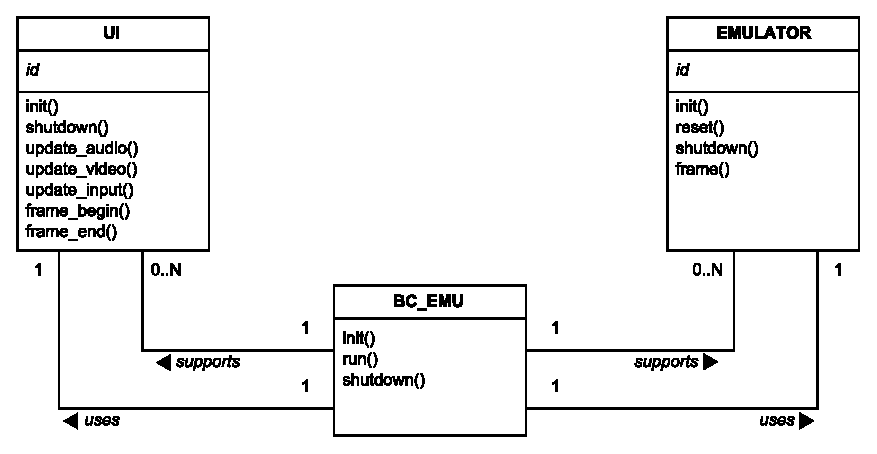
\includegraphics[width=14.2cm,height=7.1cm]{fig/anal_model}
\caption{Architektura programu\label{fig:anal_arch}}
\end{center}
\end{figure}

Kromě možnosti volby z více druhů emulátorů či uživatelských rozhraní, přinese
takto navržená architektura, podpořená možnostmi sestavovacího systému, také
možnost vytvořit personalizovaná sestavení obsahující jen moduly zvolené na
základě potřeb uživatele, nebo restrikcí plynoucích z možností platformy, pro
kterou bude výsledné sestavení programu určeno.

Modularita programu je tak navíc efektivním řešením nefunkčního požadavku na
{\em přenositelnost kódu}. Na platformách, kde nebude možné program sestavit z
důvodu např. závislosti na nedostupné knihovně uživatelského rozhraní, stačí
doimplementovat specifický modul založený na jiné, dostupné knihovně, který
bude \uv{suplovat} přenositelný kód. Poté stačí zavést příslušná omezení
sestavovacího systému pro nucený výběr takového modulu při sestavení pro tuto
platformu.

%
% Modul emulatoru
%

\subsection{Moduly emulátorů}

Emulátory jednotlivých videoherních systémů (v tomto případě NEC PCEngine)
jsou oddělenými moduly, komunikující s ostatními částmi programu pomocí
pevně specifikovaného rozhraní tvořeného několika funkcemi a datovými
strukturami pro výměnu dat. Analytická třída modulu emulátoru je naznačena
pomocí diagramu na obr.~\ref{fig:anal_emu}.

%TODO analyticky model s <<use>> na ty tri rozhrani
\begin{figure}[ht]
\begin{center}
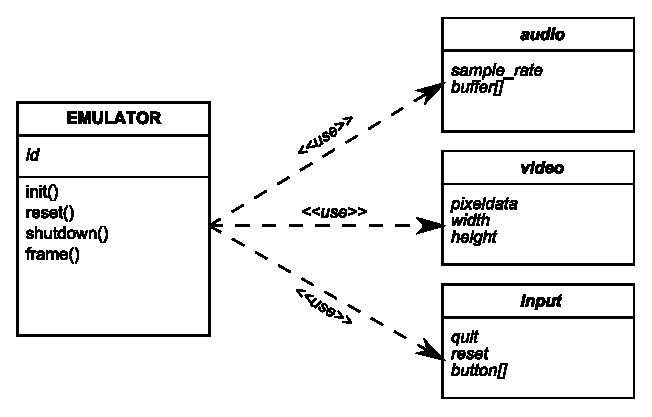
\includegraphics[width=10.5cm,height=6.4cm]{fig/anal_emu}
\caption{Analytická třída modulu emulátoru\label{fig:anal_emu}}
\end{center}
\end{figure}

Veřejné rozhraní modulu emulátoru tvoří, kromě struktur pro výměnu dat s
modulem uživatelského rozhraní (viz.
podsekce~\ref{chap:anal_architecture_struct}), následující funkce:
\begin{itemize}
\item {\it init()} - inicializace emulátoru (konstruktor)
\item {\it reset()} - re-inicializace emulátoru
\item {\it shutdown()} - ukončení činnosti emulátoru (destruktor)
\item {\it frame()} - posun v emulaci o jeden vykreslený snímek
\end{itemize}

Hlavní třídu modulu emulátoru je nutné chápat pouze jako zapouzdření funkčnosti
emulátoru. Je pochopitelné, že kód bude rozsáhlý a složitý a bude reflektovat
řadu specifik architektury konkrétního systému. Proto je architektura za
hranicí tohoto rozhraní zcela ponechána na autorovi konkrétního modulu.

Pro modul emulátoru systému NEC PCEngine je zvolena architektura tvořená čtyřmi
třídami, z nichž každá představuje jeden z funkčních bloků systému (CPU, VDC,
VCE a PSG), jehož vnitřní stav (registry, namapovaná paměť atd.) reprezentuje a
jehož chování emuluje pomocí svých metod.

%
% Moduly uzivatelskych rozhrani
%

\subsection{Moduly uživatelských rozhraní}

Úkolem modulu uživatelského rozhraní je zajistit interakci mezi uživatelem a
modulem emulátoru, resp. v něm běžícího programu. Zpravidla provádí následující
tři činnosti:

\begin{itemize}
\item zobrazit obrazová data získaná od modulu emulátoru
\item přehrát zvuková data získaná od modulu emulátoru
\item zpracovat uživatelský vstup a předat jej modulu emulátoru
\end{itemize}

Požadavek na {\em přenositelnost kódu} komplikuje potřeba programu používat
služby specifické pro určité platformy. Nepochybně největší částí programu
závislou na službách platformy je uživatelské rozhraní. I přes to, že existuje
řada knihoven a rámců zastřešujících práci s uživatelským rozhraním napříč více
platformami, nikdy se nepodaří jednou knihovnou či rámcem pokrýt všechny
možnosti. Oddělení kódu uživatelského rozhraní do modulu, jehož analytická
třída je naznačena pomocí diagramu na obr.~\ref{fig:anal_ui}, je tak logickým
krokem, který je v souladu i s použitím zmíněných knihoven a rámců\footnote{To
je ostatně i případ použité knihovny libSDL (viz. kapitola~\ref{chap:impl}),
díky které bude pro obě platformy dané požadavky, tedy GNU/Linux a Microsoft
Windows, zapotřebí pouze jeden modul uživatelského rozhraní.}.

\begin{figure}[ht]
\begin{center}
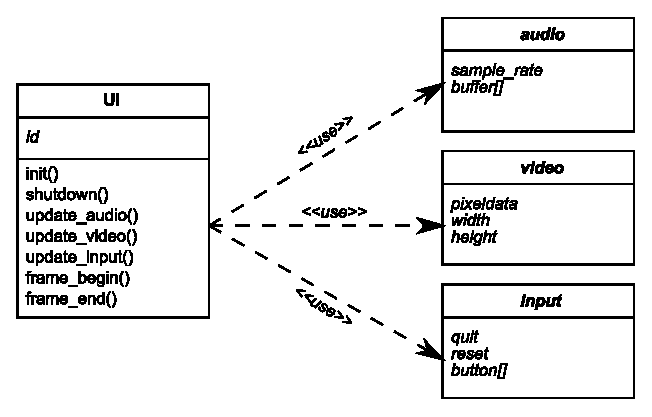
\includegraphics[width=10.5cm,height=6.4cm]{fig/anal_ui}
\caption{Analytická třída modulu uživatelského rozhraní\label{fig:anal_ui}}
\end{center}
\end{figure}

Tímto přístupem navíc docílíme možnosti snadné integrace s různými prostředími.
Modul uživatelského rozhraní nemusí být nutně interaktivní, jednou z mnoha
možností je např. síťová vrstva, která předává a přijímá informace od
vzdáleného klientu. Bez výraznějších úprav tak může výsledný program s tímto
modulem operovat v režimu klient/server po síti.

Moduly uživatelského rozhraní budou se zbytkem programu, podobně jako moduly
emulátorů, komunikovat pomocí pevně specifikovaného rozhraní, které bude
tvořeno, kromě struktur pro výměnu dat s modulem emulátoru (viz.
podsekce~\ref{chap:anal_architecture_struct}), následujícími funkcemi:

\begin{itemize}
\item {\it init()} - inicializace uživatelského rozhraní (konstruktor)
\item {\it shutdown()} - ukončení činnosti uživatelského rozhraní (destruktor)
\item {\it update\_audio()} - aktualizace zvukového výstupu
\item {\it update\_video()} - aktualizace obrazového výstupu
\item {\it update\_input()} - aktualizace vstupu
\item {\it frame\_begin()} - činnost před vykreslením snímku
\item {\it frame\_end()} - činnost po vykreslení snímku
\end{itemize}

Modul uživatelskéh rozhraní obsahuje synchronizační mechanismus tvořený dvojicí
funkcí {\it frame\_begin()} a {\it frame\_end()}. Ten umožňuje provádět kód
před zahájením vykreslení snímku a po jeho ukončení.

Protože mají knihovny a rámce použité pro práci s uživatelským rozhraním
většinou přímý přístup k platformně závislým službám, jako je např. správa
časovačů, je logické umístit mechanismus pro časovou synchronizaci pomocí
těchto služeb právě do modulu uživatelského rozhraní. Kód vykonávaný touto
dvojicí funkcí může např. měřit délku snímku a kompenzovat počet snímků za
sekundu.

%
% Spolecne struktury pro vymenu dat
%

\subsection{Společné struktury pro výměnu
dat}\label{chap:anal_architecture_struct}

Rozhraní obou typů modulů dotváří trojice pomocných struktur určených k výměně
dat v pevně daném formátu. To zajišťuje, že si libovolná, správně provedená
implementace modulu emulátoru \uv{bude rozumět} s libovolnou, správně
provedenou implementací modulu uživatelského rozhraní a naopak. Jedná se o
následující struktury:

\begin{itemize}
\item {\it audio} - pro výměnu informací o zvukovém výstupu (emulátor
	$\rightarrow$ uživatelské rozhraní)
\item {\it video} - pro výměnu informací o obrazovém výstupu (emulátor
	$\rightarrow$ uživatelské rozhraní)
\item {\it input} - pro výměnu informací o stavu vstupu (uživatelské rozhraní
	$\rightarrow$ emulátor)
\end{itemize}

%%%%%%%%%%%%%%%%%%%%%%%%%%%%%%%%%%%%%%%%%%%%%%%%%%%%%%%%%%%%%%%%%%%%%%%%%%%%%%%
% bc.tex - Bachelor thesis                                                    %
% Subject: bc_emu - portable video game emulator                              %
% Chapter: Implementace                                                       %
% Author: Ondrej Balaz <ondra@blami.net>                                      %
%%%%%%%%%%%%%%%%%%%%%%%%%%%%%%%%%%%%%%%%%%%%%%%%%%%%%%%%%%%%%%%%%%%%%%%%%%%%%%%

\chapter{Implementace}\label{chap:impl}

Implementace spočívá v převodu navržené architektury do podoby spustitelného
kódu. Způsob jakým jsou jednotlivé části programu implementovány je dán volbou
programovacího jazyka a knihoven popsanou v sekci~\ref{chap:impl_env} této
kapitoly, ale také použitím specifických implementačních technik a konvencí
popsaných v sekci~\ref{chap:impl_techniques}.

Následující sekce kapitoly rámcově rozebírají základní myšlenky použité při
implementaci programového jádra (sekce~\ref{chap:impl_program}), modulu
emulátoru systému NEC PCEngine (sekce~\ref{chap:impl_pce}) a modulů
uživatelských rozhraní libSDL (sekce~\ref{chap:impl_sdl}) a libSDL s podporou
OpenGL (sekce~\ref{chap:impl_sdlgl}).

K podrobnějšímu studiu implementace poslouží zdrojový kód programu, který je
okomentován a psán tak, aby byl co nejvíce čitelný. Tam kde je to vhodné jsou v
kódu (hlavně emulátoru systému NEC PCEngine) uvedeny i části specifikace.
Veškeré komentáře v kódu jsou zpracovatelné systémem Doxygen~\cite{wwwDoxygen}
do přehledné programátorské dokumentace.

Kapitolu uzavírá sekce~\ref{chap:impl_cmake}, která se věnuje použití
sestavovacího systému CMake za účelem konfigurace sestavení a sestavení
programu.

% -----------------------------------------------------------------------------
% Implementacni prostredi
% -----------------------------------------------------------------------------

\section{Implementační prostředí}\label{chap:impl_env}

Implementace emulátoru je nelehký úkol, který vyžaduje, kromě znalosti
architektury emulovaného systému a jeho asembleru, také dobrou znalost
programovacího jazyka, ve kterém bude implementace probíhat. Nejvhodnějšími
kandidáty z kategorie vyšších programovacích jazyků jsou jazyky C a C++, které
disponují datovým typem ukazatel a dovolují přímou práci s pamětí. Zároveň se
jedná o nejrozšířenější jazyky kompilované do nativního kódu cílové platformy.

%
% Programovaci jazyk
%

\subsection{Programovací jazyk}\label{chap:impl_env_lang}

Pro implementaci programu byl z nabízené dvojice programovacích jazyků C a C++
zvolen programovací jazyk C. Toto rozhodnutí je založeno na mých zkušenostech s
touto dvojící programovacích jazyků, ze kterých ovládám více právě programovací
jazyk C.

Ačkoliv je architektura programu navržena částečně objektově, zdaleka nenachází
plné využití možností objektového programování (rozsáhlé abstrakce, složitá
hierarchie tříd vyžadující komplexní využití dědičnosti atd.). Možnosti, které
z tohoto přístupu k programování využívá lze bez větších problémů implementovat
i v jazyce C při dodržení určitých postupů a konvencí, o kterých podrobně
pojednává např.~\cite{Schreiner94}.

Programovací jazyk C má navíc několik vlastností, které ulehčí přenositelnost
výsledného řešení na případné méně standardní platformy. Jedná se o:

\begin{itemize}
\item jazyk C má oproti jazyku C++ méně běhových závislostí, což ho favorizuje
	v případě programování nízkoúrovňových systémů, vestavěných zařízení apod.,
	na která by program mohl být v budoucnu přenášen.

\item jazyk C neprovádí transformaci jmen symbolů, což je velice užitečné při
	např. při lazení a optimalizacích na úrovni assemblerového kódu programu.

\item jazyk C umožňuje, narozdíl od jazyka C++ uložení polí proměnné délky na
	zásobník, kde je alokace velice rychlá. Na některých platformách by toto
	mohlo posloužit k uložení kritických míst emulované paměti.
\end{itemize}

%
% Knihovny a nastroje
%

\subsection{Knihovny a nástroje}\label{chap:impl_env_tools}

K implementaci uživatelského rozhraní je, po vzoru emulátoru Mednafen uvedeného
v rešerši existujících řešení (viz. kapitola~\ref{chap:exist}), použita
knihovna pro tvorbu uživatelských rozhraní libSDL~\cite{wwwlibSDL} a knihovna
pro akcelerovanou grafiku OpenGL~\cite{wwwOpenGL}. Kód používající tyto
knihovny je zapouzdřen do modulu uživatelského rozhraní, nikoliv použit přímo,
a tak může být kdykoliv nahrazen.

Důvodem použití právě těchto knihoven je fakt, že podporují obě, nefunkčními
požadavky, vytyčené platformy (tj. GNU/Linux a Microsoft Windows). Nebude tedy
nutné vytvářet speciální modul uživatelského rozhraní pro každou z těchto
platforem.

Pro konfiguraci sestavení a programu se využívá multiplatformního sestavovacího
nástroje CMake~\cite{wwwCMake}. Více o použití tohoto nástroje je uvedeno v
sekci~\ref{chap:impl_cmake} této kapitoly.

Součástí implementačního prostředí jsou nepochybně i nástroje využité k psaní a
lazení testovacích programů pro procesor HuC6280 - tedy emulátor procesoru 6502
- M6502~\cite{wwwM6502} a assembler pro procesor HuC6280 -
MagicKit~\cite{wwwMagicKit}.

% -----------------------------------------------------------------------------
% Techniky pouzite pri implementaci
% -----------------------------------------------------------------------------

\section{Techniky použité při implementaci}\label{chap:impl_techniques}

Na základě některých nefunkčních požadavků a použití zvolených nástrojů byly
při implementaci použity techniky popsané v následujícím textu.

%
% Objektový přístup a zapouzdření
%

\subsection{Objektový přístup a zapouzdření}\label{chap:impl_techniques_obj}

Objektově orientovaná analýza a návrh software jsou postupy založené na
modelování skutečné reality v programu pomocí tzv. \uv{objektů}. Tyto objekty
jsou zpravidla tvořeny atributy reprezentujícími stav objektu a metodami,
pomocí kterých mohou tento stav ovlivňovat ostatní objekty v modelu. Více o
objektově orientovaném programovacím stylu lze nalézt např v.~\cite{Booch94}.

Analýza a návrh programu byly přirozeně provedeny touto cestou a jednotlivé
jeho části jsou tvořeny objekty, které zapouzdřují činnost těchto částí.

Pro implementaci byl zvolen programovací jazyk C, který, jak už bylo uvedeno,
nemá přímou podporu metodik objektového programování. Nicméně objektově
orientovaná architektura progamu je poměrně jednoduchá a nestaví žádné
závážnější překážky implementaci v tomto jazyce. Pro potřeby implementace
navržené architektury si vystačíme s následujícími technikami:

\begin{description}
\item[třída] - je implementována pomocí datové struktury sdružující všechny
	atributy objektů této třídy a množiny funkcí, které představují
	metody této třídy.

\item[instance] - instance je tvořena ukazatelem na dříve popsanou strukturu
	třídy, které odpovídá. Vytvoření instance proběhne alokací paměti (pomocí
	funkce jazyka C {\em malloc()}) pro tuto strukturu a případně zavoláním
	funkce, která zinicializuje její prvky (konstruktoru). Zrušení instance pak
	proběhne jednoduše uvolněním paměti pro strukturu (pomocí funkce jazyka C
	{\em free()}), případně jemu předcházejícím zavoláním funkce, která provede
	např. uložení dat ze struktury na disk před jejím zánikem (destruktoru).

\item[metoda] - je funkce, jejímž prvním argumentem je vždy ukazatel na konkrétní
	instanci objektu. Tato funkce při svém volání ověří existenci (např. pomocí
	makra jazyka C {\em assert()}) a vykoná činnost.

\item[atribut] - je členská proměnná struktury třídy. Pokud se jedná o ukazatel
	do paměti, měl by destruktor třídy zajistit uvolnění této paměti, pokud je
	to žádoucí.
\end{description}

% TODO priklad kodu tridy? %

Protože návrh programu nepočítá s tím, že by od některé třídy mělo existovat
více instancí, jsou v rámci zdrojového kódu programu instance globální a
nepředávají se metodám. Tento přístup může do budoucna znamenat nepřehlednost
kódu a proto je považován za chybu, která bude odstraněna.

%
% Prenositelnost kodu
%

\subsection{Přenositelnost kódu}

Dalším aspektem úzce spojeným s volbou jazyka C je přenositelnost kódu. Protože
se zdrojový kód programů napsaných v jazyce C překládá přímo do strojového
kódu, není možné přenášet výsledné binární soubory mezi platformami. Místo toho
je nutné pro každou z podporovaných platforem kód přeložit pro ni určeným
překladačem jazyka C.

Kromě toho, že je nutné architektonicky oddělit kód závislý na platformě tak,
jak je to popsáno v kapitole~\ref{chap:anal}, je také nutné vzít v potaz
několik dalších faktorů, které ovlivňují přenositelnost kódu.

% Standardy jazyka C

\subsubsection{Standardy jazyka C}

I přesto, že je množina základních datových typů, knihovních funkcí apod. v
jazyce C předepsaná standardem ANSI C, řada distribucí vývojových nástrojů
jazyka C se liší v jeho výkladu, zavádí jiné pojmenování pro datové typy,
nebo nedefinuje některá makra.

Z toho důvodu existuje soubor {\tt xtypes.h}, kde jsou definovány jednotlivé
datové typy, které by měly být používany v přenositelném kódu. V případě, že
nastane potřeba pro specifický překladač nebo platformu definovat typ jinak,
bude možné to provést podmíněně na jednom místě.

V některých případech navíc není možné, aby překladač odpovídal
standardu\footnote{Např. v případě vývojového prostředí devkitPro pro Nintendo
DS je nutné aby program místo standardní vstupní funkce {\em main()} obsahoval
dvě vstupní funkce z nichž každá je určena pro jeden z dvojice v systému
přítomných procesorů.}. Pro tento případ je i jádro programu rozděleno na dvě
části z nichž jedna implementuje na platformě nezávislý kód a druhá kód na
platformě závislý.

% Endianita

\subsubsection{Endianita}

Endianita (pořadí bajtů) architektury, na které emulátor běží, má v případě
implementace v jazyce C významný dopad na jeho funkčnost. Jak již bylo uvedeno
v kapitole~\ref{chap:anal}, paměť emulovaného systému je reprezentována přímo
pre-alokovanými bloky paměti, uspořádánými dle endianity této architektury.
Emulovaný program ale pracuje s uspořádáním paměti daným endianitou emulovaného
procesoru. V případě že se tyto endianity liší, je nutné na kritických místech
pořadí bajtů obrátit.

Aby těchto míst v kódu programu vznikalo co nejméně, je v souboru {\tt
xtypes.h} zaveden speciální union {\em pair} představující dvojici slov,
jehož definice je následující:

\begin{verbatim}
typedef union {
#ifdef LSB
    struct { uint8 l,h,h2,h3; } b;
    struct { uint16 l,h; } w;
#else
    struct { uint8 h3,h2,h,l; } b;
    struct { uint16 h,l; } w;
#endif
    uint32 d;
} pair;
\end{verbatim}

Pro přístup k celé dvojici slov reprezentované tímto unionem lze použít jeho
prvek {\em d}, pro přístup k hornímu slovu pak prvek {\em w.h} atd. Interní
struktura tohoto unionu je stanovena v okamžiku sestavování programu nastavením
makra {\em LSB}, resp. {\em MSB}, tak aby bylo v kódu přistupováno k žádanému
slovu nebo bajtu.

Jedno z dvojice maker {\em LSB}, {\em MSB}, je vždy nastaveno sestavovacím
systémem CMake na základě informace o endianitě architektury, pro kterou
probíhá sestavení. Podobně jako je použito v případě unionu {\em pair} ho lze
použít na libovolném místě v kódu, kde je nutné zařídit aby data byla správně
reprezentována emulovanému programu a nelze tam union {\em pair} použít (např.
kód VDC nebo PSG).

%
% Konvence dodrzovane v kodu
%

\subsection{Konvence dodržované v kódu}

V kódu jsou pro lepší přehlednost a srozumitelnost dodržovány následující
konvence:

\begin{itemize}
\item názvy identifikátorů jsou tvořeny malými písmeny a podtržítky
\item konstruktory tříd jsou nazvány {\em init}
\item destruktory tříd jsou nazvány {\em shutdown}
\item názvy metod jsou prefixovány názvem příslušné třídy
\item identifikátory v rámci modulu jsou prefixovány názvem modulu
\end{itemize}

% -----------------------------------------------------------------------------
% Program
% -----------------------------------------------------------------------------

\section{Program}\label{chap:impl_program}

Celý program je příznačně nazván {\em bc\_emu}. Skládá se z programového jádra,
platformně závislého kódu pro spuštění z příkazové řádky operačního systému
osobního počítače a následující trojice modulů:

\begin{itemize}
\item emulátoru systému NEC PCEngine ({\em pce})
\item uživatelského rozhraní libSDL ({\em sdl})
\item uživatelského rozhraní libSDL s podporou OpenGL ({\em sdlgl})
\end{itemize}

\subsection{Podpora modulů}

Podpora modulů v programu je implementována pomocí ukazatelů na
funkce~\cite{wwwCFuncPointer}. Při konfiguraci sestavení je systémem CMake
vygenerován soubor {\tt bc\_emu\_modules.c}, který obsahuje dvojici polí
struktur modulů (emulátorů a uživatelských rozhraní) obsahujících ukazatele na
funkce, které tvoří veřejné rozhraní jednotlivých modulů.

Po sestavení má program tyto dvě pole k dispozici a při spuštění jen provede
nastavení globálních ukazatelů podle aktuálně zvolené dvojice modulů. Obecné
rozhraní je dotvořeno trojicí globálních společných datových struktur pro
výměnu dat mezi moduly, definovaných v souboru {\tt interface.h}.

Tento způsob je plně vyhovující pokud budeme předpokládat
statické\footnote{Knihovny jednotlivých modulů jsou přímo připojeny do
binárního souboru programu.} sestavování výsledného programu a fakt, že nikdy
nebude zapotřebí více instancí jednoho typu modulu. Při běžném používaní
programu zamýšleným způsobem budou tyto předpoklady vždy splněny. Pokud by
nastal důvod sestavit program dynamicky\footnote{Knihovny jednotlivých modulů
jsou načítány službou operačního systému při každém spuštění programu.}, bylo by
nutné vhodně rozšířit funkce pro hledání jednotlivých typů modulů v souboru
{\tt module.c}. Podpora více instancí modulu bude vyřešena opravením chyby s
předáváním ukazatele na instanci popsané v
podsekci~\ref{chap:impl_techniques_obj}.

% -----------------------------------------------------------------------------
% Modul emulatoru NEC PCEngine
% -----------------------------------------------------------------------------

\section{Modul emulátoru NEC PCEngine}\label{chap:impl_pce}

Modul emulátoru systému NEC PCEngine je nejvýznamnější částí programu. Obsahuje
veškerý kód zajišťující emulaci jednotlivých částí tohoto systému. Soubory se
zdrojovými kódy modulu jsou umístěny v adresáři {\tt /emu/pce/}.

Nejpodstatnější funkcí celého modulu je bezpochyby funkce {\it pce\_frame()},
která zajišťuje posun o vykreslení jednoho obrazového snímku v emulovaném
programu. Standard NTSC má při kmitočtu 60Hz 59.9 prokládaných snímků tvořených
263-mi řádky.

%
% CPU
%

\subsection{CPU HuC6280}

Veškerá emulace činnosti CPU HuC6280 je zapouzdřena do třídy {\em pce\_cpu}.
Základ této třídy tvoří soubor {\tt cpu\_huc6280.c}, který obsahuje řadu metod
pro samotnou práci s procesorem a soubory instrukční sady: {\tt
cpu\_instr.inc}, {\tt cpu\_instr\_util.inc} a {\tt cpu\_op\_tab.inc}.
Implementace částečně vychází z emulátoru procesoru M6502 Juergena
Buchmuellera.

% Casovani

\subsubsection{Časování}\label{chap:impl_pce_cpu_timing}

Emulátor systému NEC PCEngine je naimplementován tak, aby počet procesorových
cyklů prováděných při vykreslení jednoho řádku snímku odpovídal skutečnému
hardware. Tento počet cyklů lze získat následujícím výpočtem:

$$ n_{cykly} = \frac{f_{VDC}}{n_{snimky} * n_{radky}} = 
	\frac{7,16 * 10^6}{59.9 * 263} \approx 455 $$

kde $f_{VDC}$ je taktovací frekvence VDC~\cite{Schleussinger98}, $n_{snimky}$
je počet prokládaných snímků za sekundu dle standardu NTSC a $n_{radky}$ je
počet řádků tvořících jeden proložený snímek (čitatel je počet vykreslených
řádků za sekundu).

Vzhledem k tomu, že dochází k vykonání přesného počtu procesorových cyklů během
vykreslení řádku a tedy i snímku, bude při počtu snímků za sekundu definovaném
standardem NTSC rychlost emulace věrohodná. To je stav, který je z hlediska
modulu emulátoru vyhovující.

Nicméně pokud není v hlavní programové smyčce, ze které vykreslování
jednotlivých snímků probíhá (soubor {\tt bc\_emu.c}), provedeno omezení počtu
vykreslených snímků na přibližně tuto hodnotu, bude rychlost emulace omezená
pouze rychlostí platformy na které emulátor běží, tedy pravděpodobně příliš
vysoká.

Odstranění této chyby, která není v kódu emulátoru a nelze jí řešit bez použití
služeb knihovny nebo rámce uživatelského rozhraní, případně platformy, je
přenecháno dvojici funkcí {\em frame\_begin()} a {\em frame\_end()} modulu
uživatelského rozhraní (viz.~\ref{chap:impl_sdl_timing}).

% Zpracovani instrukci

\subsubsection{Zpracování instrukcí}

Stěžejní částí emulace CPU HuC6280 je zpracování instrukcí, které probíhá v
rámci metody {\it pce\_cpu\_exec()}. Jejím argumentem je počet procesorových
cyklů k dispozici (pro jeden snímek 455) a návratovou hodnotou je buď záporné
číslo vyjadřující počet chybějících cyklů (instrukce se vykonávají atomicky,
takže byly cykly provedeny navíc), nebo kladné číslo vyjadřující počet cyklů,
který přebyl.

Jednotlivé instrukce jsou implementovány jako inline\footnote{Označení pro
funkce, které překladač jazyka C překládá tak, že v místě volání funkce nevloží
do strojového kódu odskok na rutinu představující kód funkce, ale přímo tento
kód} funkce uspořádané do pole, kde indexem je přímo opkód. Definice těchto
funkcí lze nalézt v přehledné tabulce v souboru {\tt cpu\_op\_tab.inc} a mají
typicky tvar:

\begin{verbatim}
OP(016) { int arg1; cycl_n -= 6;    RD_ZPX;         ASL;        WB_EAZ; }
\end{verbatim}

Kromě deklarace proměnných představujících operandy instrukce a dekrementace
počtu zbývajících cyklů procesoru, tvoří tělo každé funkce implementující
instrukci jedno až tři makra.

Makra s dvoupísmenným prefixem (např. {\tt RD\_ZPX} nebo {\tt WB\_EAZ})
zajišťují přístup do paměti s použitím konkrétního adresního módu. Zdrojový kód
těchto maker je umístěn v souboru {\tt cpu\_instr\_util.inc} a jejich úkolem je
spočítat adresu a obsah paměti na této adrese načíst do připravené proměnné
jako operand instrukce, případně obsah této proměnné nebo některého z registrů
na tuto adresu uložit.

Zbývající makro pak zajišťuje samotnou emulaci instrukce. Zdrojový kód
jednotlivých maker instrukcí je umístěn v souboru {\tt cpu\_instr.inc}.

Z předchozího popisu je zřejmé, že při implementaci cyklického zpracování
instrukcí tímto způsobem stačí v interpretační funkci inkrementovat čítač
programu ({\sf PC}) a zavolat funkci z pole s indexem jeho nové hodnoty.

% Zpracovani preruseni

\subsubsection{Zpracování přerušení}

Implementace emulace CPU HuC6280 bere v potaz zpracování přerušení na všech
linkách přerušení. V případě, že během emulace programu nastane přerušení, je
na příslušné lince nastaven mód \uv{aserce}. Po zpracování přerušení je linka
uvedena zpět do módu \uv{volno}. Stav jednotlivých linek přerušení je uchován
pomocí pole {\it irq\_state[]} v rámci struktury třídy {\it pce\_cpu}.

Zpracování přerušení je implementováno pomocí makra {\it CHECK\_IRQ\_LINES},
které kontroluje stav jednotlivých linek a v případě, že je některá z nich
nastavena na stav \uv{aserce}, zavolá další makro {\it DO\_INTERRUPT} s
vektorem příslušného přerušení v argumentu. Zdrojový kód obou maker je
umístěn v souboru {\tt cpu\_instr\_util.inc}.

Kromě běžného ošetření v rámci emulovaného programu (odskok na vektor přerušení
a spuštění ošetřující rutiny) je navíc volána funkce zpětného volání, na níž
byl nastaven ukazatel pomocí funkce {\it pce\_cpu\_set\_irq\_callback()}. Tato
funkce dostává parametrem identifikátor linky, na které došlo k přerušení.
Tento mechanismus je výhodný např. pro lazení.

%
% VDC + VCE
%

\subsection{VDC HuC6270 + VCE HuC6260}

Emulace zobrazovacího subsystému NEC PCEngine je zajištěna třídami {\it
pce\_vdc} a {\it pce\_vce}. Jejich kód nalezneme v souborech {\tt
vdc\_huc6270.c} a {\tt vce\_huc6260.c}. Výstup obrazových dat je proveden
jejich vykreslením do bitové mapy reprezentované strukturou {\it t\_video},
kterou dále zpracovává modul uživatelského rozhraní.

Vzhledem k tomu, že předmětem práce nebylo studium způsobu zobrazování na
televizoru, emulace VDC i VCE postrádá implementaci řady vlastností (barva
překryvu v prostoru nevyužité obrazovky, nastavení šířky bodových pulzů atd.),
které nijak výrazně neovlivňují funkčnost modulu emulátoru a mohou být doplněny
později.

% VDC

\subsubsection{VDC HuC6270}

Třída {\it pce\_vdc} zajišťuje veškeré vykreslovací operace. Vykreslování
výsledného obrazu do bitové mapy je, stejně jako vykreslování na obrazovku
televizoru v případě skutečného hardware, prováděno po jednotlivých řádcích.
Tento přístup zvyšuje přesnost emulace u programů, které využívají k
synchronizaci přerušení vyvolaných před samotnou {\em vertikální synchronizací}
(např. raster compare, nebo kolize sprajtu 0).

Ústřední funkcí třídy {\it pce\_vdc} je {\it pce\_vdc\_render\_line()}, jejímž
argumentem je číslo právě vykreslovaného řádku. Podle jednotlivých povolených
rovin deleguje tato funkce činnost vykreslování řádku na funkce {\it
pce\_vdc\_render\_bp()}, která provádí vykreslování dlaždic pozadí, a
{\it pce\_vdc\_render\_sp()}, která provádí vykreslování sprajtů. Obě tyto
funkce pracují s emulovanými atributovými tabulkami {\em BAT} a {\em SAT}. V
případě sprajtů, jejichž vykreslování je ovlivněno řadou atributů v tabulce
{\em SAT} jsou jednotlivé záznamy reprezentovány strukturou {\it
t\_pce\_vdc\_sprite}.

Pro urychlení a zpřehlednění vykreslovacího kódu se namísto vykreslování vzorů
dlaždic pozadí a sprajtů přímo z videopaměti používá dvojice vyrovnávacích
pamětí, kde jsou jednotlivé vzory předvykresleny a uloženy. Aby nedocházelo ke
zbytečnému přegenerovávání obsahu obou vyrovnávacích pamětí při každém
vykreslování, jsou záznamy \uv{znečišťovány} při přístupu do odpovídající části
videopaměti a regenerační algoritmus obnovuje jen tyto \uv{znečištěné} záznamy.
Regerenerace obou vyrovnávacích pamětí je zajištěna funkcemi {\it
pce\_vdc\_cache\_bp()} a {\it pce\_vdc\_cache\_sp()}.

% VCE

\subsubsection{VCE HuC6260}

Třída {\it pce\_vce} zajišťuje správu barevných informací při vykreslování
výsledného obrazu třídou {\it pce\_vdc}.

Kromě emulace jednotlivých registrů skutečného VCE třída spravuje dvě
vyhledávací tabulky {\it pixel\_lut} a {\it bp\_lut}. První z těchto tabulek
umožňuje dohledávat složkově definovanou barevnou informaci (potřebnou k
vykreslení pixelu do bitové mapy) pomocí indexu barvy VCE, a druhá pak slouží k
dohledání správné bitové roviny podle indexu barvy v planárním způsobu uložení
obrazových dat.

Formát pixelu\footnote{Formát pixelu udává které bity v rámci reprezentace
pixelu vyjadřují kterou barevnou složku.} v tabulce {\it pixel\_lut} je v
současné době pevně dán tak, aby se shodoval s tím, který používá knihovna
libSDL. Z hlediska použití růzých knihoven pro uživatelské rozhraní by bylo
výhodnější umožnit nastavení formátu pixelu v rámci třídy {\it vce} na takový,
který použitá knihovna očekává. Vzhledem k současné implementaci může na
platformách, sice podporovaných knihovnou libSDL, ale s jiným formátem pixelu,
dojít k barevné deformaci výstupního obrazu.

%
% PSG
%

\subsection{PSG}

Vzhledem k možnostem PSG systému NEC PCEngine je emulace zvukového výstupu
poměrně složitý problém. Základní implementace v souboru {\tt psg.c}
nezohledňuje řadu možností které PSG nabízí.

Emulace zvukového výstupu je implementována funkcí {\it pce\_psg\_fill()},
jejímž úkolem je naplnit vyrovnávací paměť pro jednotlivé zvukové kanály daty,
která vzniknou na základě smíšení emulovaných kanálů PSG. To je provedeno tak,
že pro každý sampl výsledného zvukového jsou iterativně zpracovány všechny
emulované kanály PSG v příslušném samplu. Takto naplněná vyrovnávací pamět je
předána v rámci struktury {\it t\_audio} modulu uživatelského rozhraní.

Současná implementace PSG nepodporuje přímý přístup k datům (režim DDA) a
přespříliš neřeší synchronizaci a časování zvuku. Vyrovnávací paměť zvukového
výstupu je plněna vždy po vykreslení snímku (při vertikální synchronizaci),
což odpovídá způsobu zpracování zvuku většinou herních programů.

Formát výstupního zvuku\footnote{Formát je u digitálního zvuku tvořen zpravidla
délkou jednotlivých samplů, pořadím bajtů, frekvencí a přesností a znaménkem
čísla reprezentujícího sampl.} je opět pevně nastaven na stejný, jaký používá
knihovna libSDL a z hlediska použití jiných knihoven by měla třída {\it
psg} umožňovat jeho nastavení v souladu s očekáváním použité knihovny.

%
% Parser obrazu ROM
%

\subsection{Parser obrazů ROM}

Implementace přenositelného parseru obrazů ROM je provedena tak, že namísto
práce se souborem, se pracuje s ukazatelem na oblast paměti, kde jsou ve
struktuře uložena data, o kterých se celý program domnívá, že jsou obrazem
paměti ROM. Jak se taková data do příslušné struktury dostanou je pak problém,
který řeší jádro. Toto řešení bere v potaz situaci, kdy by program mohl být
portován na architekturu, kde neexistuje souborový systém a data uložená v ROM
jsou reprezentována např. pouze ukazatelem do paměti.

Samotný parser obrazů ROM přečte během inicializace modulu emulátoru obsah ROM
a na základě velikosti předané ve struktuře {\it t\_rom} společně s daty
provede analýzu a nutné kroky jako je oddělení hlavičky nebo rozdělení obrazu.
Tyto kroky jsou popsány v kap.~\ref{chap:spec}.

% -----------------------------------------------------------------------------
% Modul uzivatelskeho rozhrani libSDL
% -----------------------------------------------------------------------------

\section{Modul uživatelského rozhraní libSDL}\label{chap:impl_sdl}

Modul uživatelského rozhraní libSDL umožňuje uživatelskou interakci s modulem
emulátoru. Zpracovává uživatelský vstup, poskytuje obrazový a zvukový výstup a
zajišťuje omezení počtu vykreslených snímků. Na jeho vývoj nebyl kladen
přílišný důraz, protože se jedná o modul implementující pouze základní
funkčnost uživatelského rozhraní pro potřeby demonstrace výsledků dosažených
při implementaci modulu emulátoru NEC PCEngine. Soubory se zdrojovými kódy
tohoto modulu se nacházejí v adresáři {\tt /ui/sdl}.

Tento modul je tvořen jedinnou třídou {\em pce\_sdl}, která obsahuje funkce pro
zpracování dat ve strukturách {\it t\_audio}, {\it t\_video} a {\it t\_input} a
dvojici funkcí {\it sdl\_frame\_begin()} a {\it sdl\_frame\_end()} pro vykonání
kódu před a po vykreslení každého snímku modulem emulátoru.

\subsection{Omezení počtu vykreslených snímků}\label{chap:impl_sdl_timing}

Jak již bylo uvedeno dříve (viz.~\ref{chap:impl_pce_cpu_timing}), modul
emulátoru systému NEC PCEngine je naimplementován tak, aby dosahoval věrohodné
rychlosti při vykreslení cca. 60-ti snímků během jedné sekundy (což přibližně
odpovídá počtu proložených snímků za sekundu dle standardu NTSC).

Omezení počtu vykreslených snímků je provedeno pomocí dvojice atributů v rámci
třídy {\em sdl}. Tím prvním je počet \uv{tiků} před zahájením vykreslování
snímku {\em ticks\_odl}, tím druhým pak počet \uv{tiků} po dokončení
vykreslování. Tyto hodnoty jsou nastaveny funkcemi {\it sdl\_frame\_begin()} a
{\it sdl\_frame\_end()} při každém vykreslování snímku. Při volání funkce
poslední zmíněné funkce jsou zároveň tyto hodnoty odečteny a pokud v rámci
vykresleného snímku zbývá čas do $\frac{1}{60}~sekundy$, jednoduše se o tento
čas prodlí vykreslení následujícího snímku.

\subsection{Interakce s uživatelem}

Propojení a způsob práce se vstupními a výstupními zařízeními je provedeno
pevně ve zdrojovém kódu programu a uživatel nemá možnost ho modifikovat. V
současné implementaci je výstupní rozlišení programu 640x480 pixelů v barevné
hloubce 16 bitů, což je nastavení pokrývající potřeby většiny herních programů.
Obraz není deformován na velikost okna, ale vykreslován od pravého horního rohu
do velikosti určené aktuálním rozlišením VDC. Tlačítka herního ovladače a
ovládaní běhu programu jsou mapována na tlačítka klávesnice podle
tabulky~\ref{tab:sdl_keymap}.

\begin{table}[ht]
\begin{center}
\begin{tabular}{|l|l|}
\hline
\textbf{Klávesa} & \textbf{Význam} \\
\hline
{\tt <nahoru>} & směrový kříž herního ovladače, směr nahoru \\
{\tt <dolů>} & směrový kříž herního ovladače, směr dolů \\
{\tt <vlevo>} & směrový kříž herního ovladače, směr vlevo \\
{\tt <vpravo>} & směrový kříž herního ovladače, směr vpravo \\
{\tt <enter>} & tlačítko \uv{Start} herního ovladače \\
{\tt a} & tlačítko \uv{I.} herního ovladače \\
{\tt s} & tlačítko \uv{II.} herního ovladače \\
\hline
{\tt r} & restart emulace \\
{\tt q} & ukončení programu \\
\hline
\end{tabular}
\end{center}
\caption{Mapování kláves v modulu uživatelského rozhraní
libSDL\label{tab:sdl_keymap}}
\end{table}

Na obr.~\ref{fig:impl_sdl} je zobrazena sejmutá obrazovka s výstupem emulace
herního programu {\em Skweek} v průběhu emulace.

\begin{figure}[hb]
\begin{center}
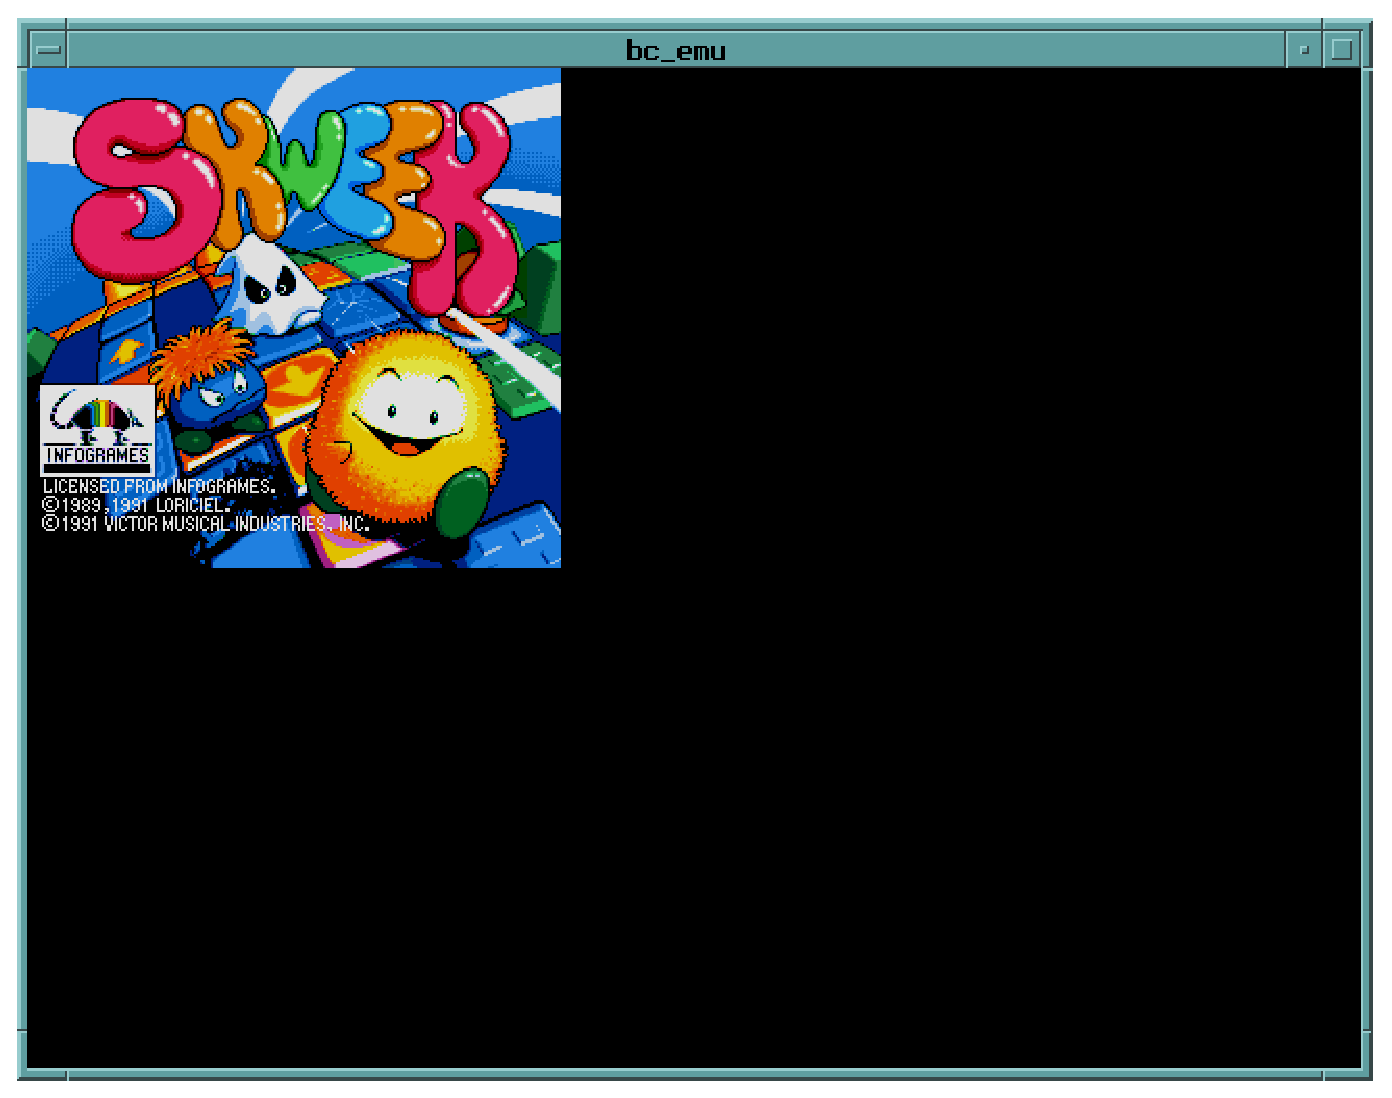
\includegraphics[width=11cm,height=8.5cm]{fig/impl_sdl}
\caption{Obrazovka programu, modul uživatelského rozhraní
	\uv{sdl}\label{fig:impl_sdl}}
\end{center}
\end{figure}

% -----------------------------------------------------------------------------
% Modul uzivatelskeho rozhrani libSDL OpenGL
% -----------------------------------------------------------------------------

\section{Modul uživatelského rozhraní libSDL s podporou
OpenGL}\label{chap:impl_sdlgl}

Modul uživatelského rozhraní libSDL s podporou OpenGL byl naimplementován pro
odlazení a ověření funkčnosti programu s více moduly. Jeho parametry i
používání jsou naprosto identické s původním modulem uživatelského rozhraní
libSDL. Jediným rozdílem je, v případě tohoto modulu, použití akcelerovaného
rozhraní OpenGL pro zobrazování obrazových dat.

Obsah struktury {\em t\_video} je použit jako textura roviny vykreslené přes
celé okno programu (640x480 pixelů) s efektem rozmazání. Snímek obrazovky
s výstupem emulace herního programu {\em Pc Genjin 2} je zobrazen na obr.
~\ref{fig:impl_sdlgl}.

\begin{figure}[ht]
\begin{center}
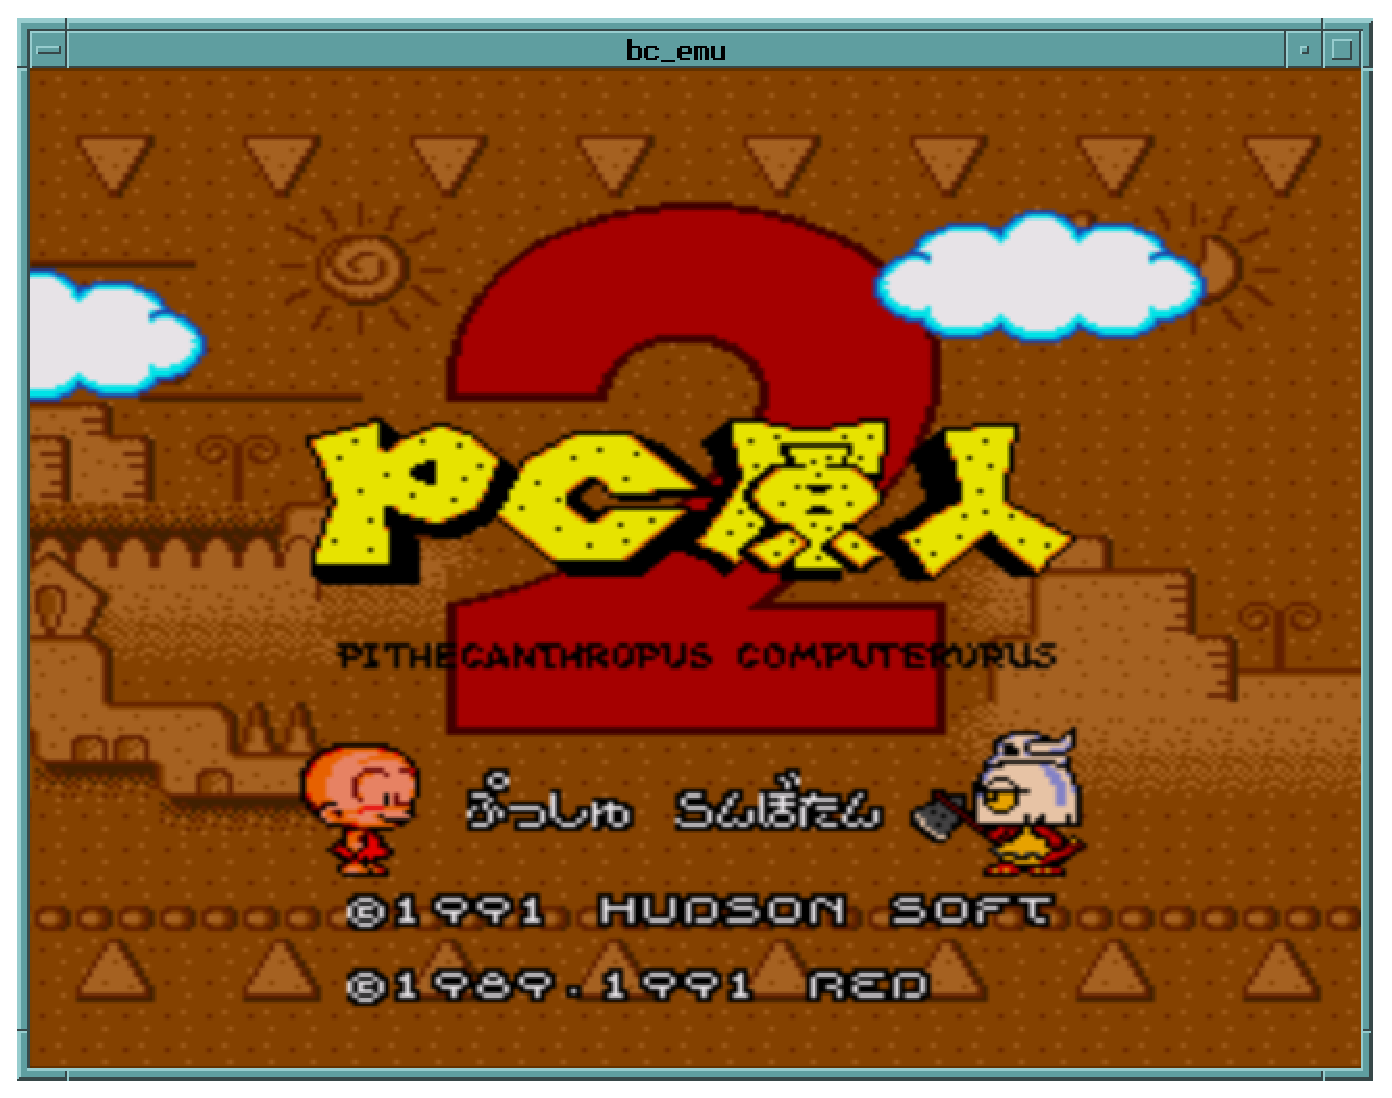
\includegraphics[width=11cm,height=8.5cm]{fig/impl_sdlgl}
\caption{Obrazovka programu, modul uživatelského rozhraní
	\uv{sdlgl}\label{fig:impl_sdlgl}}
\end{center}
\end{figure}

% -----------------------------------------------------------------------------
% Sestavovaci system CMake
% -----------------------------------------------------------------------------

\section{Sestavovací systém CMake}\label{chap:impl_cmake}

Jedním z nefunkčních požadavků na program je {\em přenositelnost kódu}, s čímž
je neodmyslitelně spojen i překlad. Tento úkol velice usnadňuje použitý
sestavovací systém CMake~\cite{wwwCMake} vyvinutý společností Kitware.

CMake slouží jako prostředník při překladu zdrojového kódu (napsaného hlavně v
jazycích C a C++). Na základě platformně nezávislého definičního souboru {\tt
CMakeLists.txt} generuje platformně závislou konfiguraci pro překlad a
sestavení programu. Program tedy může být přeložen běžně dostupnými nástroji
příslušné platformy. CMake podporuje nejběžnější platformy a kromě
definičních souborů {\tt Makefile} dokáže generovat i projektové soubory pro
nejpoužívanější vývojová prostředí Eclipse, KDevelop nebo Microsoft Visual
Studio.

Díky možnosti používání proměnných a testů v rámci zmíněného definičního
souboru {\tt CMakeLists.txt} je možné vytvořit sestavovací prostředí umožňující
jak zavedení platformních restrikcí (sestavení a připojení některého z modulů
jen na určité platformě), tak možnost personifikace sestavení začleněním pouze
určitých modulů zvolených uživatelem.

Sestavení programu je ovlivněno řadou proměnných systému CMake, z nichž většinu
nastavují testy tímto systémem prováděné. V tabulce~\ref{tab:build_opts} je pro
úplnost uveden seznam nejdůležitějších uživatelských proměnných ovlivňujících
sestavení programu včetně jejich významu.

\begin{table}[ht]
\begin{center}
\begin{tabular}{|l|l|c|}
\hline
\textbf{Proměnná} & \textbf{Význam} & \textbf{Hodnota} \\
\hline
{\tt DEBUG} & sestavení vhodné pro lazení & {\tt OFF} \\
{\tt ARCH} & cílová architektura sestavení (v současné době jen \uv{pc}) & {\tt
pc} \\
{\tt EMU\_PCE} & začlenění modulu emulátoru NEC PCEngine & {\tt ON} \\
{\tt UI\_SDL} & začlenění modulu uživ. rozhraní libSDL & {\tt ON} \\
{\tt UI\_SDLGL} & začlenění modulu uživ. rozhraní libSDL s podporou OpenGL & {\tt ON} \\
\hline
\end{tabular}
\end{center}
\caption{Uživatelské proměnné pro konfigurace sestavení pomocí
CMake\label{tab:build_opts}}
\end{table}


%%%%%%%%%%%%%%%%%%%%%%%%%%%%%%%%%%%%%%%%%%%%%%%%%%%%%%%%%%%%%%%%%%%%%%%%%%%%%%%
% bc.tex - Bachelor thesis                                                    %
% Subject: bc_emu - portable video game emulator                              %
% Chapter: Uvod                                                               %
% Author: Ondrej Balaz <ondra@blami.net>                                      %
%%%%%%%%%%%%%%%%%%%%%%%%%%%%%%%%%%%%%%%%%%%%%%%%%%%%%%%%%%%%%%%%%%%%%%%%%%%%%%%

\chapter{Testování a lazení}\label{chap:test}

Emulace videoherního systému je složitý proces sestávající z napodobování řady
funkčních součástí tohoto systému, včetně replikace jejich nedokonalostí, nebo
dokonce, chyb. Dvojnásobně toto platí o emulátorech videoherních konzolí, kdy
ve většině případů není dostupná žádná oficiální specifikace hardwaru a
neoficiální se často liší od skutečnosti, je mylná nebo vůbec neexistuje.

Od samotného počátku implementace vede k prvním viditelným výsledkům často
dlouhá cesta, na níž se nelze obejít bez důkladného odlazení a otestování
jednotlivých částí kódu, které jsou stavebními kameny výsledného programu.
Vzhledem ke způsobu práce emulátoru mohou i malé chyby snadno způsobit
řetězovou reakci ústící v neočekávané chování na místě, kde chyba vůbec
nenastala. Není třeba zmiňovat, že takové chyby se hledají nejhůře.

Tato kapitola v sekci~\ref{chap:test_debug} stručně popisuje metody jakými byl
lazen a testován vyvíjený program a v sekci~\ref{chap:test_results} shrnuje
výsledky testování současné implementace.

% -----------------------------------------------------------------------------
% Prostredky a zpusob lazeni
% -----------------------------------------------------------------------------

\section{Prostředky a způsob lazení}\label{chap:test_debug}

Interpretační způsob implementace emulátoru výrazně usnadňuje lazení programu
tím, že jsou všechny části systému představovány datovými strukturami
reprezentujícími jejich vnitřní stav (obsah interní paměti, registrů apod.) a
kód emulovaného programu je zpracováván v iteracích hlavní programové smyčky.

V průběhu vývoje je tak možné \uv{sledovat} dění uvnitř emulovaného systému
pomocí běžných ladících nástrojů umožňujících krokování a sledování obsahu
proměnných, jakým je například debugger GDB~\cite{wwwGDB}.

Kromě toho je možné využít některých ladících mechanismů implementovaných přímo
v programu. Jedním z nich je například funkce zpětného volání implementovaná
při obsluze přerušení.

Veškeré důležité informace lze v každém kroku programu vypsat pomocí ladícího
makra {\it debug()}, jehož použití je podmíněno sestavením s aktivovanou
proměnnou {\tt DEBUG} sestavovacího systému CMake. Aktivace této proměnné navíc
způsobí, že program bude na standardní chybový výstup vypisovat řadu informací
z důležitých míst v kódu (např. upozornění na provedení neošetřeného přístupu
do paměti, pokus o vykonání ilegální instrukce atd.)

K pohodlnosti lazení také přispívá modulární architektura programu, která
dovoluje jednotlivé moduly, nebo jejich části oddělit a ladit zvlášť. Tento
způsob byl využit zejména při implementaci emulace CPU HuC6280, která je z
hlediska funkčnosti nejdůležitější.

I přes všechny tyto skutečnosti může být lazení programu někdy problematické a
hodilo by se mít integrovaný ladící nástroj, který by umožňoval alespoň
sledování registrů a obsahu paměti během krokování emulovaného programu.
Implementace takového nástroje dostatečně obecného vzhledem k architektuře a
vizi dalšího rozšiřování programu o nové moduly emulátorů je rozhodně nad rámec
této práce.

% -----------------------------------------------------------------------------
% Testovani funkcnosti
% -----------------------------------------------------------------------------

\section{Testování}\label{chap:test_results}

V rané fázi vývoje probíhalo testování (hlavně implementace CPU HuC6280) pomocí
miniaturních assemblerových programů přeložených pomocí software
MagicKit~\cite{wwwMagicKit} a porovnání výsledků proti běhu stejného programu v
mírně modifikovaném emulátoru M6502~\cite{wwwM6502}.

Další testy byly provedeny sadou ROM obrazů pořízených z paměti čipových karet
HuCard speciálním zařízením PCE Pro 32M. To umožňuje záznam obrazu ROM
vloženého modulu HuCard pomocí rozhraní USB do binárního souboru.

Toto testování proběhlo na řadě odlišných obrazů ROM ve velikostech od 257~KB
do 1~MB, kdy byl porovnán průběh programu v programu {\em bc\_emu} proti
průběhu téhož programu monitorovanému ladícím nástrojem emulátoru
Mednafen~\cite{wwwMednafen}.

V průběhu testování pomocí obrazů ROM původních herních programů byla objevena
a opravena řada chyb a nesrovnalostí v emulaci CPU HuC6280. Během provádění
oprav byly na řadu citlivých míst (zápisy do paměti, vstupně-výstupní stránky
apod.) přidány ladící hlášky, které umožňují sledovat podezřelé zápisy, nebo
čtení z neexistujících adres a určit tak příčinu nefunkčnosti programu.

Stále problematickou oblastí je emulace VDC a VCE. I přes to, že byla řada chyb
opravena, je spouštění některých herních programů poznamenáno chybami v
obrazovém výstupu (artefakty, chybějící sprajty). Řada těchto chyb je
způsobena, z hlediska specifikace, nekorektním chováním programu (např. herní
program {\em Pc Genjin 2} se snaží do barevných palet zapisovat hodnoty barev
delší než $3 * 3$ bajty, což bylo třeba ošetřit použitím pouze spodních 9-ti
bajtů apod.).

I přes uvedené skutečnosti je v případě velké části obrazů ROM, které bylo
možné otestovat, emulátor plně funkční a herní programy se dají bez větších
problémů používat, např.:
{\em Doraemon Meikyu Daisakusen}, {\em Makai Prince Dorabo Chan}, {\em Pc
Genjin 2}, {\em Son Son}, {\em Xevious} nebo {\em F1 Circus}.

Za funkční jsou považovány i programy které trpí některou z
následujících kosmetických vad, vyplývajích z částečné, nebo zcela zanedbané
implementace nekritických částí specifikace. Tyto chyby lze lehce opravit v
krátkém čase:

\begin{itemize}
\item Řada herních programů (např. {\em Mesopotamia}) využívá DDA režim PSG.
	Ten není v této implementaci programu {\em bc\_emu} podporován, takže
	emulace postrádá zvukový výstup.

\item Některé herní programy (např. {\em Shinobi}) používají efekt paralaxního
	skrolování obrazu implementovaný pomocí registru {\sf BXR} pomocného
	grafického procesoru VDC. Práce s tímto registrem je naimplementována
	chybně a proto je obrazový výstup programu nesprávný.

\item Některé herní programy využívají kolizi sprajtu 0, která v současné době
	není implementována (lze pozorovat např. v pokročilejší fázi programu {\em
	Doraemon Nobita no Dorabitan Night}).

\item Řada herních programů využívá k příznaku priority sprajtu (SPBG), která v
	současné době není implementována (např. {\em Soukoban World}).

\item Některé herní programy využívají instrukci {\sc set}, jejíž implementace
	je v některých případech nefunkční.
\end{itemize}

Vzhledem k tomu, že vývoj programu proběhl za dobu uplynulých dvou semestrů a
podporovaná množina funkcí videoherního systému NEC PCEngine je oproti
existujícím emulátorům velmi malá, nemá smysl porovnávat řešení z hlediska
výkonu, nebo právě podpory jednotlivých funkcí a rozšíření systému NEC PCEngine.

%
% Platformy
%

\subsection{Platformy}

Překlad a testování programu proběhlo s výše uvedenými výsledky na všech
platformách, kde byla požadována funkčnost programu:

\begin{itemize}
\item GNU/Linux, distribuce Debian a RedHat Enterprise Linux 5 (x86-64 i i386)
\item Microsoft Windows XP SP3 (i386)
\end{itemize}

Navíc bylo ověřeno, že program je po drobných úpravách možné přeložit ve
vývojovém prostředí devkitPro~\cite{wwwDevkitPro} pro videoherní handheld
Nintendo DS. Tato platforma není podporována knihovnou SDL, takže bez
implementace specifického modulu uživatelské rozhraní nebylo možné skutečně
ověřit funkčnost.

K překladu bylo ve všech případech využito překladačů ze sady
GCC~\cite{wwwGCC}, nebo klonů na nich založených. Vzhledem k tomu, že je
program psán tak, aby byla dodržena norma ANSI C, měl by být zaručen i překlad
(vyžadující maximálně kosmetické úpravy) jinými překladači implementujícími
tuto normu.

%%%%%%%%%%%%%%%%%%%%%%%%%%%%%%%%%%%%%%%%%%%%%%%%%%%%%%%%%%%%%%%%%%%%%%%%%%%%%%%
% bc.tex - Bachelor thesis                                                    %
% Subject: bc_emu - portable video game emulator                              %
% Chapter: Zaver                                                              %
% Author: Ondrej Balaz <ondra@blami.net>                                      %
%%%%%%%%%%%%%%%%%%%%%%%%%%%%%%%%%%%%%%%%%%%%%%%%%%%%%%%%%%%%%%%%%%%%%%%%%%%%%%%

\chapter{Závěr}

Na základě dostupných informací byla nastudována architektura videoherního
systému NEC PCEngine a získané poznatky byly shrnuty do ucelené technické
specifikace uvedené v kapitole~\ref{chap:spec}. Ta posloužila jako základ pro
analýzu, návrh a následnou implementaci emulátoru tohoto systému.

S ohledem na modularitu ve smyslu možnosti rozšíření o podporu dalších
videoherních systémů, nebo uživatelských rozhraní, byl naimplementován emulátor
systému NEC PCEngine, jehož funkčnost byla úspěšně ověřena pomocí řady
původních herních programů.

Emulátor zahrnuje alespoň základní podporu všech částí základní varianty
systému NEC PCEngine a interpretačním způsobem umožňuje spouštění a provádění
herních programů uložených v souborech představujících obsah paměti ROM
původních čipových karet HuCard.

Zvolená architektura programu odděluje veškerou logiku emulace a interakce s
uživatelem do diskrétních modulů s pevně definovaným rozhraním, čímž umožňuje
nejen snadné rozšíření o podporu emulace dalších videoherních systému, ale i
zjednodušení přenositelnosti zapouzdřením kódu závislého na platformě.

Vzhledem k tomu, že program splňuje všechny zadáním specifikované požadavky a
nesrovnalosti, které se projevují při provádění emulovaných programů, jsou buď
kosmetické a lze je bez výraznějších zásahů do architektury programu odstranit,
nebo jsou způsobeny použitím nestandartních technik v rámci těchto programů a 
je třeba je řešit individuálně, lze prohlásit, že cíl této práce byl splněn.

% -----------------------------------------------------------------------------
% Dalsiho vyvoj
% -----------------------------------------------------------------------------

\section{Další vývoj}

Díky modulární architektuře umožňující implementaci podpory dalších
videoherních systémů a uživatelských rozhraní jsou možnosti rozšiřování téměř
nekonečné. Před samotným rozšiřováním tímto směrem by však mělo být zváženo
několik zásadnějších zásahů do architektury programu.

Do programu by mělo být přidáno obecné rozhraní umožňující modulům dotazovat se
na hodnoty konfiguračních klíčů (např. moduly uživatelského rozhraní by měly
mít možnost konfigurce vstupních zařízení, rozlišení obrazovky, formátu zvuku
apod.).

Dalším možným rozšířením je implementace nového typu modulu - ladícího
nástroje pro emulovaný program, který by uměl na obecné úrovni (samozřejmě by
autor modulu emulátoru musel provést nastavení) sledovat registry a paměťové
oblasti emulovaného systému, případně krokovat program.

Implementace ladícího nástroje by jistě pomohla při dalším zdokonalování modulu
emulátoru systému NEC PCEngine. Kromě odstranění drobných chyb a doimplementace
chybějících, v kapitole~\ref{chap:test_results} zmíněných, nekritických částí
specifikace, by bylo vhodné zdokonalit kód PSG a přidat podporu pro některá
populární rozšíření.

Po zásadnějších úpravách a stabilizaci architektury může být zajímavou výzvou
přenést program {\em bc\_emu} na videoherní handheld Nintendo DS. S drobnými
úpravami je už nyní možné pro tento systém přeložit jádro programu. Dalším
krokem je nastudování programového rozhraní knihoven devkitPro a implementace
modulu uživatelského rozhraní. Vzhledem k výkonu procesoru tohoto systému mohou
nastat potíže s výkonem. Dalším směrem vývoje proto může být optimalizace
emulačního kódu při zachování přenositelnosti.


% -----------------------------------------------------------------------------
% Main document / bibliography
% -----------------------------------------------------------------------------

\bibliographystyle{plain}
{
	\def\CS{$\cal C\kern-0.1667em\lower.5ex\hbox{$\cal S$}\kern-0.075em $}
	\bibliography{bt_balazond}
}

% -----------------------------------------------------------------------------
% Main document / appendices
% -----------------------------------------------------------------------------

\appendix

%*****************************************************************************
\chapter{Seznam použitých zkratek}

\begin{description}
\item[ANSI] American National Standards Institute
\item[BAT] Background Attribute Table
\item[CPU] Central Processing Unit
\item[DDA] Direct Data Access
\item[DMA] Direct Memory Access
\item[I/O] Input/Output
\item[IRQ] Interrupt Request
\item[LFO] Low Frequency Oscillator
\item[NEC] Nippon Electronic
\item[NMI] Non-Maskable Interrupt
\item[NTSC] National Television System Committee
\item[PAL] Phase Alternating Line
\item[PSG] Programmable Sound Generator
\item[RAM] Random Access Memory
\item[RF] Radio Frequency
\item[ROM] Read Only Memory
\item[SAT] Sprite Attribute Table
\item[VCE] Video Color Encoder
\item[VDC] Video Display Controller
\item[VRAM] Video Random Access Memory
\item[WDC] Western Digital Company
\end{description}

%*****************************************************************************
\chapter{Uživatelská příručka}

Text tohoto dodatku popisuje způsob sestavení, spuštění a ovládání programu
{\em bc\_emu}.

\section{Sestavení programu}

Sestavení programu není nutné provádět na platformách GNU/Linux (i386 a x86-64
s aktuální verzí knihovny glibc) a Microsoft Windows. Pro tyto platformy jsou v
příslušných adresářích na přiloženém disku DVD (viz. dodatek~\ref{apdx:dvd})
připraveny binární soubory, které stačí spustit.

Pro sestavení je nutné mít v systému nainstalovány následující prerekvizity:
{\em CMake 2.8}, {\em překladač jazyka C (gcc, mingw-gcc)}, {\em
libSDL1.2-devel}, {\em make}. Samotný postup sestavení je následující:

\begin{enumerate}
\item zkopírování adresáře {\tt src} z přiloženého DVD na pevný disk
\item vytvoření adresáře sestavení {\tt build}
\item konfigurace sestavení souborem {\tt src/CMakeLists.txt} do adresáře {\tt
	build} pomocí sestavovacího systému  CMake (viz.~\cite{wwwCMake})
\item spuštění programu make v adresáři {\tt build}
\end{enumerate}

\section{Spuštění programu}

Program {\em bc\_emu} se spouští pomocí příkazové řádky s přepínači v krátké
UNIXové notaci (např. {\tt -h}). Pro úspěšné spuštění emulace musí být
programu kromě jména obrazu ROM předána ještě informace o tom jaký modul
emulátoru ({\tt -e}) a uživatelského rozhraní ({\tt -u}) má být použit.

Pro demonstraci veškerých schopností programu {\em bc\_emu} stačí program
spustit jedním z této dvojice příkazů:

\noindent
{\tt bc\_emu -e pce -u sdl obraz\_rom.pce}

\noindent
{\tt bc\_emu -e pce -u sdlgl obraz\_rom.pce}

První spustí emulaci se zobrazováním výstupního obrazu pomocí knihovny libSDL,
druhý pomocí knihovny OpenGL.

V případě použití dodaného binárního souboru, zkompilovaného překladačem MinGW
GCC pro Microsoft Windows, jsou standardní i chybový výstup přesměrovány do
souborů {\tt stderr.txt} a {\tt stdout.txt} vytvořených v cestě odkud byl
program spuštěn. Proto i ladící verze programu nevypisuje žádné hlášky do
konzolového okna.

\section{Ovládání programu}

V rámci obou modulů uživatelského rozhraní ({\em sdl} i {\em sdlgl}) lze použít
k ovládání programu klávesy uvedené v tabulce~\ref{tab:manual_keys} (tabulka je
shodná s tabulkou~\ref{tab:sdl_keymap} a je opakovaně uvedena pro větší
přehlednost této příručky).

\begin{table}[ht]
\begin{center}
\begin{tabular}{|l|l|}
\hline
\textbf{Klávesa} & \textbf{Význam} \\
\hline
{\tt <nahoru>} & směrový kříž herního ovladače, směr nahoru \\
{\tt <dolů>} & směrový kříž herního ovladače, směr dolů \\
{\tt <vlevo>} & směrový kříž herního ovladače, směr vlevo \\
{\tt <vpravo>} & směrový kříž herního ovladače, směr vpravo \\
{\tt <enter>} & tlačítko \uv{Start} herního ovladače \\
{\tt a} & tlačítko \uv{I.} herního ovladače \\
{\tt s} & tlačítko \uv{II.} herního ovladače \\
\hline
{\tt r} & restart emulace \\
{\tt q} & ukončení programu \\
\hline
\end{tabular}
\end{center}
\caption{Mapování kláves\label{tab:manual_keys}}
\end{table}


%*****************************************************************************
\chapter{Obsah přiloženého DVD}\label{apdx:dvd}

\noindent
Na přiloženém DVD jsou umístěny následující adresáře: \\

\noindent
\begin{tabular}{ll}
{\tt bin\_linux\_i386} &    binární soubory pro GNU/Linux (i386) \\
{\tt bin\_linux\_x86-64} &  binární soubory pro GNU/Linux (x86-64) \\
{\tt bin\_win32} &          binární soubory pro Microsoft Windows (32bit) \\
{\tt rom\_com} &            obrazy ROM (komerční) \\
{\tt rom\_free} &           obrazy ROM (volně dostupné) \\
{\tt src} &                 zdrojový kód programu {\em bc\_emu} \\
{\tt src\_doc} &            dokumentace ke zdrojovému kódu (HTML) \\
{\tt thesis} &              soubory PDF s tímto textem (tisk, online) \\
{\tt thesis\_src} &         zdrojový kód tohoto textu pro systém \LaTeX \\
\end{tabular}

% -----------------------------------------------------------------------------
% Main document / end
% -----------------------------------------------------------------------------

\end{document}
